\chapter{Proving Compatibility of Consistency Relations
    \pgsize{40 p.}
}
\label{chap:compatibility}

%\todo{Check whether we can better derive necessity of compatibility in terms of transformations to being able to find consistent models at all. Does only ensure that transformations can at least, if properly defined, find consistent models.}
\todo{Final müssen wir diskutieren, wie sich Inkompatibilitäten darauf auswirken, ob eine Ausführungsstrategie einen konsistenten Zustand findet. Im Optimalfall zeigen wir, dass Kompatibilität das Orchestrierungsproblem vereinfacht!}

\mnote{Artifacts and correctness in modular consistency specification}
We have defined in \autoref{chap:correctness} that transformations are composed of \glspl{consistency relation} and \glspl{consistency preservation rule} that preserve them.
We especially focus on binary relations and according preservation rules, which concern two metamodels.
Multiple transformations can be combined to a network with an orchestration and application function that executes the transformation in a determined order to restore consistency after changes to concrete models.
We have also identified correctness notions and came to the conclusion that with modular, binary transformations combined to a network the individual consistency preservation rules must be correct with respect to the consistency relations they preserve and the orchestration and application functions must be correct with respect the combination of all consistency relations, such that all models are consistent to all consistency relations after executing the transformations.

\mnote{Consistency relations are correct by construction}
As a consequence of the identified correctness notion, we also found that the underlying consistency relations themselves can, from a theoretical perspective, be considered correct by construction, as there is no other artifact (be it explicit or only implicitly given) with respect to which it has to be correct.
Since we assume transformations to be developed independently and reused in a modular way, we can especially not assume a monolithic consistency relation to which the modular consistency relations must be correct (cf.\ \autoref{chap:correctness:notions:dimensions}).
We have, however, already given examples for cases in which binary consistency relations are somehow contradictory.
This is the case if the developers of the individual transformations have different, conflicting notions of consistency between the metamodels.
In the worst case, this can lead to the situation that no single set of models would be considered consistent to a set of binary consistency relations, which is obviously unwanted behavior.
We have discussed an abstract example for that case already in \autoref{chap:correctness:notions:relations}.

\begin{figure}
    \centering
    %% From motivational_example in MPM4CPS paper

\newcommand{\hdistance}{14em}
\newcommand{\classwidth}{6em}

\begin{tikzpicture}

% Person
\umlclassvarwidth{person}{}{Person\sameheight}{
firstname\\
lastname\\
address\\
income
}{\classwidth}

% Employee
\umlclassvarwidth[,above right=2em and \hdistance of person.east, anchor=south]{employee}{}{Employee\sameheight}{
name\\
socsecnumber\\
salary
}{\classwidth}

\umlclassvarwidth[,below=4em of employee.south, anchor=north]{resident}{}{Resident\sameheight}{
name\\
address\\
socsecnumber
}{\classwidth}


% CONSISTENCY RELATIONS
\draw[consistency relation] (person.north) |- node[pos=0, above left] {$p$} node[pos=0.75, above] {$\consistencyrelation{CR}{PE}$} node[pos=1, above left] {$e$} (employee.west);
\draw[consistency relation] (employee.south) -- node[pos=0, below left] {$e$} node[right, align=left] {$\consistencyrelation{CR}{ER}$ / $ \consistencyrelation{CR}{ER}'$}% /\\ $R'_{ER}$} 
node[pos=1, above left] {$r$} (resident.north);
\draw[consistency relation] (resident.west) -| node[pos=0, below left] {$r$} node[pos=0.25, below] {$\consistencyrelation{CR}{PR}$ / $\consistencyrelation{CR}{PR}'$} node[pos=1, below left] {$p$} (person.south);

\node[consistency related element, below left=5em and 2em of person.south west, anchor=north west] {
$\begin{aligned}
    \consistencyrelation{CR}{PE} =\; &
        \setted{\tupled{p,e} \mid %\\
        %& 
        \mathvariable{p.firstname} + "\text{\textvisiblespace}" + \mathvariable{p.lastname} = \mathvariable{e.name}%\\
        %& 
        \land \mathvariable{p.income} = \mathvariable{e.salary}
    }\\[0.3em]
    \consistencyrelation{CR}{PR} =\; &
        \setted{\tupled{p,r} \mid %\\
        %& 
        \mathvariable{p.firstname} + "\text{\textvisiblespace}" + \mathvariable{p.lastname} = \mathvariable{r.name}%\\
        %& 
        \land \mathvariable{p.address} = \mathvariable{r.address}
    }\\
    \consistencyrelation{CR}{PR}' =\; &
        \setted{\tupled{p,r} \mid %\\
        %& 
        \mathvariable{p.lastname} + ",\text{\textvisiblespace}" + \mathvariable{p.firstname} = \mathvariable{r.name}%\\
        %& 
        \land \mathvariable{p.address} = \mathvariable{r.address}
    }\\[0.3em]
    \consistencyrelation{CR}{ER} =\; &
        \setted{\tupled{e,r} \mid %\\
        %& 
        \mathvariable{e.name} = \mathvariable{r.name} %\\
        %& 
        \land \mathvariable{e.socsecnumber} = \mathvariable{r.socsecnumber}
    }\\
    \consistencyrelation{CR}{ER}' =\; &
        \setted{\tupled{e,r} \mid %\\
        %& 
        \mathvariable{e.name.toLower} = \mathvariable{r.name} %\\
        %& 
        \land \mathvariable{e.socsecnumber} = \mathvariable{r.socsecnumber}
    }
\end{aligned}$
};

\end{tikzpicture}
    \caption[Three metamodels with (in)compatible consistency relations]{Derivation of \autoref{fig:networks:three_persons_example}: Three simple metamodels for persons, employees and residents, and three binary relations $R_{PE}, R_{PR}, R_{ER}$ between each pair of them, with $R'_{PR}$ as an alternative for $R_{PR}$ and $R'_{ER}$ as an alternative for $R_{ER}$.}
    \label{fig:compatibility:three_persons_example_extended}
\end{figure}

\mnote{Intuitive compatibility in the running example}
We recapture the running example defined in \autoref{fig:networks:three_persons_example} and extend it with alternatives for two of the binary consistency relations in \autoref{fig:compatibility:three_persons_example_extended}.
The example contains three pairwise consistency relations between persons, employees and residents and are defined in a way such that none of them can be omitted, because each pair shares a unique overlap in their attributes.
In that example, the consistency relations $R_{PE}, R_{PR}$ and $R_{ER}$ are fulfilled if for any person (and analogously employee and resident) in the models there is exactly one employee and one resident, which fulfill the relations for names and further attributes defined by the consistency relations.
As we will see later, it is of special importance that there is always only one such corresponding element, e.g., that there are not two employees fulfilling the relation to a single resident.
Intuitively, these consistency relations are \emph{compatible}, as they lead to a reasonable set of models that are considered consistent to each other.

\begin{figure}
    \centering
    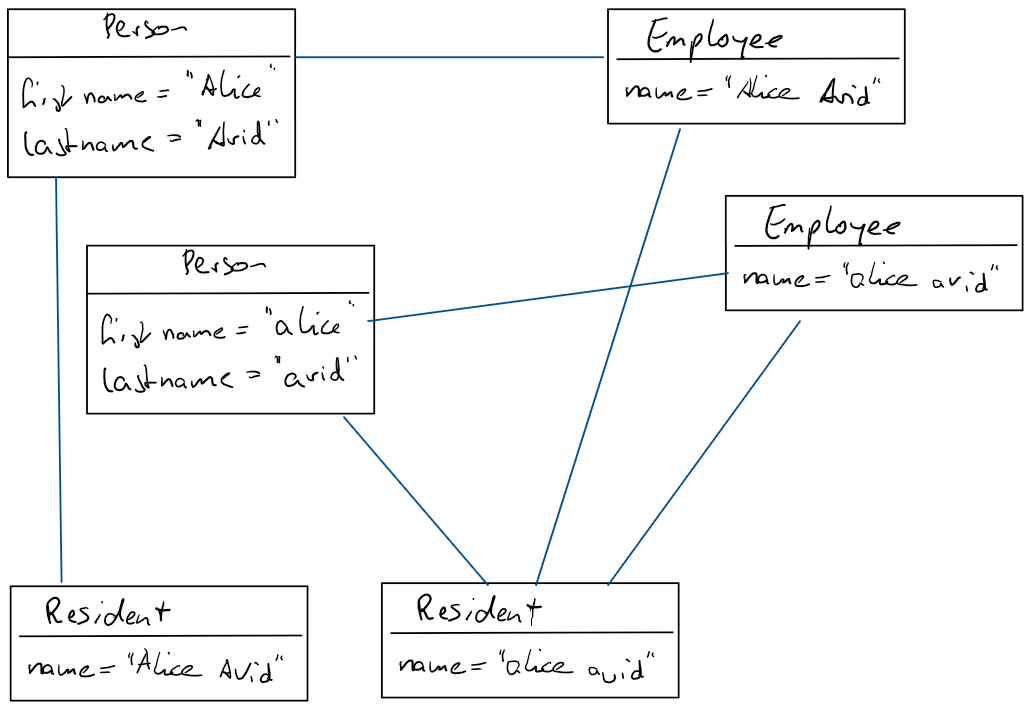
\includegraphics[width=\textwidth]{figures/correctness/compatibility/intuitive_incompatibility.png}
    \caption[Example for an intuitive notion of incompatibility]{Elements required by the consistency relations in \autoref{fig:compatibility:three_persons_example_extended} for a resident with the name \enquote{Alice Avid}.}
    \label{fig:compatibility:intuitive_incompatibility}
\end{figure}

\mnote{Intuitive incompatibility in the modified running example}
In contrast, considering consistency relation $R'_{PR}$ instead of $R_{PR}$, the relations can never be fulfilled, because the concatenation of $firstname$ and $lastname$ from person to employee and from person to resident is conflicting.
The relation between employees and residents assumes to be $firstname$ and $lastname$ to be concatenated in the same order, whereas the relations to person do not.
Fulfilling these relations would require an infinitely large model, as each cycle through the relations swaps $firstname$ and $lastname$ and appends an additional comma due to the relation between person and resident.
Thus, the set of consistent model tuples would be empty.

\todo{Maybe leave the following out, or move it to the more fine-grained part}
\mnote{More detailed incompatibility in the modified running example}
In addition, considering consistency relation $R'_{ER}$ instead of $R_{ER}$, no models containing residents with a name not written in lower case can be consistent to all relations, as depicted in \autoref{fig:compatibility:intuitive_incompatibility}, which, for reasons of simplicity, omits all other attributes than the names.
A resident with a non-lower-case name requires a person with equally written first and last name to exist.
This, in consequence requires an employee with an equally written name to exist.
The relation $R'_{ER}$ now requires a resident with the name written in lower case to exist, which again requires a person with the lower-case name and this, in turn, requires an employee with the lower-case name.
In consequence, however, the resident with the lower-case name would correspond to both the employee with the original and the lower-case name, whereas the resident with the original name does not correspond to any employee.
More intuitively speaking, it is impossible to find an employee that fulfills the consistency relation $R'_{ER}$ for a resident with a non-lower-case name.
This is what we will call and later precisely define as an \emph{incompatibility} of the consistency relations, as they define constraints that cannot be fulfilled at the same time.
This can always occur if there is a cycle in the graph induced by the combined consistency relations.

\mnote{Incompatibilites prevent transformations from finding consistent models}
On the one hand, such incompatibilities are unwanted, as they indicate that developers have different, contradictory notions of consistency.
On the other hand, the contradictions can easily lead to the situation that the transformations are not able to find consistent models or at least that their orchestration for finding consistency models becomes unnecessarily difficult.
Therefore, in this chapter we first discuss some scenarios to identify an intuitive notion of compatibility, which we then use to define a precise notion of \emph{compatibility}.
Afterwards, we develop a formal, inductive approach to prove compatibility of relations, which we base on a formal framework for which we prove correctness and then derive a practical approach for the transformation language \gls{QVTR} that uses that formal framework.
The approach is based on the insight that consistency relations having a specific kind of tree structure are compatible and that removing a specific kind of redundant relations is compatibility-preserving.
This chapter thus constitutes our contribution \contributionref{contrib:correctness:compatibility} and answers the following research question:

\researchquestionrepeat{rq:correctness:compatibility}

% In this article, we consider the relations defined by bidirectional transformations.
% We clarify the notion of \emph{compatibility} of these relations and develop an approach to prove compatibility of relations in a given network of transformations.
% To achieve this, we formally define a notion of consistency, based on fine-grained consistency relations, as well as compatibility.
% Building on this formalism, we are able to derive an inductive, formal approach for proving compatibility of relations by identifying those that are redundant.
% The essential idea is that if consistency relations have a specific kind of tree structure, we are able to show that they are inherently compatible.
% Furthermore, we show that adding redundant relations to such a tree preserves compatibility.
% In consequence, reducing an arbitrary network of relations to a tree by removing redundant relations proves compatibility.
% Finally, we present an operationalized approach based on that formal approach for \qvtr to prove compatibility of a network of \qvtr relations.
% That approach transforms \qvtr relations into first-oder logical formulae and finds redundant relations by applying an SMT solver.
% % We propose an approach that is able to prove that transformations are compatible, on the example of QVT-R. The approach represents the transformation rules as a graph of metamodel elements with consistency relations between them. Its goal is to find an equivalent set of trees of consistency relations, which are compatible due to the inherent absence of cycles. To achieve that, it decomposes the graph into independent subsets and then removes redundant consistency relations within existing cycles. To prove redundancy of a relation, cycles of relations are transformed into logical expressions and evaluated with an SMT solver. 
% More detailed, we make the following contributions:
% \begin{description}[leftmargin=\parindent]
%     \item[\contributionlabel{contrib:formalization}{Compatibility Formalization}{C1}:] We formalize a notion of consistency and precisely define \emph{compatibility} of relations in a network of transformation.
%     \item[\contributionlabel{contrib:formalapproach}{Formal Approach}{C2}:] We define a formal, inductive approach for proving compatibility of relations based on a notion of redundancy and relation trees. % and proving that such trees are compatible and that redundancy preserves compatibility.
%     \item[\contributionlabel{contrib:operationalizedapproach}{Operationalized Approach}{C3}:] We propose an approach that applies the formalism to %transformation languages. %and thus enables proving compatibility of transformations defined in a transformation language. 
%     %We especially discuss the approach application to 
%     \qvtr and show how a translation to logical formulae and the usage of SMT solver can be used to prove compatibility.
%     \item[\contributionlabel{contrib:evaluation}{Applicability Evaluation}{C4}:] While correctness of the approach is given by construction and proven on the formalism, we apply the approach to case studies to show applicability of the approach. 
% \end{description}

\mnote{Compatibility can be proven, incompatibility can not}
We will see that it is in general not possible to prove that transformation are incompatible if the language, in which the relations are described, is undecidable, such as \gls{QVTR}.
We can, however, at least conservatively prove that transformation are compatible.
Thus, if our approach proves compatibility, the transformation are actually compatible, but not vice versa.
This enables transformations developers to check their transformations for compatibility both on-the-fly during transformation development, if developed for a specific scenario, or a posteriori during their combination, according to the scenarios introduced in \autoref{chap:networks:specification_process}.
Especially in the first scenario, developers can immediately react to the introduction of incompatibilities during transformation development.



%%%
%%% COMPATIBILITY NOTION
%%%
\section{Towards a Notion of Compatibility}

\mnote{Modular relations induce monolithic ones}
A set of binary consistency relations induces a monolithic, $n$-ary relation, also called \emph{global relation}, as discussed in \autoref{chap:correctness:notions:relations}.
A monolithic relation $\consistencyrelation{R}{}$ for metamodels $\metamodelsequence{M}{n}$ and pairwise consistency relations $\consistencyrelation{R}{i,j}$ is defined by:
\begin{align*}
    \consistencyrelation{R}{} = \setted{\tupled{\model{m}{1}, \dots, \model{m}{n}} \mid \bigwedge\limits_{1 \le i < j \le n} \tupled{\model{m}{i}, \model{m}{j}} \in \consistencyrelation{R}{i,j}}
\end{align*}
As discussed before, the consistency relations are correct by definition and so is the induced global relation, even if it is empty.
It is, however, unclear whether the relations are \enquote{reasonable} in combination.
%However, just because the induced monolithic relation does, for example, only contain one consistent tuple of models, this may not imply that it is not as intended.

\begin{figure}
    \centering
    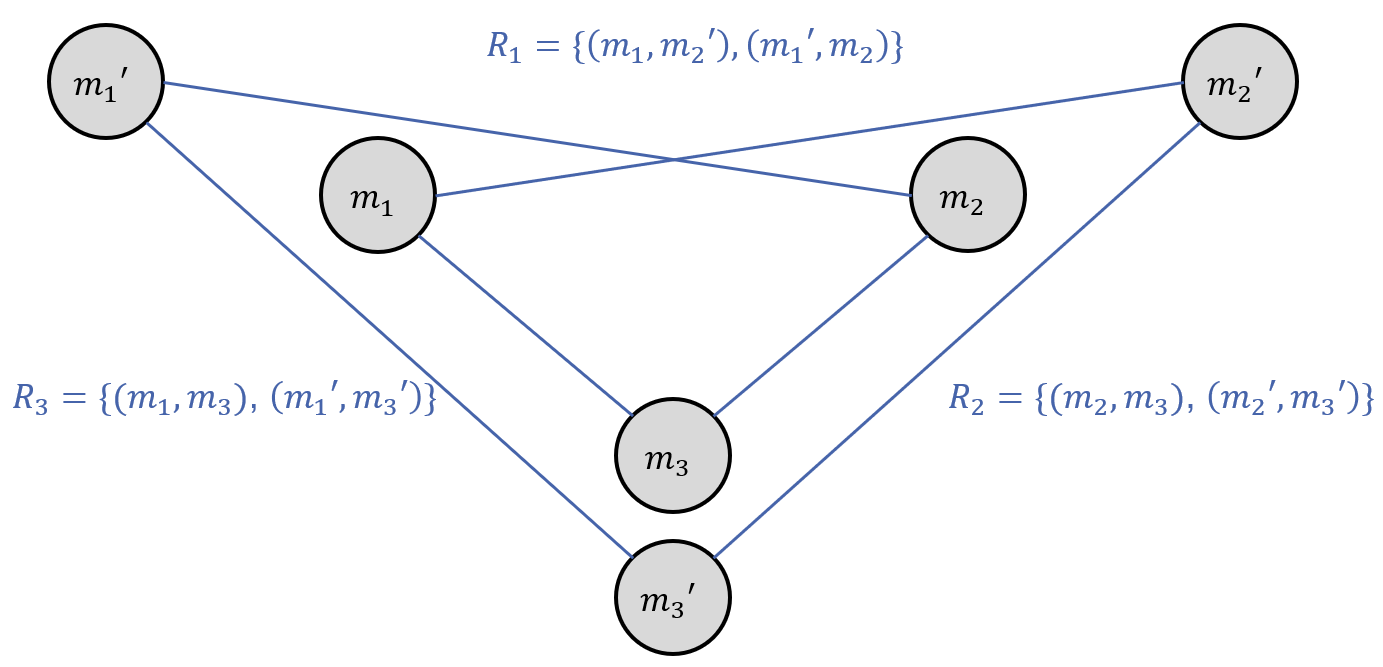
\includegraphics[width=\textwidth]{figures/correctness/compatibility/empty_global_relation.png}
    \caption[Consistency relations that imply an empty global relation]{Example for consistency relations that imply an empty global relation}
    \label{fig:compatibility:empty_global_relation}
\end{figure}

\mnote{Empty induced global relations indicate incompatibility}
In fact, if the relations induce an empty global relation, these relations do actually not properly fit to each other, because no single tuple of models would be considered consistent, thus no system could be consistently described.
We would thus consider such relations incompatible.
\autoref{fig:compatibility:empty_global_relation} shows an extended version of the example already given in \autoref{chap:correctness:notions:relations}, inducing an empty global relation.
This is an abstraction of the concrete examples, which we have already discussed for our our running example, in which modified consistency relations lead to an empty set of consistent model tuples, due to conflicting conversions and concatenations of names between persons, residents and employees.

\mnote{Goal of identifying incompatible relations}
There may, however, be more cases than empty induced global relations that we want to exclude by considering the relations incompatible.
In general, the goal of finding incompatibilities and excluding them is twofold:
First, we may want to identify that different developers of modular relations have an incompatible notion of consistent, such that the results would never be as expected.
This is what we have seen in the examples with the name relations.
We want to exclude these cases, because developers will not want to combine transformation based on relations that are contradicting.
Second, incompatibilities may lead to transformations not being able to find consistent models, so the orchestration would not be able to execute transformations in an order that achieves a consistent state.
If we, for example, encoded the relations from the running with the inverse concatenation of $firstname$ and $lastname$ ($R'_{PR}$) into transformations, each cycle in which the transformation are executed would produce one new person, employee, and resident, with swapped $firstname$ and $lastname$ and a comma appended to $lastname$.
In consequence, transformations would not be able to find a consistent state and, if not stopped preemptively, be executed endlessly.
Thus we also want to exclude such cases, because it can prevent a transformation network from termination.

%\begin{itemize}
    %\item We discussed that we are not interested in correctness of modular relations w.r.t. one monolithic relations, as that relations is usually unknown and thus correctness cannot be checked (cf ~\autoref{chap:correctness:notions:dimensions})
    %\item This would mean that modular relations are correct by construction
    %\item Although relations are, theoretically, correct by construction, we have seen that there are relations, for which we may say that they do not properly work together, i.e., they are \emph{incompatible}, as discussed in \autoref{chap:correctness:notions:relations}
    %\item There, we had three binary relations, which, taken together, do not impose an overall relation containing any consistent set of models, see \autoref{fig:compatibility:empty_global_relation}
    %\item We have already given a more concrete example for that case from our running example before.
    %\item It is obvious that we may not want to have an induced global relation that is empty, however, there may be more cases that we want to exclude.
    %%\item Exclude somehow defined \emph{incompatibilites} may be wanted for two reasons: First, we may want to identify that different developers of modular relations have an incompatible notion of consistency, such that the result would never be as expected (this is what we have seen for the names). Second, incompatibilites may lead to transformations not being able to find a consistent solution, so the orchestration would not be able to execute transformations to achieve a consistent state. To show that, we extend the relations example to a transformation example, showing that no consistent state can be reached, i.e., for an added person no consistent employees etc. can be found
%\end{itemize}


%%
%% OBSOLETE RELATIONS
%%
\subsection{Necessity of Obsolete Relation Elements}

First option: Remove "obsolete" relation elements
\begin{figure}
    \centering
    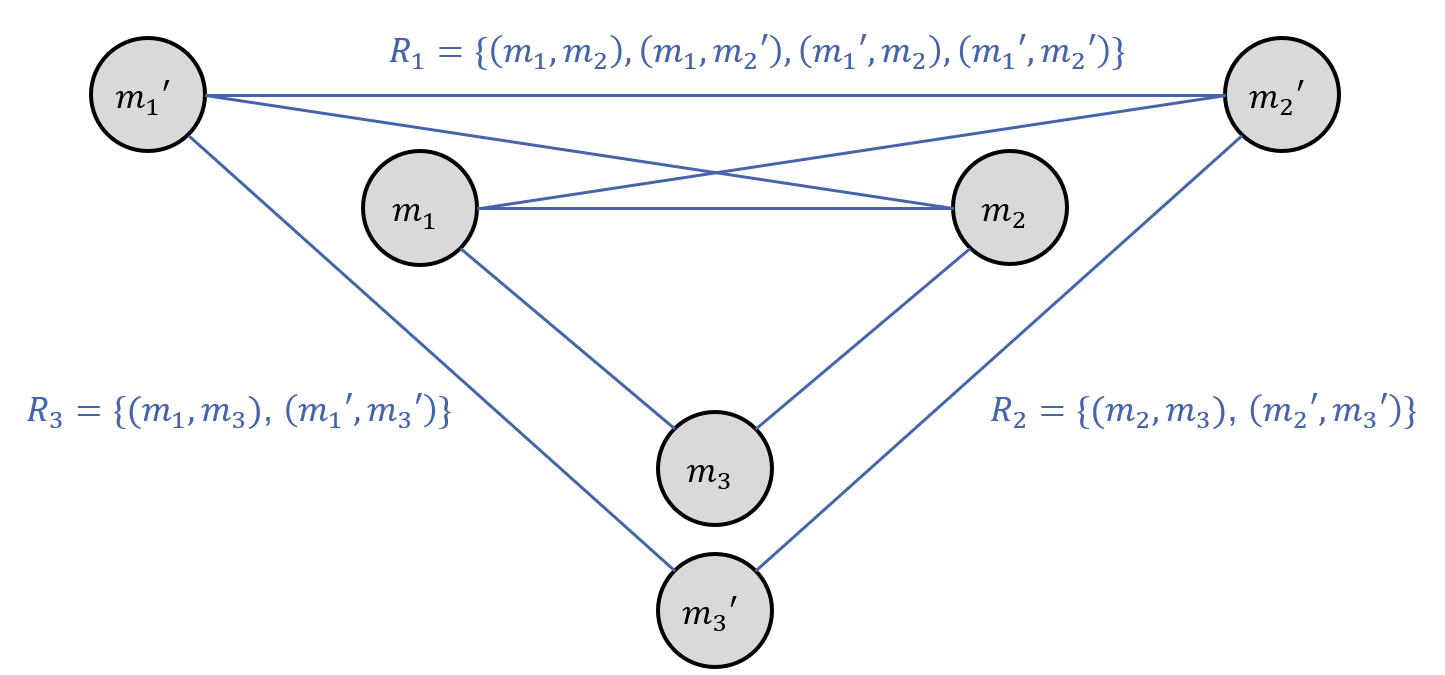
\includegraphics[width=\textwidth]{figures/correctness/compatibility/obsolete_relations.png}
    \caption[Example for obsolete elements in consistency relations]{Example for \enquote{obsolete} models pairs in consistency relation $R_1$, which can never occur in a globally consistent set of models}
    \label{fig:compatibility:obsolete_relations}
\end{figure}
\begin{itemize}
    \item A first option might be to say that there should not be model pairs in the relations for which no globally consistent set of models can be found (give an abstract example for that)
    \item However, in consequence a transformation could not produce such models, which might be necessary as transient (intermediate) states: E.g. a UML and Java code model are consistent when the same classes and interface with the same (in Java potentially empty) methods are present. In fact, a UML model is consistent with all (usually infinite) Java models with the same classes and methods, but with arbitrary method implementation. PCM and UML are consistent when components are realized as classes implementing the provided interfaces and thus their methods. Analogously, each component is represented by a Java class implementing the provided interfaces, but having an implementation that has some default functionality (be it logging or something more component-specific). Forbidding relations elements that can never be globally consistent would forbid that the relation between UML and Java allows Java models with empty method implementations for UML classes representing components. This would, however, require the relation/transformation between UML and Java know about components, which should not be the case due to modularity and independent development. Additionally, even in the concrete setup in which PCM is used, if a method is added to an interface of a class in UML which is a provided interface of its component in UML, the transformations may first create the Java method with an empty body, then propagate the method to the PCM interface and then propagate the default implementation of that method from PCM to Java. In this case, the transient state with the empty method body in Java is passed. Forbidding that would require an appropriate orchestration, i.e., first propagating the information across PCM, which could be defined for this specific case but not automatically decided in general, or the UML-Java transformation would have to consider that the Java implementation may not be empty, which, as discussed, contradicts modularity.
    \item In general, this case is reflected in \autoref{fig:compatibility:obsolete_relations}, which shows two pairs in $R_1$, which can never occur in a globally consistent model, because the implied global relation is .... and does not contain those model pairs
\end{itemize}


%%
%% UNWANTED BEHAVIOR
%%
\subsection{Prevention from Finding Proper Solutions}

Second attempt: Derive incompatibility notion from unwanted behavior
\begin{figure}
    \centering
    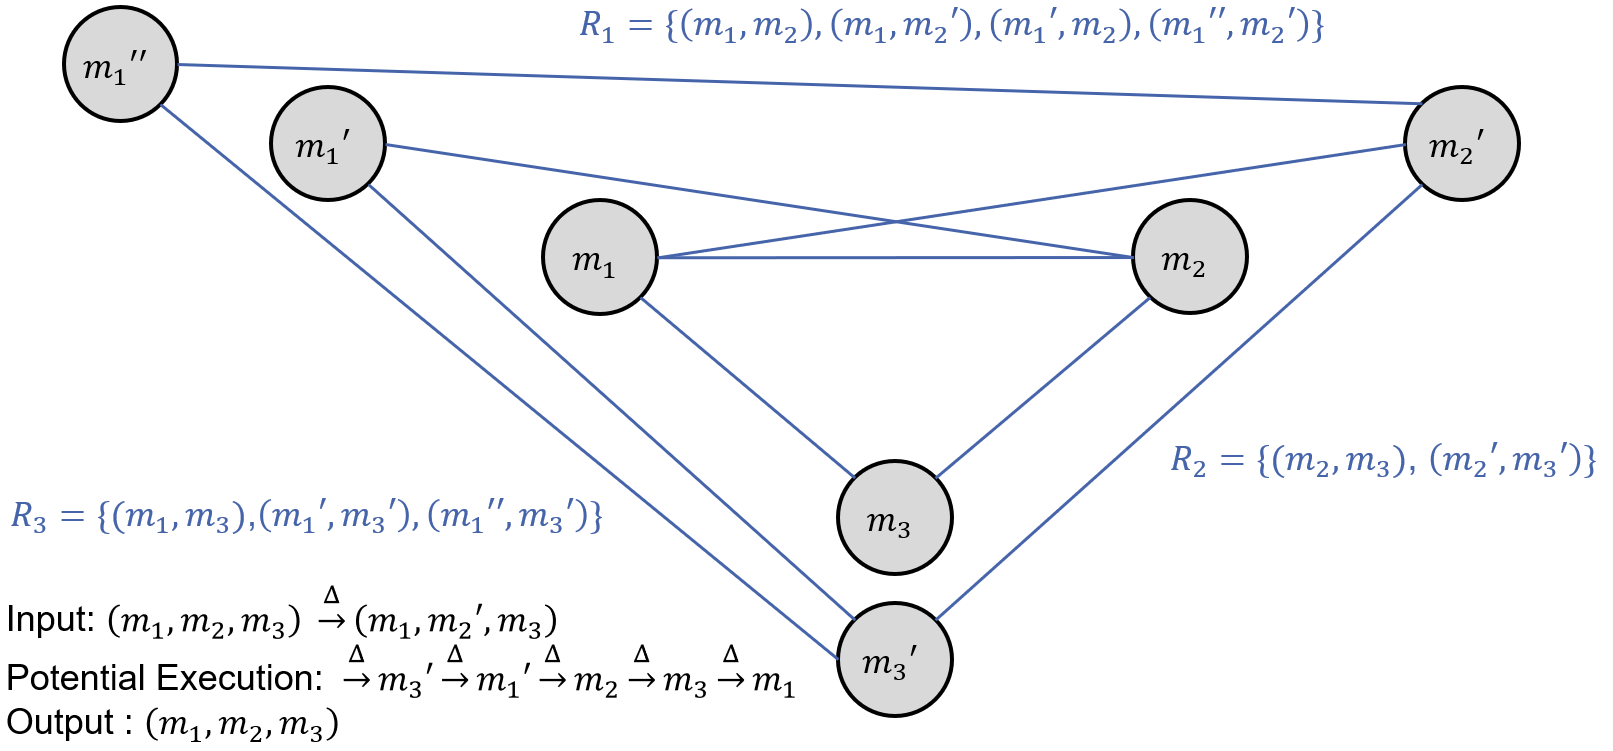
\includegraphics[width=\textwidth]{figures/correctness/compatibility/unwanted_behavior.png}
    \caption[Example for the unwanted rejection of a user change]{Example for the rejection of a user change because of consistency relations containing model pairs that are never globally consistent}
    \label{fig:compatibility:unwanted_behavior}
\end{figure}
\begin{itemize}
    \item Considering the example in \autoref{fig:compatibility:unwanted_behavior}, we start with $A_1, B_1, C_1$ and have a user change of $B_1$ to $B_2$. Apart from the input models, only $A_3, B_2, C_2$ are globally consistent. So we would expect the transformations to find the latter models. Because of also having consistency relations to $A_2$ and transformation that locally select $A_2$ (because they do not know that there is no globally consistent state with $A_2$), passing across that model can lead to resulting in $A_1, B_1, C_1$ again. We did not define that requirement yet because it is not essentially necessary, but usually user may not want their changes be undone by a transformation, at least if there was another set of consistent models reflecting their change.
    \item Thus, we would call this behavior unwanted.
    \item Note that this scenario is different from the described scenario with empty Java method bodies, because in that case there are models for which an empty Java method body occurs in a globally consistent states (those in which the method does not realize a method of a provided interface of a component). Thus if the corresponding class does not realize a component but an ordinary class, it would be fine that it is consistent to the UML class with an empty body. In contrast, in the case described here, there is no single set of models in which $A_2$ was consistent.
\end{itemize}


%%
%% COMPATIBILITY NOTION
%%
\subsection{An Information Notion of Compatibility}

Derived (informal) notion of compatibility:
\begin{itemize}
    \item Models are problematic if
    \begin{itemize}
        \item They can be locally consistent (according to one relation) to another model
        \item They are never globally consistent (not contained in any set of models that is consistent)
    \end{itemize}
    \item $A_2$ was such a model only being locally consistent with $B_1$ and $C_2$, but those are inconsistent.
    \item Case Analysis:
    \begin{itemize}
        \item $A_2$ is created by a user: Adapting this model is unwanted, as the user introduced it
        \item $A_2$ is created by a transformation: Either created because $B_1$ or $C_2$ was introduced. However, there are other $A_X$ to which $B_1$ and $C_2$ are consistent (otherwise they would be in the same situation as $A_2$), so the transformations should better select such a different $A_X$, as $A_2$ will never be consistent
    \end{itemize}
    \item As we can see from the example, considering such models does not provide any benefits (because they do never occur in a globally consistent state), but they can easily prevent transformations from finding a consistent state.
    \item We can derive the following informal notion of incompatibility: For each model in a relation, a globally consistent model tuple must exist
    \item More precisely, we will define this notion at the level of model elements rather than complete models, as transformations are usually defined in terms of rules that affect only some of the elements of models, such as a limited set of meta-classes and their properties.
\end{itemize}

\todo{In general, an empty set of consistent models can be intended. Without knowing about "semantics" it is impossible to validate whether restrictions are intended or not. However, we want to identify unintended situations, so we may define situations that we actually do not want to support, because there is a high possibility that the situation is unintended.}

Informal notion reflects intuitive requirements:
\begin{itemize}
    \item We intuitively started to think about incompatibility in terms of relations implying an empty global relation. This is directly covered by the defined notion, because it that case for no single model a globally consistent tuple is found, thus the relations would be considered incompatible
    \item We had the example of incompatible name mappings: Having a model with a single person, there is no globally consistent tuple of models, because the (faulty) inversion of firstname and lastname in one the relations leads to the necessity of having the person with inverted firstname and lastname in the model as well. This conflicts the introduced informal notion of compatibility.
    As teasered before, we will precisely define the notion in a more fine-grained way at the level of elements rather than complete models. 
\end{itemize}

Kompatibilität wird insbesondere interessant, wenn man annimmt, dass eine Nutzeränderung nicht rückgängig gemacht werden können soll. Wenn wir sie dann feingranular zerlegen, ist immer nur ein Element einer Relation betroffen, sodass dann relevant ist, ob wir hierfür Modelle finden könnten, die konsistent sind (wir diskutieren später bzgl. Orchestrierung, dass die Transformationen sie dann tatsächlich auch finden):
Relationen müssen korrekt sein, d.h. gegeben eine Nutzeränderung muss es überhaupt möglich sein eine konsistente Menge an Modellen zu finden. Wenn Transformationen etwas beliebigen tun dürfen geht das immer. Wir nehmen an, dass eine Nutzeränderung nicht rückgängig gemacht werden soll (bzw. wenn sie rückgängig gemacht werden würde eigentlich die Änderung invalide war, d.h. keine Konsistenz im Netzwerk hergestellt werden kann). Daher sind Relationen nur korrekt, wenn für fixierte Elemente, die durch eine Nutzeränderung entstehen können, eine Modellmenge abgeleitet werden kann, die bzgl. der Relationen konsistent ist. D.h. gegeben einige Elemente muss es eine Modellmenge geben, die in allen Relationen liegt und die diese Elemente enthält (-> Kompatibilitätsbegriff). Wir betrachten in Kapitel ?, wie man Kompatibilität präzise definieren und feststellen/garantieren kann.\\
Resultat: Gegeben eine Änderung ist es möglich eine Transformation anzugeben, die aus der Änderung ein konsistentes Modell produziert.





\section{Analyzing Consistency Relation for Contradictions}
Goal: Applies formal framework for extensional specification to actual languages with intensional specification (MA Aurélien)

\todo{Derive that element-level consistency relations induce model-level consistency relations to be conforming with previous formalism}

\begin{itemize}
    %\item Is compatibility a subclass of correctness? Is every correct set of relations compatible as well?
    \item Problematisch: unser Konsistenzbegriff für Relationen (feingranulare Relationen) schließt keine Modelle aus, der Konsistenzbegriff hier aber schon. Wie realisiere ich die feingranularen Relationen, die dafür sorgen, dass nur genau ein Tupel von Modellen konsistent ist?
    \item Wir müssen bei der Ableitung unseres Kompatibilitätsbegriffes erklären, dass bei uns der vollständige Ausschluss bestimmter Modelle nicht Teil einer feingranularen Konsistenzrelation sein darf, sondern Teil einer weiteren Spezifikation, die angibt, welche Modelle überhaupt valide sind. Denn so ist es in Transformationssprachen tatsächlich auch.
\end{itemize}


\begin{copiedFrom}{ICMT}
%FORMERLY: \subsection{Contradiction-free Modularizations}

Contradictions in binary consistency specifications cannot be avoided by design.
%They can, in the best case, be found by analyzing a combination of modular specifications.
However, the structure of the network of specifications influences how prone to mistakes it is~\cite{klare2018docsym}.
Two extremes of networks are depicted in \autoref{fig:correctness:modularization_strategies}:
One is to have a specification for each pair of model types, inducing a dense graph. % of specifications.
This extreme is prone to contradictions, because all relations are redundantly specified across several paths.
Another extreme is to define each relation, potentially indirectly, only once, so that only one path of consistency specifications exists between each pair of model types.
This leads to a tree of specifications, which is inherently free of contradictions and %, as there is only one path of specifications between each pair of model types.
%Thus, it 
avoids modularization mistakes by design.
%Nevertheless, developers must understand the complete network to know which relations are represented, which is contradictory to our assumption of independent development.
%Nevertheless, it breaks our assumption that specifications are developed independently, because relations are expressed indirectly, so developers must understand the complete network to know which relations are represented.
However, it requires that such a network structure exists at all, because between three model types there must always be one relation that can be expressed transitively across the other two (cf.~\cite{klare2018docsym}).
For example, if $\mathit{CS}_{1,3}$ in \autoref{fig:correctness:mistakes_specification_levels} shall be omitted and transitively expressed across $\mathit{CS}_{1,2}$ and $\mathit{CS}_{2,3}$, it must hold that:
% \begin{align*}
%     & \forall M_1 \in \mathcal{M}_1 : \forall M_2 \in \mathcal{M}_2 : \forall M_3 \in \mathcal{M}_3 : \\
%     & \hspace{1em} \mathit{CS}(M_1, M_2, M_3) \iff \mathit{CS}_{1,2}(M_1, M_2) \land \mathit{CS}_{2,3}(M_2, M_3)
% \end{align*}
\begin{align*}
    & \forall M_1, M_2, M_3 : (M_1, M_2, M_3) \in \mathit{CS} \Leftrightarrow (M_1, M_2) \in \mathit{CS}_{1,2} \land (M_2, M_3) \in \mathit{CS}_{2,3}
\end{align*}
%If this transitive relation misses or is even unable to express certain direct constraints, inconsistent models would be identified as consistent. %\todoHeiko{Das transitive muss man wohl an einem Beispiel erklären, am besten Ref. zu Intro}

\begin{figure}[tb]
    \centering
    \newcommand{\hmmdistance}{3em}
\newcommand{\vmmdistance}{2em}

\begin{tikzpicture}[
    mm/.style={draw, circle, fill=gray},
    consistency relation/.style={latex-latex,consistency related element},
    mininode/.style={inner sep=.25em}, 
    legend/.style={font=\small}
]

% fully connected graph

\node[mm] (full_left) {};
\node[mm, above right=\vmmdistance and \hmmdistance of full_left.center, anchor=center] (full_top) {};
\node[mm, below right=\vmmdistance and \hmmdistance of full_left.center, anchor=center] (full_bottom) {};
\node[mm, right=2*\hmmdistance of full_left.center, anchor=center] (full_right) {};
\node[mm, below left=\vmmdistance and \hmmdistance of full_left.center, anchor=center] (full_bottomleft) {};

\draw[consistency relation] (full_left) -- (full_top);
\draw[consistency relation] (full_left) -- (full_right);
\draw[consistency relation] (full_left) -- (full_bottom);
\draw[consistency relation] (full_top) -- (full_right);
\draw[consistency relation] (full_top) -- (full_bottom);
%\draw[consistency relation] (full_top) to[bend left=50] ([xshift=1em]full_right) to [bend left=50] (full_bottom);
\draw[consistency relation] (full_right) -- (full_bottom);
\draw[consistency relation] (full_left) -- (full_bottomleft);
\draw[consistency relation] (full_bottom) -- (full_bottomleft);
\draw[consistency relation] (full_top) to[bend right=30] (full_bottomleft);
\draw[consistency relation] (full_bottomleft) .. controls ++(7em, -1em) and ([yshift=-3em, xshift=-0.2em]full_right.south) .. (full_right);
%\draw[consistency relation] (full_bottomleft) to[bend right=35] ([xshift=0.6*\mmdistance]full_bottom) to[bend right=20] (full_right);


%\node[below left=0.4*\vmmdistance and 0.5*\hmmdistance of full_bottom.south, anchor=north] {(a)};


% tree graph

\node[mm, right=4*\hmmdistance of full_left.center, anchor=center] (tree_left) {};
\node[mm, above right=\vmmdistance and \hmmdistance of tree_left.center, anchor=center] (tree_top) {};
\node[mm, below right=\vmmdistance and \hmmdistance of tree_left.center, anchor=center] (tree_bottom) {};
\node[mm, right=2*\hmmdistance of tree_left.center, anchor=center] (tree_right) {};
\node[mm, below left=\vmmdistance and \hmmdistance of tree_left.center, anchor=center] (tree_bottomleft) {};

\draw[consistency relation] (tree_left) -- (tree_top);
\draw[consistency relation] (tree_left) -- (tree_bottom);
\draw[consistency relation] (tree_left) -- (tree_bottomleft);
\draw[consistency relation] (tree_top) -- (tree_right);

%\node[below left=0.4*\vmmdistance and 0.5*\hmmdistance of tree_bottom.south, anchor=north] {(b)};

\node[draw=darkgray, matrix, legend, nodes=mininode, below right=0em and 2*\hmmdistance of tree_top, anchor=north west, outer sep=0, inner sep=0.4em, column sep=0.4em, row sep=0.2em] (legend) {
    \node[mm, anchor=center] (legend_mm) {}; &
    \node[anchor=west] (legend_mm_text) {model type}; \\
    %
    \draw[consistency relation] (-0.7em,0) -- (0.7em,0); &
    \node[anchor=west, align=left] {consistency\\ specification}; \\
};

% \node[mm, below right=0.5em and 2.5*\hmmdistance of tree_top] (legend_mm) {};
% \node[right=0.2em of legend_mm] (legend_mm_text) {\smallerfont model type};
% \draw[consistency relation] ([yshift=-2em, xshift=-0.7em]legend_mm.center) -- ([yshift=-2em, xshift=0.7em]legend_mm.center);
% \node[below=2em of legend_mm_text.north west, anchor=north west, align=left] {\smallerfont consistency\\ \smallerfont specification};

\end{tikzpicture}
    \caption{Extremes of Strategies for Modularizing Consistency Specifications}
%    \todoHeiko{Ergänzen um Angaben Metamodelle und evtl. Relationsnamen. Angleichen zur Relationen-Grafik}
    \label{fig:correctness:modularization_strategies}
\end{figure}

In consequence, if a network of transformation can be built that is a tree, mistakes at the modularization level are avoided by design.
If a tree cannot be achieved, it is necessary to find and fix mistakes when transformations are combined to a network.
In this case, the consistency specifications must be revised whenever non-termination or non-deterministic termination of consistency preservation is observed (see \autoref{fig:correctness:categorization}). %, or, if possible, analyzed for potential contradictions before execution~\cite{klare2018docsym}.
%This can potentially be supported by model checking techniques~\cite{klare2018docsym}.

% \subsection{Modularization Options}
% %ADD: We consider level 2 and 3, and assume level 1.
% %ADD: Transformations languages on level 2 or 3, but could also be on level 1
% \todoHeiko{ADD: Distinction on level 2 regarding one path / several paths -> redundancy or bottleneck -- Do that here?}
% \todoHeiko{Eigentlich brauchen wir der Argumentation nach diesen Abschnitt nicht. Er ist aber extrem wichtig. Irgendwo anders einbauen?}

% For modularizing consistency specifications, two extremes of approaches can be applied, as discussed in \cite{klare2018docsym} and depicted in \autoref{fig:modularization_strategies}. One of these extremes is to have each existing binary consistency relation represented in a consistency specification, which leads to a dense graph of specifications as shown in the left of \autoref{fig:modularization_strategies}. Another extreme is to define each consistency relation only across one path in the graph of consistency specifications, leading to a tree of consistency specifications as shown in the right of \autoref{fig:modularization_strategies}.

% \begin{figure}[tb]
%     \centering
%     \newcommand{\hmmdistance}{3em}
\newcommand{\vmmdistance}{2em}

\begin{tikzpicture}[
    mm/.style={draw, circle, fill=gray},
    consistency relation/.style={latex-latex,consistency related element},
    mininode/.style={inner sep=.25em}, 
    legend/.style={font=\small}
]

% fully connected graph

\node[mm] (full_left) {};
\node[mm, above right=\vmmdistance and \hmmdistance of full_left.center, anchor=center] (full_top) {};
\node[mm, below right=\vmmdistance and \hmmdistance of full_left.center, anchor=center] (full_bottom) {};
\node[mm, right=2*\hmmdistance of full_left.center, anchor=center] (full_right) {};
\node[mm, below left=\vmmdistance and \hmmdistance of full_left.center, anchor=center] (full_bottomleft) {};

\draw[consistency relation] (full_left) -- (full_top);
\draw[consistency relation] (full_left) -- (full_right);
\draw[consistency relation] (full_left) -- (full_bottom);
\draw[consistency relation] (full_top) -- (full_right);
\draw[consistency relation] (full_top) -- (full_bottom);
%\draw[consistency relation] (full_top) to[bend left=50] ([xshift=1em]full_right) to [bend left=50] (full_bottom);
\draw[consistency relation] (full_right) -- (full_bottom);
\draw[consistency relation] (full_left) -- (full_bottomleft);
\draw[consistency relation] (full_bottom) -- (full_bottomleft);
\draw[consistency relation] (full_top) to[bend right=30] (full_bottomleft);
\draw[consistency relation] (full_bottomleft) .. controls ++(7em, -1em) and ([yshift=-3em, xshift=-0.2em]full_right.south) .. (full_right);
%\draw[consistency relation] (full_bottomleft) to[bend right=35] ([xshift=0.6*\mmdistance]full_bottom) to[bend right=20] (full_right);


%\node[below left=0.4*\vmmdistance and 0.5*\hmmdistance of full_bottom.south, anchor=north] {(a)};


% tree graph

\node[mm, right=4*\hmmdistance of full_left.center, anchor=center] (tree_left) {};
\node[mm, above right=\vmmdistance and \hmmdistance of tree_left.center, anchor=center] (tree_top) {};
\node[mm, below right=\vmmdistance and \hmmdistance of tree_left.center, anchor=center] (tree_bottom) {};
\node[mm, right=2*\hmmdistance of tree_left.center, anchor=center] (tree_right) {};
\node[mm, below left=\vmmdistance and \hmmdistance of tree_left.center, anchor=center] (tree_bottomleft) {};

\draw[consistency relation] (tree_left) -- (tree_top);
\draw[consistency relation] (tree_left) -- (tree_bottom);
\draw[consistency relation] (tree_left) -- (tree_bottomleft);
\draw[consistency relation] (tree_top) -- (tree_right);

%\node[below left=0.4*\vmmdistance and 0.5*\hmmdistance of tree_bottom.south, anchor=north] {(b)};

\node[draw=darkgray, matrix, legend, nodes=mininode, below right=0em and 2*\hmmdistance of tree_top, anchor=north west, outer sep=0, inner sep=0.4em, column sep=0.4em, row sep=0.2em] (legend) {
    \node[mm, anchor=center] (legend_mm) {}; &
    \node[anchor=west] (legend_mm_text) {model type}; \\
    %
    \draw[consistency relation] (-0.7em,0) -- (0.7em,0); &
    \node[anchor=west, align=left] {consistency\\ specification}; \\
};

% \node[mm, below right=0.5em and 2.5*\hmmdistance of tree_top] (legend_mm) {};
% \node[right=0.2em of legend_mm] (legend_mm_text) {\smallerfont model type};
% \draw[consistency relation] ([yshift=-2em, xshift=-0.7em]legend_mm.center) -- ([yshift=-2em, xshift=0.7em]legend_mm.center);
% \node[below=2em of legend_mm_text.north west, anchor=north west, align=left] {\smallerfont consistency\\ \smallerfont specification};

\end{tikzpicture}
%     \caption{Strategies for Modularizing Consistency Specifications}
%     \todoHeiko{Ergänzen um Angaben Metamodelle und evtl. Relationsnamen. Angleichen zur Relationen-Grafik}
%     \label{fig:modularization_strategies}
% \end{figure}

% To discuss the implications of the different strategies, we consider the simplified example in \autoref{fig:relations_example}. The relation $R$ is defined for three metamodels $\mathcal{M}_1, \mathcal{M}_2$ and $\mathcal{M}_3$ on system level (Level 1). This relation can be modularized into three binary relations $R_1, R_2 and R_3$ on modularization level (Level 2).

% \begin{figure}[tb]
%     \centering
%     \includegraphics[angle=270, width=0.7\textwidth]{figures/relations_example.pdf}
%     \caption{Example Relations on System and Modularization Level}
%     \label{fig:relations_example}
% \end{figure}

% The first extreme, to specify every existing consistency relation, has the advantage that modularity is very high in the sense that any subset of the metamodels between which consistency is specified can be selected and kept consistent when instantiating them. In the example, it is possible to use only instances of $\mathcal{M}_1$ and $\mathcal{M}_2$ for example, omitting $\mathcal{M}_3$ without losing the specification of certain consistency relations. 
% The drawback of this approach is the high degree of redundancy, as each consistency relations is specified multiple times across different paths. Those redundant specifications can easily contradict and lead to mistakes.
% The cause for contradicting consistency specifications is that at least one of them is not conform to the underlying consistency relation of the system. In the example, $R_1$ would be erroneous if the following condition holds:
% \begin{align*}
%     \exists M_1 \in \mathcal{M}_1 : \exists M_2 \in \mathcal{M}_2 : \exists M_3 \in \mathcal{M}_3 : [R(M_1, M_2, M_3) \land \neg R_1(M_1, M_2)] \lor [\neg R(M_1, M_2, M_3] \land R_1(M_1, M_2)]
% \end{align*}
% Since the relation $R$ is usually not specified explicitly, but implicitly through the partial, binary consistency specifications, such mistakes lead to contradictions between different binary consistency specifications.

% The second extreme, if each consistency relations is only represented across one path of consistency specifications, no redundancies exist, avoiding potential contradictions and mistakes induced by that. Nevertheless, it requires to find a network structure that is capable of representing all consistency relations without having multiple paths between two metamodels in the graph of consistency specifications. This requires that of three metamodels there is always one representing the overlapping information of the two others. 
% Therefore it must be possible to remove one of the relations without losing the representation of certain consistency relations. In the example, $R_3$ can be omitted, so that only $R_1$ and $R_2$ are used, if the following condition holds:
% \begin{align*}
%     \forall M_1 \in \mathcal{M}_1 : \forall M_2 \in \mathcal{M}_2 : \forall M_3 \in \mathcal{M}_3 : R(M_1, M_2, M_3) \Leftrightarrow R_1(M_1, M_2) \land R_2(M_2, M_3)
% \end{align*}
% If a developer accidentally leaves one a binary relation although the condition above is not fulfilled, some global consistency relations are not covered any more, which can lead to inconsistencies.

% An essential drawback of the second approach is that the network structure prescribes which parts of the consistency relations a binary consistency specification has to contain. Therefore, the consistency specifications cannot be developed independently, as their contents depend on those of the others. 
% \todoHeiko{Das letzte stimmt eigentlich nicht, denn auch bei dem anderen Verfahren muss man eigentlich die anderen Transformationen kennen, damit man Widersprüche vermeidet}
% \todoHeiko{Was wollen wir mit diesem Abschnitt jetzt eigentlich genau sagen?}

% \todoHeiko{MÖGLICHERWEISE: Diese Abschnitt hinter die Issues stellen als Begründung für die Issues und deren Diskussion auf Level 2? Dann steht das ungefähr auf einer Ebene mit Level 3! Könnte man auch in eigenes Kapitel packen, dann werden Level 2 und Level 3 explizit behandelt, Level 1 schließen wir ja eh aus. Gefällt mir auf den ersten Blick VIEL BESSER.}

\end{copiedFrom} % ICMT


\begin{copiedFrom}{DocSym}

Defining a tree of transformations to preserve consistency between multiple models is difficult, because of three metamodels there must always be one containing all overlapping information of the two others.
It is easy to see that this is hardly applicable in practice.
%Even if all metamodels basically have a refinement relation, there may be some additional information in more abstract metamodels not represented in the more fine-grained ones.
Nevertheless, it may be sufficient to find subsets of independent consistency relations, of which each induces such a tree, instead of considering the whole set of relations between two metamodels.
%For example, defining the consistency relations between \ac{ADL} components and classes and those between service functionality specifications in an \ac{ADL} and class methods may require a fully connected graph of consistency relations between \ac{ADL}, \ac{UML} and Java, but treating them independent of each other, each of them may be representable by a tree of relations.
For example, consider the relations in \autoref{fig:correctness:decomposition}.
\ref{fig:correctness:independent_relations:R3} represents a subset of the transitive relation $\mbox{\ref{fig:correctness:independent_relations:R1}} \concat \mbox{\ref{fig:correctness:independent_relations:R2}}$.
In consequence, \ref{fig:correctness:independent_relations:R3} can be omitted, but the remaining consistency relations still form a graph.
However, since \ref{fig:correctness:independent_relations:R4} is independent from the other relations, it can be treated separately from the others, resulting in two trees of independent consistency relations.

\begin{figure}
    \centering
    \newcommand{\mmdistance}{5em}

\begin{tikzpicture}[
    mm/.style={draw, circle, fill=lightgray, inner sep=0.25em},
]

% graph

\node[mm] (graph_middle) {$A$};
\node[mm, below left=0.5*\mmdistance and sqrt(3)/2*\mmdistance of graph_middle.center, anchor=center] (graph_bottomleft) {$B$};
\node[mm, below right=0.5*\mmdistance and sqrt(3)/2*\mmdistance of graph_middle.center, anchor=center] (graph_bottomright) {$C$};

\draw[consistencyrel] (graph_middle) -- node[pos=0.4, above left] {\mylabel{fig:independent:R1}{$R_1$}} (graph_bottomleft);
\draw[consistencyrel] (graph_middle) -- node[pos=0.4, above right] {\mylabel{fig:independent:R2}{$R_2$}} (graph_bottomright);
\draw[consistencyrel] (graph_bottomleft) -- node[below] {\mylabel{fig:independent:R3}{$R_3$} $\cup$ \mylabel{fig:independent:R4}{$R_4$}} (graph_bottomright);

\node[below right=0.4*\mmdistance and \mmdistance of graph_bottomleft.center, anchor=north, align=center] 
{ 
$R_4 \cap (R_1 \concat R_2) = \emptyset$\\
$R_4 \cap R_3 = \emptyset$\\[0.3em]
$R_3 \subseteq R_1 \concat R_2$ %(R_1 \cup R_2)^*\setminus (R_1 \cup R_2)$\\
};


% trees

\node[mm, right=2.5*\mmdistance of graph_middle] (tree1_middle) {$A$};
\node[mm, below left=0.5*\mmdistance and sqrt(3)/2*\mmdistance of tree1_middle.center, anchor=center] (tree1_bottomleft) {$B$};
\node[mm, below right=0.5*\mmdistance and sqrt(3)/2*\mmdistance of tree1_middle.center, anchor=center] (tree1_bottomright) {$C$};

\draw[consistencyrel] (tree1_middle) -- node[pos=0.4, above left] {$R_1$} (tree1_bottomleft);
\draw[consistencyrel] (tree1_middle) -- node[pos=0.4, above right] {$R_2$} (tree1_bottomright);


\node[mm, below=0.9*\mmdistance of tree1_middle.center, anchor=center] (tree2_middle) {$A$};
\node[mm, below left=0.5*\mmdistance and sqrt(3)/2*\mmdistance of tree2_middle.center, anchor=center] (tree2_bottomleft) {$B$};
\node[mm, below right=0.5*\mmdistance and sqrt(3)/2*\mmdistance of tree2_middle.center, anchor=center] (tree2_bottomright) {$C$};

\draw[consistencyrel] (tree2_bottomleft) -- node[below] {$R_4$} (tree2_bottomright);


% combinators

\node[above=0.4*\mmdistance of tree2_middle.center, anchor=center] {\Large\textbf{+}};

\draw[-latex] ([xshift=0.2*\mmdistance]graph_bottomright.east) --
    ([xshift=-0.2*\mmdistance]tree1_bottomleft.west);


\end{tikzpicture}
    \caption{Exemplary decomposition of consistency relations}
    \label{fig:correctness:decomposition}
\end{figure}

In our thesis, we will therefore analyze different case studies for the existence of such independent consistency relations, which allows to decompose them to independent trees.
We will develop an appropriate representation of consistency relations, which is more sophisticated than the set notation used in this paper, and an analysis for independence of those relations.
We will then investigate how that can be integrated into existing, declarative transformation languages.
In consequence of that, we improve the \emph{applicability} of a tree-based specification of transformations.

\todo{Hier fehlt noch was}
%The notion of such relations to be sets of element tuples that is used here here is only used for illustration, as is hard to reduce actual relations of \metaclasses and their elements to such tuple sets.
\todo{Erik: Ich finde, daß bis hier im Text noch zu wenig klar wird, daß es hier um Konsistenzrelationen geht. Man könnte auch den Eindruck bekommen, es geht generell um Transformations-Strukturen, die z.B. weder bidirektional noch inkrementell sein müssen. Natürlich haben wir auch wieder das Grundproblem, daß wir \emph{Konsistenz} nicht sauber definiert haben, aber das Faß will man hier vielleicht nicht aufmachen \ldots}

\end{copiedFrom} % DocSym



\begin{copiedFrom}{SoSym MPM4CPS}


% CONSISTENCY CHAPTER

In this section, we precisely define our notion of consistency, and motivate and formally introduce the term \emph{compatibility}.
We first discuss properties of transformation networks %in comparison to a single transformation 
with an intuitive notion of compatibility, based on considerations in existing work.
We then define consistency based on fine-grained consistency relations and,
finally, derive a compatibility notion from the consistency formalization and its pursued perception.
This serves as our contribution \ref{contrib:formalization}.
%An introduction to properties of transformation networks and especially compatibility of transformations, what compatibility means and how the network influences the possibility to give guarantees regarding compatibility.

%\todoHeiko{Discuss extensional definition of relations / constraints and its relation to intensional definitions}
\subsection{Properties of Transformation Network}
\label{sec:compatibility:networkproperties}

%% Correctness as a property of single, bidirectional transformations
Keeping pairs of models consistent by means of incremental, bidirectional transformations has been well researched in recent years~\cite{stevens2010sosym, etzlstorfer2013a, cleve2019dagstuhl}.
A bidirectional transformation consists of a \emph{relation} that specifies which pairs of models are considered consistent and a pair of directional transformations, denoted as \emph{consistency repair routines}, that take one modified and one originally consistent model and deliver a new model that is consistent to the modified one~\cite{stevens2010sosym}.
Several well-defined properties of such transformations have been identified.
The essential \emph{correctness} property states that a consistency repair routine delivers a result such that the models are actually consistent according to the defined relation~\cite{stevens2010sosym}.
Another important property is \emph{hippocraticness}, which states that a consistency repair routine returns the input model if it was already consistent to the modified one~\cite{stevens2010sosym}.

%%
%% Correctness property of transformation networks, not induced by correctness of single transformations
%%
When we combine several transformations to a network to achieve consistency between multiple models, those properties of the single transformations are still relevant, as each transformations on its own has to be at least correct to work properly in a network of transformations.
However, correctness of the single transformations does not induce correctness of the transformation network.
Taking an arbitrary set of correct transformations and executing them one after another does not necessarily constitute a terminating approach that delivers a result, in which all models are consistent according to the relations of the transformations, because the result of one transformation may violate the relation of another.
It is possible that the approach does either not terminate, because there is a divergence or alternation in values changed or elements created, or terminates in a state that is not consistent regarding the relations of all transformations~\cite{klare2019icmt}.
%Consider the example of $R_{PE}, R_{PR}, R'_{ER}$ in \autoref{fig:motivational_example}. A transformation network in which each transformation adds the corresponding element for an added element, such as a resident for an added person by the transformation of $R_{PR}$.
\todoDiss{Readd}
%Since the execution of one transformation may lead to a violation of the relation of another transformation, executing each transformation only once can easily lead to termination in an inconsistent state.
%In consequence, transformations have to be executed in a fixed point iteration manner, until all relations are fulfilled.
The property of a network to always result in a state in which the models are consistent to all relations of the transformations if they are executed in a specific order, can be seen as a \emph{correctness} property for transformation networks.
In this work, we focus on that correctness property and do not discuss further quality properties of transformation networks, such as \emph{modularity}, \emph{evolvability} and \emph{comprehensibility}~\cite{klare2018docsym}.


%%
%% Correctness considerable at different levels.
%%
A single transformation can only be incorrect in terms of its repair routines, because there are no restrictions regarding its relation that may prevent the repair routine from being able to produce a correct result.
In previous work, however, we identified that transformation networks can be incorrect at different levels~\cite{klare2019icmt}.
Networks can also be incorrect at the level of relations rather than repair routines, because multiple relations can be contradictory, i.e., they can relate elements in different ways such that the relations cannot be fulfilled at the same time.
\todoDiss{Readd}
%This especially concerns the \emph{modularization level}, which considers correctness of the binary relations of a set of bidirectional transformations describing when a set of models is consistent, and the \emph{operationalization level}, which considers correctness of the consistency repair routines in terms of producing models that are correct regarding the relations of all bidirectional transformations.
%For a single transformation, there are no restrictions regarding its relation that may prevent the repair routines from being able to produce a correct result, thus correctness is only considered at the operationalization level. %The correctness definition of \textcite{stevens2010sosym} for a single transformation only concerns the operationalization level, because a single relation is correct by construction. 
% Considering only a single transformation, its relation is correct by definition, at least if there is no external specification against which the relations have to be correct, thus the definition of \textcite{stevens2010sosym} for correctness only considers the consistency repair routines.
%However, in case of a transformation network, the different relations may be contradictory, i.e., elements are related in a different way such that the relations cannot be fulfilled at the same time.
In such a case, the consistency repair routines cannot be result in a state that is consistent according to the relations anymore, thus they may not terminate anymore.
%This is due to the fact that several relations can relate the same elements in a different way, such that they cannot be fulfilled at the same time, i.e. that they are contradictory.
%In such a case, the iteration will not terminate.
We call the relations of such transformations \emph{incompatible}.
%We define this informal notion of compatibility more precisely in the remainder of this section.

%%
%% Compatibility not achievable by construction -> we focus on checking it
%%
In consequence, compatibility of relations is a necessary prerequisite for consistency repair routines to produce correct results in transformation networks.
We also found that correctness of the consistency repair routines can already be achieved by construction, whereas compatibility of the relations cannot be achieved by construction but in the best case be checked for a set of relations.
In this work, we focus on the possibility to check compatibility of the relations of a set of transformations.
In the following, we therefore precisely define the notion of compatibility of relations, which excludes contradictions in relations that can prevent consistency repair routines from fulfilling the relation.

\todo{Example!}

%%
%% Tree topology excludes compatibility
%%
%\subsection{Network Topology Impacts}
Finally, the topology of a transformation network directly influences how prone it is to incompatibilities of its relations.
Contradictions of consistency relations, as exemplified with the relations $R_{PE}, R_{PR}, R'_{ER}$ in \autoref{fig:prologue:three_persons_example}, can only occur if the same classes are related to each other by different (sequences of) transformations in a different way.
For example, in \autoref{fig:prologue:three_persons_example}, each combination of two relations puts the same classes into relation as the third one.
%This can also be a the case if a sequence of transformations introduces this relation, like each combination of two relations in \autoref{fig:motivational_example} relates the same classes as the third relation.
This means that a transformation network, in which each pair of classes is only related by one sequence of transformations, cannot have contradictory relations and is thus inherently compatible.



% \subsection{Consistency by Transformation Networks}

% \begin{itemize}
%     \item Incremental, bidirectional transformations serve as a means for preserving consistency of models by updating one if the other is modified
%     \item Transformations specify the conditions for consistency (consistency relations), as well as how consistency can be restored after modifications (consistency repair)~\cite{stevens2010sosym}
%     \item Consistency between more than two models can be achieved by coupling bidirectional transformations to networks
%     \item Even if the single transformations are correct, i.e. consistency repair produces results that conform to the consistency relations~\cite{stevens2010sosym}, this may not be the case when \emph{independently developed} bidirectional transformations are combined.
%     \item Interoperability problems can occur at the level of consistency relations, i.e. that the relations of the different transformations cannot be fulfilled at the same time, or at the level of consistency repair, i.e. that the repair routines do not terminate in a consistent state or even not at all~\cite{klare2019icmt}
%     \item While \textcite{klare2019icmt} focused on techniques to avoid interoperability issues at the level of consistency repair, in this work we focus on finding interoperability issues of the underlying consistency relations, which we previously defined as \emph{compatibility} issues~\cite{klare2018docsym}.
%     The avoidance of interoperability issues at the relations level is a necessary assumption to avoid issues at the operationalization level.
% \end{itemize}


% \subsection{Network Topology Impacts}

% \begin{itemize}
%     \item Idea: Couple independently developed transformations (refer to running example) to network
%     \item Problem: Trade-off between different properties, depending on the chosen or induced network topology
%     \item Introduce contrary properties \emph{compatibility} and \emph{modularity} (provide only a naive explanation) and shortly refer to evolvability/comprehensibility \cite{klare2018docsym}.
%     \item Explain problems of building tree structures (inherent compatibility) and motivate arbitrary graph structures, providing high modularity, but not giving compatibility guarantees
% \end{itemize}

\subsection{A Fine-grained Notion of Consistency}

A common definition of consistency enumerates consistent pairs of models in a relation~\cite{stevens2010sosym}.
However, for our studies on compatibility, we need a more fine-grained notion of consistency.
Considering transformations languages, such as \qvtr, first, relations are defined at the level of classes and their properties, i.e. how properties of instances of some classes are related to properties of instances of other classes.
Second, they are defined in an \emph{intensional} way, i.e., constraints specify which elements shall be considered consistent, rather than enumerating all consistent instances, known as an \emph{extensional} specification.
Both ways have equal expressiveness and especially each intensional specification can be transformed into an extensional one by enumerating all instances that fulfill the constraints.
Since mathematical statements are easier to make on extensional specifications, we stick to them.
However, we reuse the concept of specifying relations at the level of classes and their properties. % rather than complete models.
This makes it easier to make statements about dependencies between consistency relations.
For example, two fine-grained consistency relations considering completely independent sets of classes cannot interfere, and thus especially do not introduce any compatibility problems, which is not easy to express when considering relations at the level of complete models.
Finally, from such a fine-grained specification, a holistic relation at level of models can always be derived by enumerating all models that fulfill all the fine-grained specifications, thus it does not restrict expressiveness in any way and can be seen as a \emph{compositional approach} for defining consistency.

In the following, we start with introducing a fine-grained notion of consistency relations. % based on such fine-grained consistency relations.
We proceed with considerations on implicit relations, which are induced by a set of consistency relations, such as transitive relations, to finally precisely define a notion of compatibility.

% General notion of consistency consider relations of models. We use a more fine-grained notion based on consistency relations, which requires those relations to be unidirectional, and the notion of consistency to be more complex. The simple notion (model left requires related model right and vice versa) is not applicable, but induced by our fine-grained specification.

% \begin{itemize}
%     \item Instead of considering relations on the metamodel level, we can consider relations on the element level
%     \item Idea: Create a graph of meta elements (meta-classes, attributes, references) containing edges for all relations between elements defined by consistency relations (if there is a rule relating two or more elements, there is an edge between them)
%     \item If this graph of fine-grained relations forms a set of trees, the transformations are compatible (apply definition from previous section), because a change to one element may only be propagated across one path to each of all other elements
%     \item This is what we call \emph{decomposition} that witnesses compatibility.
%     \item We explain this in detail in \autoref{sec:decomposition}.
% \end{itemize}


%\subsection{Compatibility in Transformation Networks}

% As introduced in the previous section, simply put, compatibility in a transformation network means that there are no contradictions in the relations defined by the transformations. That means, there are not restrictions in the relations that prevent another relation from being fulfilled.
% To precisely specify that notion of \emph{compatibility}, the problems associated with it and prove correctness of a strategy to verify compatibility of given relations, we define our notion of consistency in terms of conditions and consistency relations and define the term \emph{compatibility} based on that.


\subsubsection{Consistency}

The first definitions on conditions and consistency relations are based on the work of \textcite[sec. 2.3.2, 4.1.1]{kramer2017a}.
The central idea of the consistency notion is to have consistency relations, which contain pairs of objects and, broadly speaking, requires that if the objects in one side of the pair occur in a model, the others have to occur in another model as well.

\begin{definition}[Condition]
    A condition $\condition{c}{}$ for a class tuple $\classtuple{C}{\condition{c}{}} = \tupled{\class{C}{\condition{c}{},1}, \dots, \class{C}{\condition{c}{},n}}$ is a set of object tuples %$\condition{c}{}$ = \setted{\tupled{\object{o}{1}, \dots, \object{o}{n}}}$ 
    with: 
    \begin{align*}
    \formulaskip &
    \forall \tupled{\object{o}{1}, \dots, \object{o}{n}} \in \condition{c}{}: \forall i \in \setted{1, \dots, n} : \object{o}{i} \in \metamodelinstances{\class{C}{\condition{c}, i}}
    \end{align*}
    An element $\conditionelement{c}{} \in \condition{c}{}$ is called a \emph{condition element}.
    %
    For a set of models $\modelset{m} \in \metamodelinstances{\metamodelset{M}}$ of a metamodel set $\metamodelset{M}$ and %= \setted{\model{m}{1}, \dots, \model{m}{k}}$ 
    a condition element $\conditionelement{c}{}$, % = \tupled{\object{o}{1}, \dots, \object{o}{n}}$ 
    %be a condition element.
    we say that: 
    \begin{align*}
        \formulaskip &
        \modelset{m} \mathtext{contains} \conditionelement{c}{} \equivalentperdefinition
        \exists \model{m}{} \in \modelset{m} : \conditionelement{c}{} \subseteq \model{m}{}
    \end{align*}
\end{definition}

\emph{Conditions} represent object tuples that instantiate the same tuple of classes. They are supposed to occur in models that fulfill a certain condition regarding consistency, i.e., they define the objects that can occur in the previously mentioned pairs of consistency relations, which we specify later.
% \begin{definition}[Condition Element Containment] \label{def:conditionelementcontainment}
%     For a set of metamodels $\metamodelset{M}$, let $\modelset{m} \in \metamodelinstances{\metamodelset{M}}$ %= \setted{\model{m}{1}, \dots, \model{m}{k}}$ 
%     be a set of models and let $\conditionelement{c}{} = \tupled{\object{o}{1}, \dots, \object{o}{n}}$ be a condition element.
%     We say that:
%     \begin{align*}
%         \formulaskip &
%         \modelset{m} \mathtext{contains} c \equivalentperdefinition \\
%         & \formulaskip
%         \exists \model{m}{} \in \modelset{m} : \exists \object{o'}{1}, \dots, \object{o'}{n} \in \model{m}{} : \forall i \in \setted{1, \dots, n} : \object{o}{i} \subseteq \object{o'}{i}
%     \end{align*}
% \end{definition}
We say that a set of models contains a condition element if any of the models contains all the objects within the condition element. %a set of objects, in which the condition is represented. 
%This does not necessarily mean that the objects have to be exactly those of the condition, but may be a superset of them.
%That definition allows to a condition may only specify partial information of an object to match, as, for example, a consistency relation may only relate specific properties of classes instead of the whole classes.
This implies that the metamodel of such a model has to contain all the classes in the class tuple of the condition.

\todoDiss{Call class tuple the "signature" of a relation.}
\begin{definition}[Consistency Relation]
\label{def:consistencyrelation}
    %Let $\metamodel{M}{1}, \metamodel{M}{2}$ be two metamodels. 
    %A consistency relation $\consistencyrelation{CR}{}$ is defined for two class tuples $\classtuple{C}{l,\consistencyrelation{CR}{}}$ and $\classtuple{C}{r,\consistencyrelation{CR}{}}$ 
    %with $\forall \class{C}{l,i} \in \classtuple{C}{l,\consistencyrelation{CR}{}} : \exists \class{C}{} \in \metamodel{M}{1} : \class{C}{l,i} \subseteq \class{C}{}$ and $\forall \class{C}{r,i} \in \classtuple{C}{r,\consistencyrelation{CR}{}} : \exists \class{C}{} \in \metamodel{M}{2} : \class{C}{r,i} \subseteq \class{C}{}$.
    % $\consistencyrelation{CR}{}$ is a set of pairs of condition elements
    % \begin{align*}
    %     \formulaskip
    %     \consistencyrelation{CR} = \setted{\tuple{c}{l} = \tupled{\object{o}{l,1}, \dots, \object{o}{l,n}}, \tuple{c}{r} = \tupled{\object{o}{r,1}, \dots, \object{o}{r,m}}}
    % \end{align*}
    % such that there are induced conditions $\condition{c}{l,\consistencyrelation{CR}{}}, \condition{c}{r,\consistencyrelation{CR}{}}$ 
    % \begin{align*}
    %     \exists 
    % \end{align*}
    Let $\classtuple{C}{l,\consistencyrelation{CR}{}}$ and $\classtuple{C}{r,\consistencyrelation{CR}{}}$ be two class tuples.
    A consistency relation $\consistencyrelation{CR}{}$ is a subset of pairs of condition elements in conditions $\condition{c}{l,\consistencyrelation{CR}{}}, \condition{c}{r,\consistencyrelation{CR}{}}$ with
    $\classtuple{C}{l,\consistencyrelation{CR}{}} = \classtuple{C}{\condition{c}{l,\consistencyrelation{CR}{}}}$ and $\classtuple{C}{r,\consistencyrelation{CR}{}} = \classtuple{C}{\condition{c}{r,\consistencyrelation{CR}{}}}$ :
    \begin{align*}
        \formulaskip & 
        \consistencyrelation{CR}{} \subseteq \condition{c}{l,\consistencyrelation{CR}{}} \times \condition{c}{r,\consistencyrelation{CR}{}}
    \end{align*}
    We call a pair of condition elements %$\consistencyrelationpair{cr}{} 
    $\tupled{\conditionelement{c}{l}, \conditionelement{c}{r}} \in \consistencyrelation{CR}{}$ a \emph{consistency relation pair}. 
    For a set of models $\modelset{m}$ and a consistency relation pair $\tupled{\conditionelement{c}{l}, \conditionelement{c}{r}}$, we say that:
    \begin{align*}
        \formulaskip & 
        \modelset{m} \mathtext{contains} \tupled{\conditionelement{c}{l}, \conditionelement{c}{r}} \equivalentperdefinition \modelset{m} \mathtext{contains} \conditionelement{c}{l} \land \modelset{m} \mathtext{contains} \conditionelement{c}{r}
    \end{align*}
    Without loss of generality, we assume that each condition element of both conditions occurs in at least one consistency relation pair, i.e.
    \begin{align*}
        \formulaskip & 
        \forall \conditionelement{c}{} \in \condition{c}{l} : \exists \tupled{\conditionelement{c}{l}, \conditionelement{c}{r}} \in \consistencyrelation{CR}{} : \conditionelement{c}{} = \conditionelement{c}{l} \\
        &  
        \land \forall \conditionelement{c}{} \in \condition{c}{r} : \exists \tupled{\conditionelement{c}{l}, \conditionelement{c}{r}} \in \consistencyrelation{CR}{} : \conditionelement{c}{} = \conditionelement{c}{r}
    \end{align*}
    % these metamodels is a (possibly infinite) set of pairs of model element tuples $\consistencyrelation{CR} = \{ \bigtupled{\tupled{e_{l1}, \ldots, e_{ln}}, \tupled{e_{r1}, \ldots, e_{rm}}}, \bigtupled{\tupled{f_{l1}, \ldots, f_{ln}}, \tupled{f_{r1}, \ldots, f_{rm}}}, \newline \dots \}$ with the elements of each left tuple $e_{li}, f_{li}, \ldots \in \metamodelinstances{\metamodel{M}}$ and the elements of each right tuple $e_{ri}, f_{ri}, \ldots \in \metamodelinstances{\metamodel{N}}$.
    % A consistency relation denotes that the element tuples have to co-occur or to not occur at all in instances of $\metamodel{M}$ and $\metamodel{N}$ to consider these instances consistent.
\end{definition}

A consistency relation according to \autoref{def:consistencyrelation} is a set of pairs of object tuples, which are supposed to indicate the tuples of objects that are considered consistent with each other, i.e., if a model contains one of the left object tuples occurs in the relation one of the related right object tuples has to occur in a model as well.
It is based on two conditions that define relevant object tuples in each of the two metamodels and defines the ones that are related to each other.
\todo{Metamodels in definition may not be different, so consistency relations within a model can be defined. May be a problem if the class tuples are overlapping, so exclude and discuss that?}

We can now define a notion of consistency for a set of models based on the definition of consistency relations.

\begin{definition}[Consistency] \label{def:consistency}
    %Let $\metamodelset{M} = \setted{ \metamodel{M}{1}, \dots, \metamodel{M}{k} }$ be a set of metamodels and 
    Let $\consistencyrelation{CR}{}$ be a consistency relation % for two of the metamodels in $\metamodelset{M}$.
    %Let 
    and let $\modelset{m} \in \metamodelinstances{\metamodelset{M}}$ %= \setted{ \model{m}{1}, \dots, \model{m}{k} }, \model{m}{i} \in \metamodelinstances{\metamodel{M}{i}}$ 
    be a set of models of the metamodels in $\metamodelset{M}$.
    We say that:
    % \begin{align*}
    %     \formulaskip
    %     & 
    %     \modelset{m} \mathtext{consistent to} \consistencyrelation{CR}{} \equivalentperdefinition \\
    %     & \formulaskip
    %     \forall \tuple{c}{l} \in \condition{c}{l, \consistencyrelation{CR}{}} \mid \modelset{m} \mathtext{contains} \conditionelement{c}{l} : \exists \conditionelement{c}{r} \in \condition{c}{r, \consistencyrelation{CR}{}} : \\
    %     & \formulaskip\formulaskip 
    %     \tupled{\conditionelement{c}{l}, \conditionelement{c}{r}} \in \consistencyrelation{CR}{} \land \modelset{m} \mathtext{contains} \conditionelement{c}{r} \\
    %     & \formulaskip
    %     \land \forall \conditionelement{c}{r} \in \condition{c}{r, \consistencyrelation{CR}{}} \mid \modelset{m} \mathtext{contains} \conditionelement{c}{r} : \exists \conditionelement{c}{l} \in \condition{c}{l, \consistencyrelation{CR}{}} : \\
    %     & \formulaskip\formulaskip 
    %     \tupled{\conditionelement{c}{l}, \conditionelement{c}{r}} \in \consistencyrelation{CR}{} \land \modelset{m} \mathtext{contains} \conditionelement{c}{l}
    % \end{align*}
     \begin{align*}
        \formulaskip
        & 
        \modelset{m} \mathtext{consistent to} \consistencyrelation{CR}{} \equivalentperdefinition \\
        & \formulaskip
        \exists \consistencyrelation{W}{} \subseteq \consistencyrelation{CR}{} : 
        \bigl( \forall \tupled{\conditionelement{c}{l,1}, \conditionelement{c}{r,1}}, \tupled{\conditionelement{c}{l,2}, \conditionelement{c}{r,2}} \in \consistencyrelation{W}{} : \\
        & \formulaskip\formulaskip\formulaskip
        \tupled{\conditionelement{c}{l,1}, \conditionelement{c}{r,1}} = \tupled{\conditionelement{c}{l,2}, \conditionelement{c}{r,2}} \lor 
        ( \conditionelement{c}{l,1} \neq \conditionelement{c}{l,2} \land \conditionelement{c}{r,1} \neq \conditionelement{c}{l,2}) \bigr) \\
        & \formulaskip\formulaskip
        \land \forall \tupled{\conditionelement{c}{l}, \conditionelement{c}{r}} \in  \consistencyrelation{W}{} : \modelset{m} \containsmath \conditionelement{c}{l} \land \modelset{m} \containsmath \conditionelement{c}{r} \\
        & \formulaskip\formulaskip
        \land \forall \conditionelement{c'}{l} \in \condition{c}{l,\consistencyrelation{CR}{}} : \modelset{m} \containsmath \conditionelement{c'}{l} \Rightarrow \conditionelement{c'}{l} \in \condition{c}{l,\consistencyrelation{W}{}}
        % & \formulaskip\formulaskip
        % \land 
        % \forall \conditionelement{c'}{r} \in \condition{c}{r,\consistencyrelation{CR}{}} \mid \modelset{m} \containsmath \conditionelement{c'}{r} : \conditionelement{c'}{r} \in \condition{c}{r,\consistencyrelation{W}{}}
    \end{align*}
    We call such a $\consistencyrelation{W}{}$ a \emph{witness structure} for consistency of $\modelset{m}$ to $\consistencyrelation{CR}{}$, and for all elements $\tupled{\conditionelement{w}{l}, \conditionelement{w}{r}} \in \consistencyrelation{W}{}$, we call $\conditionelement{w}{l}$ and $\conditionelement{w}{r}$ \emph{corresponding to} each other.
    
    For a set of consistency relations $\consistencyrelationset{CR} = \setted{\consistencyrelation{CR}{1}, \consistencyrelation{CR}{2}, \dots}$, we say that:
    \begin{align*}
        \formulaskip &
        \modelset{m} \mathtext{consistent to} \consistencyrelationset{CR} \equivalentperdefinition \\
        & \formulaskip
        \forall \consistencyrelation{CR}{} \in \consistencyrelationset{CR} : \modelset{m} \mathtext{consistent to} \consistencyrelation{CR}{}
    \end{align*}
\end{definition}

\begin{figure}
    \centering
    \newcommand{\hdistance}{20em}
\newcommand{\vdistance}{0.8em}
\newcommand{\internalvdistance}{0.3em}
\newcommand{\classwidth}{6em}
\newcommand{\objectwidth}{6.7em}
\newcommand{\leftshift}{5em}

\begin{tikzpicture}[
    witness/.style={consistency relation, latex-latex},
    witness fault/.style={witness, color=darkred, dashed}
]

% Employee
\umlclassvarwidth{employee}{}{Employee\sameheight}{
name
}{\classwidth}

% Resident
\umlclassvarwidth[, right=\hdistance of employee.north, anchor=north]{resident}{}{Resident\sameheight}{
name
}{\classwidth}

% CONSISTENCY RELATIONS
\draw[consistency relation] (employee.east) -- node[pos=0, above right] {$e$} node[pos=0.5, below, align=center] {
$\begin{aligned}
    \consistencyrelation{CR}{} = \setted{ \tupled{e,r} \mid e.name = r.name \\[-0.4em]
	\lor e.name.toLower = r.name }
\end{aligned}$} node[pos=1, above left] {$r$} (resident.west);

% EXAMPLE 1
% Employee
\umlobjectvarwidth[, below right=2.2*\vdistance and \leftshift of employee.south west, anchor=north west]{instance1_employee}{}{Employee\sameheight}{
	name = "Alice"
}{\objectwidth}
% Resident
\umlobjectvarwidth[, below=2.2*\vdistance of resident.south east, anchor=north east]{instance1_resident}{}{Resident\sameheight}{
	name = "Alice"
}{\objectwidth}

% EXAMPLE 2
% Employee
\umlobjectvarwidth[, below=\vdistance of instance1_employee.south, anchor=north]{instance2_employee}{}{Employee\sameheight}{
	name = "alice"
}{\objectwidth}
% Resident
\umlobjectvarwidth[, below=\vdistance of instance1_resident.south, anchor=north]{instance2_resident}{}{Resident\sameheight}{
	name = "Alice"
}{\objectwidth}


% EXAMPLE 3
% Employee
\umlobjectvarwidth[, below=\vdistance of instance2_employee.south, anchor=north]{instance3_employee1}{}{Employee\sameheight}{
	name = "alice"
}{\objectwidth}
\umlobjectvarwidth[, below=\internalvdistance of instance3_employee1.south, anchor=north]{instance3_employee2}{}{Employee\sameheight}{
	name = "Alice"
}{\objectwidth}
% Resident
\umlobjectvarwidth[, below=\vdistance of instance2_resident.south, anchor=north]{instance3_resident1}{}{Resident\sameheight}{
	name = "alice"
}{\objectwidth}
\umlobjectvarwidth[, below=\internalvdistance of instance3_resident1.south, anchor=north]{instance3_resident2}{}{Resident\sameheight}{
	name = "Alice"
}{\objectwidth}

% EXAMPLE 4
% Employee
\umlobjectvarwidth[, below=\vdistance of instance3_employee2.south, anchor=north]{instance4_employee1}{}{Employee\sameheight}{
	name = "Alice"
}{\objectwidth}
% Resident
\umlobjectvarwidth[, below=\vdistance of instance3_resident2.south, anchor=north]{instance4_resident1}{}{Resident\sameheight}{
	name = "Alice"
}{\objectwidth}
\umlobjectvarwidth[, below=\internalvdistance of instance4_resident1.south, anchor=north]{instance4_resident2}{}{Resident\sameheight}{
	name = "John"
}{\objectwidth}

% EXAMPLE 5
% Resident
\umlobjectvarwidth[, below=\vdistance of instance4_resident2.south, anchor=north]{instance5_resident1}{}{Resident\sameheight}{
	name = "Alice"
}{\objectwidth}
\umlobjectvarwidth[, below=\internalvdistance of instance5_resident1.south, anchor=north]{instance5_resident2}{}{Resident\sameheight}{
	name = "alice"
}{\objectwidth}
% Employee
\umlobjectvarwidth[, left=\hdistance-\leftshift+(\classwidth-\objectwidth) of instance5_resident1.north, anchor=north]{instance5_employee1}{}{Employee\sameheight}{
	name = "alice"
}{\objectwidth}

% EXAMPLE 6
% Resident
\umlobjectvarwidth[, below=\vdistance of instance5_resident2.south, anchor=north]{instance6_resident1}{}{Resident\sameheight}{
	name = "alice"
}{\objectwidth}
% Employee
\umlobjectvarwidth[, left=\hdistance-\leftshift+(\classwidth-\objectwidth) of instance6_resident1.north, anchor=north]{instance6_employee1}{}{Employee\sameheight}{
	name = "alice"
}{\objectwidth}
\umlobjectvarwidth[, below=\internalvdistance of instance6_employee1.south, anchor=north]{instance6_employee2}{}{Employee\sameheight}{
	name = "Alice"
}{\objectwidth}

\node[left=0.5*\leftshift of instance1_employee.west] {\textbf{1.}};
\node[left=0.5*\leftshift of instance2_employee.west] {\textbf{2.}};
\node[left=0.5*\leftshift of instance3_employee1.west] {\textbf{3.}};
\node[left=0.5*\leftshift of instance4_employee1.west] {\textbf{4.}};
\node[left=0.5*\leftshift of instance5_employee1.west] {\textbf{5.}};
\node[left=0.5*\leftshift of instance6_employee1.west] {\textbf{6.}};

\draw ([xshift=-\leftshift,yshift=0.5*\vdistance]instance1_employee.north west) -- ([yshift=0.5*\vdistance]instance1_resident.north east); 
\draw ([xshift=-\leftshift,yshift=0.5*\vdistance]instance2_employee.north west) -- ([yshift=0.5*\vdistance]instance2_resident.north east); 	 
\draw ([xshift=-\leftshift,yshift=0.5*\vdistance]instance3_employee1.north west) -- ([yshift=0.5*\vdistance]instance3_resident1.north east); 	 
\draw ([xshift=-\leftshift,yshift=0.5*\vdistance]instance4_employee1.north west) -- ([yshift=0.5*\vdistance]instance4_resident1.north east); 	 
\draw ([xshift=-\leftshift,yshift=0.5*\vdistance]instance5_employee1.north west) -- ([yshift=0.5*\vdistance]instance5_resident1.north east); 
\draw ([xshift=-\leftshift,yshift=0.5*\vdistance]instance6_employee1.north west) -- ([yshift=0.5*\vdistance]instance6_resident1.north east); 	


% WITNESS STRUCTURE
\draw[witness] (instance1_employee) -- (instance1_resident);
\draw[witness] (instance2_employee) -- (instance2_resident);
\draw[witness] (instance3_employee1) -- (instance3_resident1);
\draw[witness] (instance3_employee2) -- (instance3_resident2);
\draw[witness] (instance4_employee1) -- (instance4_resident1);
\draw[witness fault] (instance5_employee1) -- (instance5_resident1);
\draw[witness fault] (instance5_employee1) -- (instance5_resident2);
\draw[witness fault] (instance6_employee1) -- (instance6_resident1);
\draw[witness fault] (instance6_employee2) -- (instance6_resident1);

\end{tikzpicture}
    \caption{A consistency relation between employee and resident and six example model pairs: model pairs 1--4 being consistent with an appropriate witness structure $\consistencyrelation{W}{}$ shown in blue and model pair 5 and 6 being inconsistent with an inappropriate mapping structure shown in red and dashed.}
    \label{fig:correctness:formal:consistency_example}
\end{figure}

A consistency relation $\consistencyrelation{CR}{}$ relates one condition element at the left side to one or more other condition elements at the right side of the relation.
The definition of consistency ensures that if one condition element $\conditionelement{c}{} \in \condition{c}{l,\consistencyrelation{CR}{}}$ in the left side of the relation occurs in a set of models, exactly one of the condition elements related to it by a consistency relation $\consistencyrelation{CR}{}$ occurs in another model to consider the set of models consistent.
\todo{Give example why this is reasonable, i.e. a counterexample for the more simple notion of Max.}
If another element that is related to $\conditionelement{c}{}$ occurs in the models, this one has to be, in turn, related to another condition element $\conditionelement{c'}{} \in \condition{c}{l,\consistencyrelation{CR}{}}$ of the left side of condition elements by $\consistencyrelation{CR}{}$, which also occurs in the models.
This is a necessary restriction, because usually a single corresponding element is expected, as we will see in examples in the following.
To achieve that, the definition uses an auxiliary structure $\consistencyrelation{W}{}$, which serves as a witness structure for those pairs of condition elements that co-occur in the models.

\begin{example}
The definition of consistency is exemplified in \autoref{fig:correctness:formal:consistency_example}, which is an alternation of an extract of \autoref{fig:prologue:three_persons_example} only considering employees and residents. Models with employees and residents are considered consistent if for each employee exactly one resident with the same name or the same name in lowercase exists.
The model pairs $1$--$3$ are obviously consistent according to the definition, because there is always a pair of objects that fulfills the consistency relation.
In model pair $4$, there is a consistent resident for each employee, but there is no appropriate employee for the resident with $name = "Alice"$. However, our definition of consistency only requires that for each condition element of the left side of the relation that appears in the models an appropriate right element occurs, but not vice versa. Thus, a relation is interpreted unidirectionally, which we will discuss in more detail in the following.
In model pair $5$, there are two residents with names in different capitalizations, which would both be considered consistent to the employee according to the consistency relation.
Comparably, in model pair $6$, there is a resident that fulfills the consistency relations for both employees, each having a different but matching capitalization. 
However, the consistency definition requires that each element in a model for which consistency is defined by a consistency relation may only have one corresponding element %, which is defined in the consistency relation, 
in the model. 
In this case, there are two residents respectively two employees that could be considered consistent to the employee respectively resident, thus there is no appropriate witness structure with a unique mapping between the elements as required by the consistency definition.
\end{example}

%For example, if the relation specifies pairs for all instances of two classes that have the same name, then if one class instance occurs in one model, the other with the same name has to occur in another model.
%Additionally, the relation could ignore the capitalization of the first letter of a class, thus relating all classes with the same name ignoring the first letter capitalization. 
%In consequence, one class would be considered consistent with two others, but only one of them would be allowed to occur to consider the models consistent.

% This means a set of models is considered consistent to a consistency relation $\consistencyrelation{CR}{}$, if the models contain one of the condition elements in one side of the consistency relations, then one of the condition elements the one is related to according to the consistency relation must occur in the models as well.
% For example, if the relation specifies pairs for all instances of two classes that have the same name, then if one class instance occurs in one model, the other with the same name has to occur in another model.
% Additionally, this definition allows that one condition elements can be considered consistent to multiple other, thus the condition element occurs in several pairs of the consistency relation, and in that case only one of them has to be fulfilled.
% Example: do not consider whether name start upper or lower case

As mentioned before, we define the notion of consistency in a unidirectional way, which means that a consistency relation may define that some elements $\conditionelement{c}{r}$ are required to occur in a set of models if some elements $\conditionelement{c}{l}$ occur, but not vice versa.
Such a unidirectional notion can also be reasonable in our example, as it could make sense to require a resident for each employee, but not every resident might also be an employee.
To achieve a bijective consistency definition, for each consistency relation $\consistencyrelation{CR}{}$ its transposed relation $\consistencyrelation{CR^T}{} = \setted{\tupled{\conditionelement{c}{l}, \conditionelement{c}{r}} \mid \tupled{\conditionelement{c}{r}, \conditionelement{c}{l}} \in \consistencyrelation{CR}{}}$ can be considered as well.
Regarding \autoref{fig:correctness:formal:consistency_example}, if we consider the relation between employees and residents as well as its transposed, the model pair $4$ would also be considered inconsistent, because an appropriate employee for each resident would be required by the transposed relation.
We call sets of consistency relations that contain only bijective definitions of consistency \emph{symmetric}.

\begin{definition}[Symmetric Consistency Relation Set]
    Let $\consistencyrelationset{CR}$ be a set of consistency relations.
    We say that:
    \begin{align*}
        \formulaskip &
        \consistencyrelationset{CR} \mathtext{is symmetric} \equivalentperdefinition \\
        & \formulaskip
        \forall \consistencyrelation{CR}{} \in \consistencyrelationset{CR} :
        \exists \consistencyrelation{CR'}{} \in \consistencyrelationset{CR} :
        \consistencyrelation{CR'}{} = \consistencyrelation{CR^T}{}
    \end{align*}
\end{definition}

Any description of bijective consistency relations can be achieved by defining a symmetric set of consistency relations.
We chose to define consistency in a unidirectional way due to two reasons:
\begin{enumerate}
    \item Some relevant consistency relations are actually not bijective. 
    Apart from the simple example concerning residents and employees, this situation always occurs when objects at different levels of abstraction are related.
    Consider a relation between components and classes, requiring for each component an implementation class but not vice versa, or a relation between UML models and object-oriented code, requiring for each UML class an appropriate class in code but not vice versa.
    %
    %It may be desired that %keeping an UML model consistent with object-oriented code, 
    %for each UML class an appropriate class in object-oriented code exists, but not vice versa. 
    These relations could not be expressed if consistency relations were always considered bidirectional for determining consistency.
    \item We consider networks of consistency relations, in which, as we will see later, a combination of multiple bijective consistency relations does not necessarily imply a bijective consistency relation again. 
    Thus, we need a unidirectional notion of consistency relations anyway.
\end{enumerate}


\subsubsection{Implicit Consistency Relations}

Each set of consistency relations defines binary consistency relations, each between two sets of classes.
However, such consistency relations imply further \emph{transitive} consistency relations.
Having one relation between classes $A$ and $B$ and one between $B$ and $C$ implies an additional relation between $A$ and $C$, for which we define a notion for the concatenation of relations.
The goal of this notion is to provide a relation that is induced by the concatenated ones. This means, if a model is consistent to the concatenation, it should also be consistent to the single relations, as otherwise the concatenation would introduce additional consistency constraints.
To achieve this, the following definition makes appropriate restrictions to the derived consistency relation pairs.

\todo{Actually, a concatenation may also consider that two or more relations are concatenated to a single one. I.e. CR1 could map something to A and B, and CR2 could map A to something and CR3 could map B to something. Then there could be a combination of all of them. In fact, each pair of consistency relations between the same metamodels can be combined to "larger" relation that then may be concatenated to other relations. Such a pair could even be a pair of a relation with itself, like if a relation maps on element to two of the same class and another relation then maps one element of the class to another. 
In summary, our notion of transitivity has to consider that concatenation may not only be sequences, but acyclic graphs.}

\begin{definition}[Consistency Relations Concatenation] \label{def:relationconcatenation}
    Let $\consistencyrelation{CR}{1}, \consistencyrelation{CR}{2}$ be two consistency relations. The concatenation is defined as follows:
    \begin{align*}
        \formulaskip &
        \consistencyrelation{CR}{} = \consistencyrelation{CR}{1} \concat \consistencyrelation{CR}{2} := \setted{\tupled{\conditionelement{c}{l}, \conditionelement{c}{r}} \mid \\
        & \formulaskip 
        \exists %\consistencyrelationpair{cr}{1} = 
        \tupled{\conditionelement{c}{l}, \conditionelement{c}{r,1}} \in \consistencyrelation{CR}{1} : \exists %\consistencyrelationpair{cr}{2} = 
        \tupled{\conditionelement{c}{l,2}, \conditionelement{c}{r}} \in \consistencyrelation{CR}{2} : %\conditionelement{c}{l,1} = \conditionelement{c}{l} \land \conditionelement{c}{r,2} = \conditionelement{c}{r} \\
        %& \formulaskip\formulaskip
        %\land 
        \conditionelement{c}{r,1} \subseteq \conditionelement{c}{l,2}\\
        & \formulaskip
        \land \forall \tupled{\conditionelement{c}{l}, \conditionelement{c'}{r,1}} \in \consistencyrelation{CR}{1} : \exists \tupled{\conditionelement{c'}{l,2}, \conditionelement{c'}{r,2}} \in \consistencyrelation{CR}{2} : \conditionelement{c'}{l,2} \subseteq \conditionelement{c'}{r,1}
        }
    \end{align*}
    with $\classtuple{C}{l,\consistencyrelation{CR}{}} = \classtuple{C}{l,\consistencyrelation{CR}{1}}$ and $\classtuple{C}{r,\consistencyrelation{CR}{}} = \classtuple{C}{r,\consistencyrelation{CR}{2}}$
\end{definition}

The concatenation of two consistency relations contains all pairs of object tuples that are related across common elements in the right respectively left side of the consistency relation pairs.
Such a concatenation may be empty.
Two requirements ensure that all models considered consistent to the concatenated relation are also consistent to the single relations:
First, it is important that a pair of consistency relations $\consistencyrelation{CR}{1}, \consistencyrelation{CR}{2}$ is only combined if the left condition element of the consistency relation pair from $\consistencyrelation{CR}{2}$ is a subset of the right condition element of the consistency relation pair $\tupled{\conditionelement{c}{l}, \conditionelement{c}{r}}$ of $\consistencyrelation{CR}{1}$.
%For example, if $\consistencyrelation{CR}{1}$ requires for an element $a$ the elements $b$ and $c$ to exist, then $\consistencyrelation{CR}{2}$ must define a relation for a subset of $b$ and $c$, such that it transitively requires the existence of further elements.
Second, it is necessary that for all elements $\conditionelement{c}{r}$ in the right side of $\consistencyrelation{CR}{1}$, to which a condition element $\conditionelement{c}{l}$ is considered consistent, there must be a matching condition element, i.e. a subset of $\conditionelement{c}{r}$, in the left condition of $\consistencyrelation{CR}{2}$.
Otherwise, in both cases the occurrence of $\conditionelement{c}{l}$ in a model set would not necessarily impose any consistency requirement by $\consistencyrelation{CR}{2}$.
In the following, we explain these two requirements at an example.

% \begin{figure}
%     \centering
%     \includegraphics[width=\columnwidth]{figures/concatenation_subset.png}
%     \caption{Two consistency relations with $\consistencyrelation{CR}{1} \concat \consistencyrelation{CR}{2} = \emptyset$ and $\consistencyrelation{CR^T}{2} \concat \consistencyrelation{CR^T}{1} \neq \emptyset$}
%     \label{fig:concatenation_subset}
% \end{figure}

% \begin{figure}
%     \centering
%     \includegraphics[width=\columnwidth]{figures/combined_concatenation_example.png}    \caption{Consistency relations $\consistencyrelation{CR}{1}$ and options $\consistencyrelation{CR}{2}, \consistencyrelation{CR'}{2}, \consistencyrelation{CR''}{2}$ with $\consistencyrelation{CR}{1} \concat \consistencyrelation{CR}{2} = \neq \emptyset$, $\consistencyrelation{CR}{1} \concat \consistencyrelation{CR'}{2} = \emptyset$, $\consistencyrelation{CR}{1} \concat \consistencyrelation{CR''}{2} = \emptyset$ and $\consistencyrelation{CR''^T}{2} \concat \consistencyrelation{CR^T}{1} \neq \emptyset$}
%     \label{fig:concatenation_example}
% \end{figure}


\begin{figure}
    \centering
    \begin{subfigure}{\textwidth}
        \centering
        \newcommand{\hdistance}{11.3em}
\newcommand{\classwidth}{4.5em}
\newcommand{\internalvdistance}{1.7em}

\begin{tikzpicture}

% Person
\umlclassvarwidth{person}{}{Person\sameheight}{
name
}{\classwidth}

% Employee
\umlclassvarwidth[, right=\hdistance of person.north, anchor=north]{resident}{}{Resident\sameheight}{
name\\
street
}{\classwidth}

%Resident and Address
\umlclassvarwidth[, right=\hdistance of resident.north, anchor=north]{employee}{}{Employee\sameheight}{
name
}{\classwidth}

\umlclassvarwidth[, below=\internalvdistance of employee.south, anchor=north]{address}{}{Address\sameheight}{
street
}{\classwidth}

\umlassociationfromto{(employee) -- node[uml role end, pos=1, above left] {address} (address)}

% CONSISTENCY RELATIONS
\draw[consistency relation] (person.east) -- node[pos=0, above right] {$p$} node[pos=0.5, below] {$\consistencyrelation{CR}{1}$} node[pos=1, above left] {$r$} (person.east-|resident.west);
\draw[consistency relation] (employee.west-|resident.east) -- node[pos=0, above right] {$r$} node[pos=0.5, below, align=left] {$\consistencyrelation{CR}{2}$ / \\ $\consistencyrelation{CR'}{2}$} node[pos=1, above left] {$e$} (employee.west);
\draw[consistency relation] ($(employee.west)!0.2!(employee.west-|resident.east)$) |- node[pos=1, above left] {$a$} (address.west);

\node[consistency related element, below=5em of person.west, anchor=north west] {
$\begin{aligned}
    \consistencyrelation{CR}{1} =\; & \setted{\tupled{p,r} \mid p.name = r.name}\\[0.3em]
    \consistencyrelation{CR}{2} =\; & \setted{\tupled{r,(e,a)} \mid r.name = e.name \land r.street = a.street}\\
    \consistencyrelation{CR'}{2} =\; & \setted{\tupled{r,(e,a)} \mid \tupled{r,(e,a)} \in \consistencyrelation{CR}{2} \land r.street \neq ""}
\end{aligned}$
};

\end{tikzpicture}
    \end{subfigure}
    \begin{subfigure}{\textwidth}
        \centering
        \newcommand{\hdistance}{11.3em}
\newcommand{\classwidth}{4.5em}
\newcommand{\internalvdistance}{1.7em}

\begin{tikzpicture}

% Person
\umlclassvarwidth{person}{}{Person\sameheight}{
name
}{\classwidth}

% Employee and Location
\umlclassvarwidth[, right=\hdistance of person.north, anchor=north]{resident}{}{Resident\sameheight}{
name
}{\classwidth}

\umlclassvarwidth[, below=\internalvdistance of resident.south, anchor=north]{location}{}{Location\sameheight}{
street
}{\classwidth}

\umlassociationfromto{(resident) -- node[uml role end, pos=1, above left] {address} (location)}

%Resident and Address
\umlclassvarwidth[, right=\hdistance of resident.north, anchor=north]{employee}{}{Employee\sameheight}{
name
}{\classwidth}

\umlclassvarwidth[, below=\internalvdistance of employee.south, anchor=north]{address}{}{Address\sameheight}{
street
}{\classwidth}

\umlassociationfromto{(employee) -- node[uml role end, pos=1, above left] {address} (address)}

% CONSISTENCY RELATIONS
\draw[consistency relation] (person.east) -- node[pos=0, above right] {$p$} node[pos=0.5, below] {$\consistencyrelation{CR}{3}$} node[pos=1, above left] {$r$} (person.east-|resident.west);
\draw[consistency relation] (resident.east) -- node[pos=0, above right] {$r$} node[pos=0.5, below, align=left] {$\consistencyrelation{CR}{4}$} node[pos=1, above left] {$e$} (employee.west);
\draw[consistency relation, -] ($(employee.west)!0.8!(employee.west-|resident.east)$) |- node[pos=1, above right] {$l$} (location.east);
\draw[consistency relation] ($(employee.west)!0.2!(employee.west-|resident.east)$) |- node[pos=1, above left] {$a$} (address.west);

\node[consistency related element, below=7em of person.west, anchor=north west] {
$\begin{aligned}
    \consistencyrelation{CR}{3} =\; & \setted{\tupled{p,r} \mid p.name = r.name}\\[0.3em]
    \consistencyrelation{CR}{4} =\; & \setted{\tupled{(r,l),(e,a)} \mid r.name = e.name \land l.street = a.street}
\end{aligned}$
};

\end{tikzpicture}
    \end{subfigure}
%    \includegraphics[width=\columnwidth]{figures/consistency_concatenation_example.png} 
    %\includegraphics[width=\columnwidth]{figures/concatenation_subset.png}
    \caption{Two scenarios, each with two consistency relations: 
    Consistency relations $\consistencyrelation{CR}{1}$ and two options $\consistencyrelation{CR}{2}, \consistencyrelation{CR'}{2}$ with $\consistencyrelation{CR}{1} \concat \consistencyrelation{CR}{2} \neq \emptyset$ and $\consistencyrelation{CR}{1} \concat \consistencyrelation{CR'}{2} = \emptyset$, and consistency relations $\consistencyrelation{CR}{3}$ and $\consistencyrelation{CR}{4}$ with $\consistencyrelation{CR}{3} \concat \consistencyrelation{CR}{4} = \emptyset$ and $\consistencyrelation{CR^T}{4} \concat \consistencyrelation{CR^T}{3} \neq \emptyset$}
    \label{fig:correctness:formal:concatenation_example}
\end{figure}

\begin{example}
\autoref{fig:correctness:formal:concatenation_example} extends the initial example (\autoref{fig:prologue:three_persons_example}) with further classes in the consistency relations, such that they do not only relate single classes to each other.
It defines an address for employees and in the second example also a location for the address of residents, which are represented in additional classes.
Both examples contains a consistency relation $\consistencyrelation{CR}{1}$ respectively $\consistencyrelation{CR}{3}$ between persons and residents, which define that for each person a resident with the same name has to exist.
The examples provide different options for consistency relation between residents (with locations) and employees with addresses ($\consistencyrelation{CR}{2}, \consistencyrelation{CR'}{2}, \consistencyrelation{CR}{4}$), which exemplify the necessity for the restrictions in \autoref{def:relationconcatenation}:
\begin{enumerate}
    \item $\consistencyrelation{CR}{1} \concat \consistencyrelation{CR}{2}$: 
$\consistencyrelation{CR}{2}$ requires for each resident an employee with the same name and an address with an arbitrary street name.
In consequence, $\consistencyrelation{CR}{1} \concat \consistencyrelation{CR}{2}$ defines a relation for each person with an employee having the same name and all addresses with possible street names.
All models that are consistent to the concatenation are also consistent to the single relations.
    \item $\consistencyrelation{CR}{1} \concat \consistencyrelation{CR'}{2}$: 
$\consistencyrelation{CR'}{2}$ is similar to $\consistencyrelation{CR}{2}$ but additionally requires that the street of a resident must not be empty. 
In consequence, for a resident with an empty address it is not required that an employee exists.
This results in $\consistencyrelation{CR}{1} \concat \consistencyrelation{CR'}{2} = \emptyset$, because for any person, there must not be an employee, as the person can be consistent to a resident with an empty street name.
This shows the necessity of the second restriction in the definition. 
    \item $\consistencyrelation{CR}{3} \concat \consistencyrelation{CR}{4}$: 
The concatenation $\consistencyrelation{CR}{3} \concat \consistencyrelation{CR}{4}$ is obviously empty, because $\consistencyrelation{CR}{3}$ requires a resident for each person, but $\consistencyrelation{CR}{4}$ only requires an employee if there is also a location.
Such a location does not necessarily exist if a person %and thus a resident
exists, thus if the models are consistent to $\consistencyrelation{CR}{3}$ and $\consistencyrelation{CR}{4}$ there must not necessarily be an employee for any contained person.
This shows the necessity for the first restriction in \autoref{def:relationconcatenation}, which would require a left condition element from $\consistencyrelation{CR}{4}$ (resident and location) to be a subset of a right condition element in $\consistencyrelation{CR}{3}$ (resident). %, which is never the case. % because of $\consistencyrelation{CR}{4}$ requiring more elements than $\consistencyrelation{CR}{3}$ ensures to exist or a person.
%This shows the necessity of the first restriction in the definition, which requires for all persons that for each consistent resident according to $\consistencyrelation{CR}{3}$, there is also a condition in $\consistencyrelation{CR}{4}$ that requires an employee to exist.
%However, generally speaking, in this case the left condition elements of the second relation are a subset of those of the right side of the first relation, which means that the first relation does never require all elements to exist that are necessary for the second relation to require existence of any further elements.
    \item $\consistencyrelation{CR^T}{4} \concat \consistencyrelation{CR^T}{3}$: 
The concatenation of the transposed relations $\consistencyrelation{CR^T}{4} \concat \consistencyrelation{CR^T}{3}$ is not empty, but actually contains all combinations of each possible employee with all addresses and relates them to a person with the same name.
This is reasonable, because $\consistencyrelation{CR^T}{4}$ requires for all existing employees and addresses that an appropriate resident with the same name %(and also a location)
has to exist, which then requires a person with that name to exist due to $\consistencyrelation{CR^T}{3}$.
The definition does only cover that due to its first restriction, because $\conditionelement{c}{l,2}$, i.e., the resident related to a person by $\consistencyrelation{CR^T}{3}$ is a subset of $\conditionelement{c}{r,1}$, i.e., a tuple of resident and location.
\end{enumerate}
\end{example}

% The exemplary consistency relation show why it is necessary that the left condition element of the second consistency relation pair needs to be a subset of the right condition element of the first consistency relation pair when concatenating them.
% The concatenation $\consistencyrelation{CR}{1} \concat \consistencyrelation{CR}{2}$ is obviously empty, because for each resident a person is required, but for $\consistencyrelation{CR}{2}$ to require an employee, there must always be a location.
% Such an address does not necessarily exist if a resident and thus a person exists, thus if the models are consistent to $\consistencyrelation{CR}{1}$.
% In consequence, there must not always be an employee if a resident exists.
% The concatenation $\consistencyrelation{CR^T}{2} \concat \consistencyrelation{CR^T}{1}$ is not empty, but actually contains all combinations of each possible employee with all addresses and relates them to a resident with the same name.
% This is reasonable, because $\consistencyrelation{CR^T}{2}$ requires for all existing employees and addresses that an appropriate person with the same name (and also a location) have to exist, which then requires a resident to exist due to $\consistencyrelation{CR^T}{1}$.
% The definition does only cover that, because $\conditionelement{c}{l,2}$, i.e. the person related to a resident by $\consistencyrelation{CR^T}{1}$ is a subset of $\conditionelement{c}{r,1}$, i.e. a tuple of person and location.
 
% \begin{figure}
%     \centering
%     \includegraphics[width=\columnwidth]{figures/consistency_concatenation_example.png}
%     \caption{Two consistency relations with two alternatives for $\consistencyrelation{CR}{2}$ with $\consistencyrelation{CR}{1} \concat \consistencyrelation{CR}{2} \neq \emptyset$ and $\consistencyrelation{CR}{1} \concat \consistencyrelation{CR'}{2} = \emptyset$}
%     \label{fig:concatenation_example}
% \end{figure}

% \autoref{fig:concatenation_example} exemplifies the definition of concatenation and the necessity for its restrictions.
% Considering $\consistencyrelation{CR}{1} \concat \consistencyrelation{CR}{2}$, this concatenation relates all residents to employees with the same name and all addresses with any names. 
% So each resident is considered consistent to an employee with the same name and the existence of an address with any street name.
% This is reasonable, because $\consistencyrelation{CR}{1}$ requires a person with an arbitrary address to exist for each resident with the same name. Additionally $\consistencyrelation{CR}{2}$ requires an employee with the same name and an appropriate address to exist.
% For any person to which a resident is considered consistent, an appropriate employee and address exist, which are considered consistent, so the concatenation contains those elements, so $\consistencyrelation{CR}{1} \concat \consistencyrelation{CR}{2}$ considers all models consistent that are also consistent to the single relations.
% In contrast, $\consistencyrelation{CR'}{2}$ further restricts $\consistencyrelation{CR}{2}$ by requiring that the street name must not be empty. 
% In consequence, persons with an empty street name do not need to have an appropriate employee and address to be considered consistent.
% In consequence, the concatenation $\consistencyrelation{CR}{1} \concat \consistencyrelation{CR'}{2}$ is empty, because a resident does not necessarily require an employee to exist, because if a person with the same name and an empty street name exist, $\consistencyrelation{CR}{1}$ and $\consistencyrelation{CR'}{2}$ do not require an employee exists.
% This motivates the necessity for the last restriction in the definition of concatenation, which requires for all residents that for each consistent person according to $\consistencyrelation{CR}{1}$, there is also a condition in $\consistencyrelation{CR'}{2}$ that requires an employee to exist.

%Requiring that there must only be a partial overlap in the related elements, i.e. $\conditionelement{c}{r,1} \cap \conditionelement{c}{l,2} \neq \emptyset$ would lead to a combined consistency relation $\consistencyrelation{CR}{}$ that restricts consistency in comparison to the combined relations $\consistencyrelation{CR}{1}$ and $\consistencyrelation{CR}{2}$.

%If there is no overlap between two relations, i.e. they have no elements in common that they put into relation, then the concatenation of them is empty by definition.

\todoDiss{Maybe readd overlapping definition}
% To state when consistency relations are overlapping with each other in the sense that they potentially have elements in common, we define when we denote consistency relations as \emph{overlapping}.

% \begin{definition}[Overlapping Consistency Relations]
%     Let $\consistencyrelation{CR}{1}$ and $\consistencyrelation{CR}{2}$ be two consistency relations. We say that:
%     \begin{align*}
%         \formulaskip &
%         \consistencyrelation{CR}{1} \mathtext{is overlapping with} \consistencyrelation{CR}{2} \equivalentperdefinition \\
%         & \formulaskip
%         \exists \class{C}{} \in \classtuple{C}{l,\consistencyrelation{CR}{1}} : \exists \class{C'}{} \in \classtuple{C}{l,\consistencyrelation{CR}{2}} : \class{C}{} \cap \class{C'}{} \neq \emptyset \\
%         & \formulaskip 
%         \land \exists \class{C}{} \in \classtuple{C}{r,\consistencyrelation{CR}{1}} \exists \class{C'}{} \in \classtuple{C}{r,\consistencyrelation{CR}{2}} : \class{C}{} \cap \class{C'}{} \neq \emptyset
%     \end{align*}
% \end{definition}

% \todoHeiko{Overlapping is not needed right now}

% Consistency relation are considered \emph{overlapping}, if they relate classes that have an overlap in their properties in both sides of the relations. 
% \todoHeiko{Add an example for non-trivial overlap here!}

We can formally show that the defined notion of concatenation does not lead to any restriction of consistency regarding the single relations:

\begin{lemma} \label{lemma:concatenationimpliesconsistency}
    Let $\consistencyrelation{CR}{1}, \consistencyrelation{CR}{2}$ be two consistency relations and let $\consistencyrelation{CR}{} = \consistencyrelation{CR}{1} \concat \consistencyrelation{CR}{2}$ be their concatenation. For all model sets $\modelset{m} \in \metamodelinstances{\metamodelset{M}}$ the following statement holds:
    \begin{align*}
        \formulaskip &
        \modelset{m} \consistenttomath \setted{\consistencyrelation{CR}{1}, \consistencyrelation{CR}{2}} \Rightarrow \modelset{m} \consistenttomath \consistencyrelation{CR}{}
    \end{align*}
\end{lemma}

\begin{proof}
    For any set of models $\modelset{m}$ that is consistent to $\consistencyrelation{CR}{1}$ and $\consistencyrelation{CR}{2}$, take the witness structure $\consistencyrelation{W}{1}$ that witnesses consistency of $\modelset{m}$ to $\consistencyrelation{CR}{1}$ and $\consistencyrelation{W}{2}$ that witnesses consistency of $\modelset{m}$ to $\consistencyrelation{CR}{2}$.
    Now consider the composed witness structure $\consistencyrelation{W}{} = \consistencyrelation{W}{1} \concat \consistencyrelation{W}{2}$.
    Let us assume there were $\tupled{\conditionelement{c}{l}, \conditionelement{c}{r}}, \tupled{\conditionelement{c'}{l}, \conditionelement{c'}{r}} \in \consistencyrelation{W}{}$ with $\conditionelement{c}{l} = \conditionelement{c'}{l}$ and $\conditionelement{c}{r} \neq \conditionelement{c'}{r}$.
    Per definition $\conditionelement{c}{l}$ only occurs in one $\tupled{\conditionelement{c}{l}, \conditionelement{c}{r,1}} \in \consistencyrelation{W}{1}$.
    So there must be two $\tupled{\conditionelement{c}{l,2}, \conditionelement{c}{r}}, \tupled{\conditionelement{c'}{l,2}, \conditionelement{c'}{r}} \in \consistencyrelation{CR}{2}$ with $\conditionelement{c}{l,2} \subseteq \conditionelement{c}{r,1}$ and $\conditionelement{c'}{l,2} \subseteq \conditionelement{c}{r,1}$.
    However, since $\conditionelement{c}{l,2}$ and $\conditionelement{c'}{l,2}$ contain instances of the same classes and are both subsets of the same other object tuples $\conditionelement{c}{r,1}$, we have $\conditionelement{c}{l,2} = \conditionelement{c'}{l,2}$.
    So we know that:
    \begin{align*}
        \formulaskip &
        \forall \tupled{\conditionelement{c}{l,1}, \conditionelement{c}{r,1}}, \tupled{\conditionelement{c}{l,2}, \conditionelement{c}{r,2}} \in \consistencyrelation{W}{} : \\
        & \formulaskip
        \tupled{\conditionelement{c}{l,1}, \conditionelement{c}{r,1}} = \tupled{\conditionelement{c}{l,2}, \conditionelement{c}{r,2}} \lor \conditionelement{c}{l,1} \neq \conditionelement{c}{l,2} \land \conditionelement{c}{r,1} \neq \conditionelement{c}{l,2}
    \end{align*}
    Additionally, since $\consistencyrelation{W}{1}$ and $\consistencyrelation{W}{2}$ are witness structures for consistency of $\modelset{m}$ to $\consistencyrelation{CR}{1}$ and $\consistencyrelation{CR}{2}$, the model set contains all condition elements in $\consistencyrelation{W}{1}$ and $\consistencyrelation{W}{2}$.
    Consequentially, $\modelset{m}$ also contains the condition elements in $\consistencyrelation{W}{}$, as those in $\consistencyrelation{W}{}$ are composed of the ones in $\consistencyrelation{W}{1}$ and $\consistencyrelation{W}{2}$. This implies that:
    \begin{align*}
        \formulaskip &
        \forall \tupled{\conditionelement{c}{l}, \conditionelement{c}{r}} \in  \consistencyrelation{W}{} : \modelset{m} \containsmath \conditionelement{c}{l} \land \modelset{m} \containsmath \conditionelement{c}{r}
    \end{align*}
    Finally, let us assume that: 
    \begin{align*}
        \formulaskip &
        \exists \conditionelement{c'}{l} \in \condition{c}{l,\consistencyrelation{CR}{}} : \modelset{m} \containsmath \conditionelement{c'}{l} \land \conditionelement{c'}{l} \not\in \condition{c}{l,\consistencyrelation{W}{}}
    \end{align*}
    We know that $\condition{c}{l,\consistencyrelation{CR}{}} \subseteq \condition{c}{l,\consistencyrelation{CR}{1}}$, because the left condition elements in $\consistencyrelation{CR}{}$ are taken from the left condition elements in $\consistencyrelation{CR}{1}$ per definition and thus also contained $\consistencyrelation{CR}{1}$.
    Since $\modelset{m} \containsmath \conditionelement{c'}{l}$, there must be a consistency relation pair $\tupled{\conditionelement{c'}{l}, \conditionelement{c'}{r,1}} \in \consistencyrelation{W}{1}$, which witnesses consistency of $\conditionelement{c'}{l}$ according to $\consistencyrelation{CR}{1}$.
    There must be at least one consistency relation pair $\tupled{\conditionelement{c'}{l,2}, \conditionelement{c'}{r,2}} \in \consistencyrelation{CR}{2}$ with $\conditionelement{c'}{l,2} \subseteq \conditionelement{c'}{r,1}$, because otherwise $\conditionelement{c'}{l}$ would per definition not occur in the left condition of $\consistencyrelation{CR}{}$.
    For all such tuples $\tupled{\conditionelement{c'}{l,2}, \conditionelement{c'}{r,2}}$, we know that $\modelset{m} \containsmath \conditionelement{c'}{l,2}$, because $\modelset{m} \containsmath \conditionelement{c'}{r,1}$ due to its containment in $\consistencyrelation{W}{1}$ and due to $\conditionelement{c'}{l,2} \subseteq \conditionelement{c'}{r,1}$.
    In consequence, consistency to $\consistencyrelation{CR}{2}$ requires that for one of those $\conditionelement{c'}{r,2}$ it holds that $\modelset{m} \containsmath \conditionelement{c'}{r,2}$ and that there is $\tupled{\conditionelement{c'}{l,2}, \conditionelement{c'}{r,2}} \in \consistencyrelation{W}{2}$ that witnesses this consistency.
    Summarizing, due to $\tupled{\conditionelement{c'}{l}, \conditionelement{c'}{r,1}} \in \consistencyrelation{W}{1}$ and $\tupled{\conditionelement{c'}{l,2}, \conditionelement{c'}{r,2}} \in \consistencyrelation{W}{2}$ with $\conditionelement{c'}{l,2} \subseteq \conditionelement{c'}{r,1}$ and due to the definition of $\consistencyrelation{W}{}$ as the concatenation of $\consistencyrelation{W}{1}$ and $\consistencyrelation{W}{2}$, we know that $\tupled{\conditionelement{c'}{l}, \conditionelement{c'}{r,2}} \in \consistencyrelation{W}{}$, which breaks our assumption.
    So we have shown that:
    \begin{align*}
        \formulaskip &
        \forall \conditionelement{c'}{l} \in \condition{c}{l,\consistencyrelation{CR}{}} \mid \modelset{m} \containsmath \conditionelement{c'}{l} : \conditionelement{c'}{l} \in \condition{c}{l,\consistencyrelation{W}{}}
    \end{align*}
    Summarizing, we have shown that $\consistencyrelation{W}{}$ fulfills all requirements to a witness structure according to \autoref{def:consistency} for $\modelset{m}$ being consistent to $\consistencyrelation{CR}{}$, so we know that $\modelset{m} \consistenttomath \consistencyrelation{CR}{}$.
    % If any set of models $\modelset{m}$ is inconsistent to $\consistencyrelation{CR}{}$, then
    % \begin{align*}
    %     \formulaskip &
    %     \exists \tuple{c}{l} \in \condition{c}{l, \consistencyrelation{CR'}{}} \mid \modelset{m} \mathtext{contains} \conditionelement{c}{l} : \\
    %     & \formulaskip %\label{eq:consistencytransitivenoncontainment}
    %     \forall \conditionelement{c}{r} \in \condition{c}{r, \consistencyrelation{CR'}{}} \mid \tupled{\conditionelement{c}{l}, \conditionelement{c}{r}} \in \consistencyrelation{CR}{} : \neg (\modelset{m} \mathtext{contains} \conditionelement{c}{r}) \\
    %     & \formulaskip %\label{eq:consistencytransitiveduplicatecontainment}
    %     \lor \exists \conditionelement{c'}{r} \in \condition{c}{r, \consistencyrelation{CR'}{}} \setminus \setted{\conditionelement{c}{r}} \mid \tupled{\conditionelement{c}{l}, \conditionelement{c'}{r}} \in \consistencyrelation{CR'}{}: \modelset{m} \mathtext{contains} \conditionelement{c'}{r}
    % \end{align*}
    % \begin{enumerate}
    %     \item Assume that there is no condition element $\conditionelement{c}{r}$, such that $\modelset{m} \containsmath \conditionelement{c}{r}$.
    %     Due to $\consistencyrelation{CR}{}$ being a concatenation of $\consistencyrelation{CR}{1}, \dots, \consistencyrelation{CR}{k}$, for every consistency relation pair $\tupled{\conditionelement{c}{l}, \conditionelement{c}{r}} \in \consistencyrelation{CR}{}$, there is a sequence of consistency relation pairs $\tupled{\conditionelement{c}{l,1}, \conditionelement{c}{r,1}} \in \consistencyrelation{CR}{1}, \dots, \tupled{\conditionelement{c}{l,k}, \conditionelement{c}{r,k}} \in \consistencyrelation{CR}{k}$, such that there is an overlap in the pairs of each sequential consistency relation pair, i.e. $\exists \object{o}{1} \in \conditionelement{c}{r,i}, \object{o}{2} \in \conditionelement{c}{l,i+1} : \object{o}{1} \cap \object{o}{2} \neq \emptyset$.
        
       
    %     \item Assume that there are at least two condition elements $\conditionelement{c}{r}, \conditionelement{c'}{r}$, such that $\modelset{m} \containsmath \conditionelement{c}{r}$ and $\modelset{m} \containsmath \conditionelement{c'}{r}$.
        
    % \end{enumerate}
    
    
    % If any set of models $\modelset{m}$ is consistent to $\setted{\consistencyrelation{CR}{1}, \dots, \consistencyrelation{CR}{k}}$, then
    % \begin{align*}
    %     \formulaskip &
    %     \forall \consistencyrelation{CR'}{} \in \setted{\consistencyrelation{CR}{1}, \dots, \consistencyrelation{CR}{k}} : \\
    %     & \formulaskip 
    %     \forall \tuple{c}{l} \in \condition{c}{l, \consistencyrelation{CR'}{}} \mid \modelset{m} \mathtext{contains} \conditionelement{c}{l} : \exists \conditionelement{c}{r} \in \condition{c}{r, \consistencyrelation{CR'}{}} \mid \tupled{\conditionelement{c}{l}, \conditionelement{c}{r}} \in \consistencyrelation{CR}{} : \\
    %     & \formulaskip\formulaskip 
    %     \modelset{m} \mathtext{contains} \conditionelement{c}{r} \\
    %     & \formulaskip\formulaskip
    %     \land \forall \conditionelement{c'}{r} \in \condition{c}{r, \consistencyrelation{CR'}{}} \setminus \setted{\conditionelement{c}{r}} \mid \tupled{\conditionelement{c}{l}, \conditionelement{c'}{r}} \in \consistencyrelation{CR'}{}: \neg \modelset{m} \mathtext{contains} \conditionelement{c'}{r}
    % \end{align*}
    % This especially holds for all $\conditionelement{c}{l} \in \condition{c}{l,\consistencyrelation{CR}{1}} \mid \modelset{m} \containsmath \conditionelement{c}{l}$.
    % Consider the respective condition elements $\conditionelement{c}{r}$, which $\modelset{m}$ contains as well. If there is a $\conditionelement{c'}{l} \in \condition{c}{l,\consistencyrelation{CR}{2}}$ with $\exists \object{o}{1} \in \conditionelement{c}{r} : \exists \object{o}{2} \in \conditionelement{c'}{l}$ such that $\object{o}{1}$
    % tba \todoHeiko{Add proof}
\end{proof}

% Having shown that our definition of consistency relation concatenation is well-defined in the sense that it does not introduce further restrictions for consistency, we are able to show that the transitive closure of a consistency relation set does also not restrict consistency in comparison to the set of consistency relations itself.

We can use this notion of concatenation to define a transitive closure for sets of consistency relations, which contains all relations in that set complemented by all possible concatenations of them, i.e., \emph{implicit relations} of that set.
Having shown that our definition of consistency relations concatenation is well-defined in the sense that it does not introduce further restrictions for consistency, we are also able to show that the transitive closure does not restrict consistency in comparison to the set of consistency relation itself.


\begin{definition}[Transitive Closure of Consistency Relations] \label{def:transitiveclosure}
    Let $\consistencyrelationset{CR}$ be a set of consistency relations.
    We define its transitive closure $\transitiveclosure{\consistencyrelationset{CR}}$ as:
    \begin{align*}
        \formulaskip
        \transitiveclosure{\consistencyrelationset{CR}{}} = \setted{\consistencyrelation{CR}{} \mid & \exists \consistencyrelation{CR}{1}, \dots, \consistencyrelation{CR}{k} \in \consistencyrelationset{CR}{} : \\
        &
        \consistencyrelation{CR}{} = \consistencyrelation{CR}{1} \concat \dots \concat \consistencyrelation{CR}{k} }
    \end{align*}
\end{definition}

The transitive closure of a set of consistency relations $\consistencyrelationset{CR}$ contains all consistency relations of $\consistencyrelationset{CR}$ and all concatenations of relations in $\consistencyrelationset{CR}$. That means, the transitive closure contains consistency relations that relate all elements that are directly or indirectly related due to $\consistencyrelationset{CR}$.

The transitive closure of a consistency relation set does not further restrict consistency in comparison to the original set by construction of concatenation, i.e., if a model set is consistent to a set of consistency relations, it is also consistent to their transitive closure.
We show that in the following by first extending the argument of \autoref{lemma:concatenationimpliesconsistency}, which shows that concatenation does not further restrict consistency, to the transitive closure, which is only a set of concatenations of consistency relations.

\begin{lemma}
    Let $\consistencyrelationset{CR}$ be a set of consistency relations for a set of metamodels $\metamodelset{M}$. Then:
    \begin{align*}
        \formulaskip &
        \forall \consistencyrelation{CR}{} \in \transitiveclosure{\consistencyrelationset{CR}{}} \setminus \consistencyrelationset{CR} :
        \exists \consistencyrelation{CR}{1}, \dots, \consistencyrelation{CR}{k} \in \consistencyrelationset{CR} : \forall \modelset{m} \in \metamodelinstances{\metamodelset{M}} : \\
        & \formulaskip
        \modelset{m} \consistenttomath \setted{\consistencyrelation{CR}{1}, \dots \consistencyrelation{CR}{k}} \Rightarrow \modelset{m} \consistenttomath \consistencyrelation{CR}{} 
    \end{align*}
\end{lemma}

\begin{proof}
    Per definition, any $\consistencyrelation{CR}{} \in \transitiveclosure{\consistencyrelationset{CR}}$ is a concatenation of consistency relations in $\consistencyrelationset{CR}$, i.e.
    \begin{align*}
        \formulaskip &
        \forall \consistencyrelation{CR}{} \in \transitiveclosure{\consistencyrelationset{CR}} : \exists \consistencyrelation{CR}{1}, \dots, \consistencyrelation{CR}{k} \in \consistencyrelationset{CR} : \\
        & \formulaskip 
        \consistencyrelation{CR}{} = \consistencyrelation{CR}{1} \concat \dots \concat \consistencyrelation{CR}{k}
    \end{align*}
    We already know for any two consistency relations $\consistencyrelation{CR}{1}, \consistencyrelation{CR}{2}$ and all model sets $\modelset{m}$ that if $\modelset{m} \consistenttomath \setted{\consistencyrelation{CR}{1}, \consistencyrelation{CR}{2}}$, then $\modelset{m} \consistenttomath \consistencyrelation{CR}{1} \concat \consistencyrelation{CR}{2}$ due to \autoref{lemma:concatenationimpliesconsistency}.
    Inductively applying that argument to $\consistencyrelation{CR}{1}, \dots, \consistencyrelation{CR}{k}$ shows that for all models $\modelset{m}$ with $\modelset{m} \consistenttomath \setted{\consistencyrelation{CR}{1}, \dots, \consistencyrelation{CR}{k}}$ we know that $\modelset{m} \consistenttomath \consistencyrelation{CR}{}$.
\end{proof}

As a direct result of the previous lemma, we can now show that the transitive closure of a consistency relation set considers the same sets of models consistent as the consistency relation set itself.

\begin{lemma} \label{lemma:consistencytransitiveclosure}
    Let $\consistencyrelationset{CR}$ be a set of consistency relations for a set of metamodels $\metamodelset{M}$.
    Then for all sets of models $\modelset{m} \in \metamodelinstances{\metamodelset{M}}$ it is true that:
    \begin{align*}
        \formulaskip
        \modelset{m} \mathtext{consistent to} \consistencyrelationset{CR} \equivalent
        \modelset{m} \mathtext{consistent to} \transitiveclosure{\consistencyrelationset{CR}}
    \end{align*}
\end{lemma}

\begin{proof}
    Adding a consistency relation to a set of consistency relations can never lead to a relaxation of consistency, i.e., models becoming consistent that were not considered consistent before. This is a direct consequence of \autoref{def:consistency} for consistency, which requires models be consistent to all consistency relations in a set to be considered consistent, thus only restricting the set of consistent model sets by adding further consistency relations.
    In consequence, it holds that:
    \begin{align*}
        \formulaskip
        \modelset{m} \mathtext{consistent to} \transitiveclosure{\consistencyrelationset{CR}} \Rightarrow \modelset{m} \mathtext{consistent to} \consistencyrelationset{CR}
    \end{align*}
    Due to \autoref{lemma:consistencytransitiveclosure}, we know that a set of models that is consistent to $\consistencyrelationset{CR}$ is always consistent to all transitive relations in $\transitiveclosure{\consistencyrelationset{CR}}$ as well. Thus, we know that:
    \begin{align*}
        \formulaskip
        \modelset{m} \mathtext{consistent to} \consistencyrelationset{CR} \Rightarrow
        \modelset{m} \mathtext{consistent to} \transitiveclosure{\consistencyrelationset{CR}}
    \end{align*}
    In consequence, models are considered consistent equally for $\consistencyrelationset{CR}$ and its transitive closure $\transitiveclosure{\consistencyrelationset{CR}}$.
\end{proof}


\subsection{A Formal Notion of Compatibility}

Based on the fine-grained notion of consistency in terms of consistency relations, we can know precisely formulate our initially informal notion of \emph{compatibility} of consistency relations.
We stated that we consider consistency relation incompatible if they are somehow contradictory, like the relation between names in our initial example in \autoref{fig:prologue:three_persons_example}.
In that example, for residents with non-lowercase names no consistent set of models could be derived.
To capture that in a definition, we consider relations compatible if for all condition elements in the consistency relations, i.e., for every tuple of objects for which consistency is somehow constrained by requiring further elements to exist in a set of models to consider it consistent, a consistent model containing those objects can be found. In consequence, a consistency relation is not allowed to prevent objects for which other relations specify consistency from existing in consistent models.

\begin{definition}[Compatibility] \label{def:compatibility}
    Let $\consistencyrelationset{CR}$ be a set of consistency relations for a set of metamodels $\metamodelset{M}$. % = \setted{\metamodel{M}{1}, \dots \metamodel{M}{k}}$.
    We say that:
    \begin{align*}
        \formulaskip &
        \consistencyrelationset{CR} \mathtext{compatible} \equivalentperdefinition \\
        & \formulaskip
        \forall \consistencyrelation{CR}{} \in \consistencyrelationset{CR} : \forall \conditionelement{c}{} \in \condition{c}{l, \consistencyrelation{CR}{}} %\cup \condition{c}{r, \consistencyrelation{CR}{}} 
        : \exists \modelset{m} \in \metamodelinstances{\metamodelset{M}} : \\
        & \formulaskip \formulaskip
        \modelset{m} \mathtext{contains} \conditionelement{c}{} \land \modelset{m} \mathtext{consistent to} \consistencyrelationset{CR}
        % \forall \consistencyrelation{CR}{} \in \consistencyrelationset{CR} : \forall %\consistencyrelationpair{cr}{} = 
        % \tupled{\conditionelement{c}{l}, \conditionelement{c}{r}} \in \consistencyrelation{CR}{} : \exists \modelset{m} \in \metamodelinstances{\metamodelset{M}} : \\
        % & \formulaskip \formulaskip
        % \modelset{m} \mathtext{contains} \tupled{\conditionelement{c}{l}, \conditionelement{c}{r}} \land \modelset{m} \mathtext{consistent to} \consistencyrelationset{CR}
    \end{align*}
    We call a set of consistency relation $\consistencyrelationset{CR}$ \emph{incompatible} if it does not fulfill the definition of compatibility.
\end{definition}

%According to that definition, selecting any condition element (i.e. an object tuple) that occurs in the left side of a consistency relation pair, thus requiring another condition element to occur in a set of model to consider it consistent, it must be possible to derive a set of models that contains that object tuple and is considered consistent. 
\autoref{def:compatibility} formalizes the notion of \emph{non-contradictory} relations by requiring that a relation may not restrict that an object tuple, for which consistency is defined in any consistency relation, cannot occur in a model set anymore.
We exemplify this notion of compatibility on an extract of the initial example with different consistency relations.

% According to that definition, selecting any pair of object tuples from any consistency relation, it must be possible to derive a set of models that contains those tuples and is considered consistent. This formalizes the notion of \emph{non-contradictory} relations, as no relation restricts that an element of another relation cannot be fulfilled anymore.

\begin{figure}
    \centering
    \newcommand{\hdistance}{14em}
\newcommand{\classwidth}{6em}

\begin{tikzpicture}

% Person
\umlclassvarwidth{person}{}{Person\sameheight}{
firstname\\
lastname
}{\classwidth}

% Employee
\umlclassvarwidth[,above right=4em and \hdistance of person.center, anchor=south]{employee}{}{Employee\sameheight}{
name
}{\classwidth}

\umlclassvarwidth[,right=\hdistance of person.south, anchor=south]{resident}{}{Resident\sameheight}{
name
}{\classwidth}


% CONSISTENCY RELATIONS
\draw[consistency relation] (person.north) |- node[pos=0, above right] {$p$} node[pos=0.5, above right] {$\consistencyrelation{CR}{2}$ / $\consistencyrelation{CR'}{2}$ / $\consistencyrelation{CR''}{2}$} node[pos=1, below left] {$e$} (employee.west);
\draw[consistency relation] (employee.south) -- node[pos=0, below left] {$e$} node[right, align=left] {$\consistencyrelation{CR}{3}$  / $\consistencyrelation{CR'}{3}$} node[pos=1, above left] {$r$} (resident.north);
\draw[consistency relation] (resident.west-|person.east) -- node[pos=0, above right] {$p$} node[pos=0.5, below] {$\consistencyrelation{CR}{1}$} node[pos=1, above left] {$r$} (resident.west);

\node[consistency related element, below left=1.5em and 2em of person.south west, anchor=north west] {
$\begin{aligned}
    \consistencyrelation{CR}{1} =\; & \setted{\tupled{p,r} \mid r.name = p.firstname + "\textnormal{\textvisiblespace}" + p.lastname}\\[0.5em]
    \consistencyrelation{CR}{2} =\; & \setted{\tupled{p,e} \mid e.name = p.firstname + "\textnormal{\textvisiblespace}" + p.lastname}\\
    \consistencyrelation{CR'}{2} =\; & \setted{\tupled{p,e} \mid e.name = p.firstname + ",\textnormal{\textvisiblespace}" + p.lastname}\\
    \consistencyrelation{CR''}{2} =\; & \setted{\tupled{p,e} \mid e.name = p.lastname + "\textnormal{\textvisiblespace}" + p.firstname}\\[0.5em]
    \consistencyrelation{CR}{3} =\; & \setted{\tupled{r,e} \mid r.name = e.name}\\
    \consistencyrelation{CR'}{3} =\; & \setted{\tupled{r,e} \mid r.name = e.name.toLower}
\end{aligned}$
};

\end{tikzpicture}
    %\includegraphics[width=\columnwidth]{figures/incompatibility_example.png}
    \caption{Three metamodels with different consistency relations. The sets $\setted{\consistencyrelation{CR}{1}, \consistencyrelation{CR^T}{1},\consistencyrelation{CR}{2}, \consistencyrelation{CR^T}{2}, \consistencyrelation{CR}{3}, \consistencyrelation{CR^T}{3}}$ and $\setted{\consistencyrelation{CR}{1}, \consistencyrelation{CR^T}{1}, \consistencyrelation{CR''}{2}, \consistencyrelation{CR''^T}{2}, \consistencyrelation{CR}{3}, \consistencyrelation{CR^T}{3}}$ are compatible, whereas the sets $\setted{\consistencyrelation{CR}{1}, \consistencyrelation{CR^T}{1}, \consistencyrelation{CR'}{2}, \consistencyrelation{CR'^T}{2}, \consistencyrelation{CR}{3}, \consistencyrelation{CR^T}{3}}$ and $\setted{\consistencyrelation{CR}{1}, \consistencyrelation{CR^T}{1}, \consistencyrelation{CR}{2}, \consistencyrelation{CR^T}{2}, \consistencyrelation{CR'}{3}, \consistencyrelation{CR'^T}{3}}$ are not.}
    \label{fig:correctness:formal:incompatibility_example}
\end{figure}

\begin{example}
\autoref{fig:correctness:formal:incompatibility_example} shows an extract of the three metamodels from \autoref{fig:prologue:three_persons_example} and several consistency relations, of which different combinations are compatible or incompatible according to the previous definition.
We always consider the actual relations together with their transposed ones to have a symmetric set of consistency relations.
% \begin{enumerate}
% \item $\setted{\consistencyrelation{CR}{1}, \consistencyrelation{CR^T}{1},\consistencyrelation{CR}{2}, \consistencyrelation{CR^T}{2}, \consistencyrelation{CR}{3}}$:
% These consistency relations are obviously compatible, because they relate $name$ and $firstname$ respectively $lastname$ in the same way. Thus, for any element model element with any name, a consistent model can be found by adding the instances of the other classes with equal names.

% \item $\setted{\consistencyrelation{CR}{1}, \consistencyrelation{CR^T}{1},\consistencyrelation{CR'}{2}, \consistencyrelation{CR'^T}{2}, \consistencyrelation{CR}{3}, \consistencyrelation{CR^T}{3}}$:
% These consistency relations are obviously not compatible, because for each person with $firstname$ and $lastname$, another person with $firstname,$ and $lastname$ has to exist due to the transitive relations requiring the addition of a comma. Thus, for each person an infinite number of further persons would have to exist to achieve a consistent set of models. However, models are assumed to be finite, so there is not such set of models and the relations are considered incompatible.

% \item $\setted{\consistencyrelation{CR}{1}, \consistencyrelation{CR^T}{1}, \consistencyrelation{CR'}{2}, \consistencyrelation{CR'^T}{2}, \consistencyrelation{CR}{3}, \consistencyrelation{CR^T}{3}}$:
% These consistency relations are compatible, although one might not expect that. The relations define that for a resident with $firstname = f$ and $lastname = l$ another resident with $firstname = l$ and $lastname = f$ has to exist, so that the set of models is consistent.
% Although that behavior may not be intuitive, it does not violate the definition of compatibility, because for any element of the relations, a consistent model can be constructed.
% In general, such a behavior cannot be forbidden, because comparable behavior might be expected, such as that for a software component an implementation class as well a utility class with different names are created due to different relations, which leads to comparable behavior as in the example.
% To detect such a problem, further semantics of properties would have to be considered, as it is necessary to know that a first name should never be mapped to a last name in our example.

% \item $\setted{\consistencyrelation{CR}{1}, \consistencyrelation{CR^T}{1}, \consistencyrelation{CR}{2}, \consistencyrelation{CR^T}{2}, \consistencyrelation{CR'}{3}, \consistencyrelation{CR'^T}{3}}$:
% These consistency relations reflect the ones of our motivational example in \autoref{fig:motivational_example}.
% According to the informal notion of incompatibility that we motivated in the introduction with that example, our formal definition of compatibility also considers these relations as incompatible, because it is not possible to create a resident with an uppercase name, so that the containing set of models is consistent.
% For a resident with $name = \mathtext{"A\textvisiblespace B"}$, a person with $firstname = \mathtext{"A"}$ and $lastname = \mathtext{"B"}$ has to exist, which requires existence of an employee with $name = \mathtext{"A\textvisiblespace B"}$. Now $\consistencyrelation{CR'}{3}$ requires a resident with $name = \mathtext{"a\textvisiblespace b"}$ to exist, which in turn requires a resident with $firstname = \mathtext{"a"}$ and $lastname = \mathtext{"b"}$ and an employee with $name = \mathtext{"a\textvisiblespace b"}$ to exist.
% In consequence, there are two employees, one with the uppercase and one with the lowercase name, for which a person with name the lowercase name has to exist according to the relation $\consistencyrelation{CR'}{3}$. So there is no witness structure with a unique mapping between the elements that is required to fulfill the consistency definition.
% \end{enumerate}
\begin{description}
\item[$\setted{\consistencyrelation{CR}{1}, \consistencyrelation{CR^T}{1},\consistencyrelation{CR}{2}, \consistencyrelation{CR^T}{2}, \consistencyrelation{CR}{3}}$:]
These relations are obviously compatible, because they relate $firstname$ respectively $lastname$ and $name$ in the same way. Thus, for each object with any name, and thus any condition element in all of the consistency relations, a consistent model set can be found by adding instances of the other classes with appropriate names.

\item[$\setted{\consistencyrelation{CR}{1}, \consistencyrelation{CR^T}{1},\consistencyrelation{CR'}{2}, \consistencyrelation{CR'^T}{2}, \consistencyrelation{CR}{3}, \consistencyrelation{CR^T}{3}}$:]
These relations are obviously not compatible, because for each person with $firstname = f$ and $lastname = l$, another person with $firstname = f + ","$ and $lastname = l$ has to exist due to $\consistencyrelation{CR'}{2}$ and the transitive relations requiring the addition of a comma. Thus, each person would require an infinite number of further persons to exist in a consistent set of models. However, models are assumed to be finite, so there is no such model set and the relations are incompatible.

\item[$\setted{\consistencyrelation{CR}{1}, \consistencyrelation{CR^T}{1}, \consistencyrelation{CR'}{2}, \consistencyrelation{CR'^T}{2}, \consistencyrelation{CR}{3}, \consistencyrelation{CR^T}{3}}$:]
These relations are compatible, although one might not expect that. The relations define that for a resident with $firstname = f$ and $lastname = l$ another resident with $firstname = l$ and $lastname = f$ has to exist, so that the set of models is consistent.
Although that behavior may not be intuitive, it does not violate the definition of compatibility, because for any object in the relations, a consistent model can be constructed.
In general, such a behavior cannot be forbidden, because comparable behavior might be expected, such as that for a software component an implementation class as well a utility class with different names are created due to different relations, which leads to comparable behavior as in the example.
Finally, such a relation would not prevent a consistency repair routine from finding a consistent set of models.
So this can be seen as a semantic problem that requires further relation-specific knowledge, as it is necessary to know that a first name should never be mapped to a last name in our example.

\item[$\setted{\consistencyrelation{CR}{1}, \consistencyrelation{CR^T}{1}, \consistencyrelation{CR}{2}, \consistencyrelation{CR^T}{2}, \consistencyrelation{CR'}{3}, \consistencyrelation{CR'^T}{3}}$:]
These consistency relations reflect the ones of our motivational example in \autoref{fig:prologue:three_persons_example}.
According to the informal notion of incompatibility that we motivated in the introduction with that example, our formal definition of compatibility also considers these relations as incompatible, because it is not possible to create a resident with an uppercase name, such that the containing set of models is consistent.
For a resident with $name = \mathtext{"A\textvisiblespace B"}$, a person with $firstname = \mathtext{"A"}$ and $lastname = \mathtext{"B"}$ has to exist, which requires existence of an employee with $name = \mathtext{"A\textvisiblespace B"}$. Now $\consistencyrelation{CR'}{3}$ requires a resident with $name = \mathtext{"a\textvisiblespace b"}$ to exist, which in turn requires a resident with $firstname = \mathtext{"a"}$ and $lastname = \mathtext{"b"}$ and an employee with $name = \mathtext{"a\textvisiblespace b"}$ to exist.
In consequence, there are two employees, one with the uppercase and one with the lowercase name, for which a resident with the lowercase name has to exist according to the relation $\consistencyrelation{CR'}{3}$. So there is no witness structure with a unique mapping between the elements that is required to fulfill \autoref{def:consistency} for consistency.
\end{description}
\end{example}

To summarize, compatibility is supposed to ensure that consistency relations do not impose restrictions on other relations such that their condition elements, for which consistency is defined, can never occur in consistent models.
The goal of ensuring compatibility of consistency relations is especially to prevent consistency repair routines of model transformation from non-termination, as may occur especially in the second scenario, where an infinitely large model would be required to fulfill the consistency relations.

Finally, analogously to the equivalence of a set of consistency relations $\consistencyrelationset{CR}$ and its transitive closure $\transitiveclosure{\consistencyrelationset{CR}}$ in regards to consistency of a set of models, we can show that a set of consistency relations and its transitive closure are always equal with regards to compatibility.

\begin{lemma} \label{lemma:compatibilitytransitiveclosure}
    Let $\consistencyrelationset{CR}$ be a set of consistency relations for a set of metamodels $\metamodelset{M}$.
    It holds that:
    \begin{align*}
        \formulaskip
        \consistencyrelationset{CR} \mathtext{compatible} \equivalent
        \transitiveclosure{\consistencyrelationset{CR}} \mathtext{compatible}
    \end{align*}
\end{lemma}

\begin{proof}
    The reverse direction of the equivalence is given by definition, since compatibility of a sub of consistency relations implies compatibility of any subset by definition.
    So we have to show the forward direction by considering the compatibility definition for all $\consistencyrelation{CR}{} \in \transitiveclosure{\consistencyrelationset{CR}}$.
    We partition $\transitiveclosure{\consistencyrelationset{CR}}$ into $\consistencyrelationset{CR}$ and $\transitiveclosure{\consistencyrelationset{CR}} \setminus \consistencyrelationset{CR}$ and consider their consistency relations independently.
    
    First, we consider $\consistencyrelation{CR}{} \in \transitiveclosure{\consistencyrelationset{CR}} \setminus \consistencyrelationset{CR}$.
    According to \autoref{def:transitiveclosure} for the transitive closure, each $\consistencyrelation{CR}{} \in \transitiveclosure{\consistencyrelationset{CR}} \setminus \consistencyrelationset{CR}$ is a concatenation of consistency relations $\consistencyrelation{CR}{1}, \dots, \consistencyrelation{CR}{k} \in \consistencyrelationset{CR}$.
    In consequence of that definition we know that $\condition{c}{l,\consistencyrelation{CR}{}} \subseteq \condition{c}{l,\consistencyrelation{CR}{1}}$, so it is given that:
    \begin{align}
        \formulaskip & \nonumber \label{eq:transitiverelationcontainment}
        \forall \conditionelement{c}{l} \in \condition{c}{l,\consistencyrelation{CR}{}} : \exists \conditionelement{c'}{l} \in \condition{c}{l,\consistencyrelation{CR}{1}} : \forall \modelset{m} \in \metamodelinstances{\metamodelset{M}} : \\ 
        & \formulaskip
        \modelset{m} \containsmath \conditionelement{c}{l} \Rightarrow \modelset{m} \containsmath \conditionelement{c'}{l}
    \end{align}
    Since $\consistencyrelationset{CR}$ is compatible, we especially know from \autoref{def:compatibility} for compatibility that:
    \begin{align}
        \formulaskip & \nonumber \label{eq:compatibilitysingleelement}
        \forall \conditionelement{c'}{l} \in \condition{c}{l, \consistencyrelation{CR}{1}} %\cup \condition{c}{r, \consistencyrelation{CR}{}} 
        : \exists \modelset{m} \in \metamodelinstances{\metamodelset{M}} : \\
        & \formulaskip \formulaskip
        \modelset{m} \mathtext{contains} \conditionelement{c'}{l} \land \modelset{m} \mathtext{consistent to} \consistencyrelationset{CR}
    \end{align}
    Because of \autoref{eq:transitiverelationcontainment} and \autoref{eq:compatibilitysingleelement}, we know that:
    \begin{align}
        \formulaskip & \nonumber \label{eq:compatibilitysinglelementtransitive}
        \forall \conditionelement{c}{l} \in \condition{c}{l, \consistencyrelation{CR}{}} %\cup \condition{c}{r, \consistencyrelation{CR}{}} 
        : \exists \modelset{m} \in \metamodelinstances{\metamodelset{M}} : \\
        & \formulaskip \formulaskip
        \modelset{m} \mathtext{contains} \conditionelement{c}{l} \land \modelset{m} \mathtext{consistent to} \consistencyrelationset{CR}
    \end{align}  
    %Due to \autoref{eq:transitiverelationcontainment}, this statement is also true for all $\conditionelement{c}{l} \in \condition{c}{l, \consistencyrelation{CR}{}}$.
    Furthermore, \autoref{lemma:consistencytransitiveclosure} states that for all model sets $\modelset{m} \in \metamodelinstances{\metamodelset{M}}$ it is true that:
    \begin{align}
        \formulaskip & \label{eq:consistencytransitiveequal}
        \modelset{m} \consistenttomath \consistencyrelationset{CR} \equivalent \modelset{m} \consistenttomath \transitiveclosure{\consistencyrelationset{CR}}
    \end{align}
    In consequence of equations \ref{eq:compatibilitysinglelementtransitive} and \ref{eq:consistencytransitiveequal}, we know that:
    \begin{align}
        \formulaskip & \nonumber \label{eq:compatibilityonlyclosure}
        \forall \consistencyrelation{CR}{} \in \transitiveclosure{\consistencyrelationset{CR}} \setminus \consistencyrelationset{CR} : \forall \conditionelement{c'}{} \in \condition{c}{l, \consistencyrelation{CR}{}} %\cup \condition{c}{r, \consistencyrelation{CR}{}} 
        : \exists \modelset{m} \in \metamodelinstances{\metamodelset{M}} : \\
        & \formulaskip \formulaskip
        \modelset{m} \mathtext{contains} \conditionelement{c'}{} \land \modelset{m} \mathtext{consistent to} \transitiveclosure{\consistencyrelationset{CR}}
    \end{align}
    
    Second, we consider $\consistencyrelation{CR}{} \in \consistencyrelationset{CR}$.
    Due to the definition of compatibility of $\consistencyrelationset{CR}$ and \autoref{lemma:consistencytransitiveclosure} showing equality of consistency of $\modelset{m}$ regarding $\consistencyrelationset{CR}$ and $\transitiveclosure{\consistencyrelationset{CR}}$ it is true that:
    \begin{align}
        \formulaskip & \nonumber \label{eq:compatibilitynonclosure}
        \forall \consistencyrelation{CR}{} \in \consistencyrelationset{CR} : \forall \conditionelement{c'}{} \in \condition{c}{l, \consistencyrelation{CR}{}} %\cup \condition{c}{r, \consistencyrelation{CR}{}} 
        : \exists \modelset{m} \in \metamodelinstances{\metamodelset{M}} : \\
        & \formulaskip \formulaskip
        \modelset{m} \mathtext{contains} \conditionelement{c'}{} \land \modelset{m} \mathtext{consistent to} \transitiveclosure{\consistencyrelationset{CR}}
    \end{align}
    
    With \autoref{eq:compatibilityonlyclosure} and \autoref{eq:compatibilitynonclosure}, we have shown compatibility of $\transitiveclosure{\consistencyrelationset{CR}}$ if $\consistencyrelationset{CR}$ is compatible.
\end{proof}

% \begin{figure}
%     \centering
%     \includegraphics[width=0.7\columnwidth]{figures/incompatible_constraints.png}
%     \caption{Three metamodels and three consistency relations relating those elements that have the same valid $i$ ($C1$ and $C2$ resp. $C1$ and $C3$) or a $i$ value differing by $1$ ($C2$ and $C3$)}
%     \label{fig:incompatible_constraints}
% \end{figure}

% \begin{example}
%     Consider the three metamodels in \autoref{fig:incompatible_constraints}, each containing one class with one attribute $i$. They are related by three consistency relations specifying that in two cases objects having the same $i$ are in the consistency relations, whereas in one case two objects with and $i$ differing by $1$ are in the consistency relation. For any of the consistency relation pairs there are not finite models that are consistency to the consistency relations. Such a model would have to be infinite, as it needed to contain the infinite number of objects with all values of $i$.
%     In consequence, those consistency relations would be considered \emph{incompatible} according to \ref{def:compatibility}.
% \end{example}

% \begin{definition}[Strong Compatibility]
%     Let $\set{\consistencyrelation{CR}}$ be a set of consistency relations for metamodels $\metamodel[1]{M}, \ldots, \metamodel[k]{M}$.
%     A consistency relation $\consistencyrelation{CR}{}$ is considered \emph{strongly compatible with} $\set{\consistencyrelation{CR}{}}$ iff
%     \begin{align*}
%         \formulaskip
%         & 
%         \forall \tupled{\model[1]{m}, \ldots, \model[k]{m}} \in \metamodelinstances{\metamodel[1]{M}} \times \dots \times \metamodelinstances{\metamodel[k]{M}} : \\
%         & 
%     \end{align*}
% \end{definition}


% \begin{definition}[Weak Compatibility]
%     Let $\set{\consistencyrelation{CR}}$ be a set of consistency relations for metamodels $\metamodel[1]{M}, \ldots, \metamodel[k]{M}$.
%     A consistency relation $\consistencyrelation{CR}$ is considered \emph{compatible with} $\set{\consistencyrelation{CR}}$ iff
%     \begin{align*}
%         \formulaskip
%         & 
%         \exists \tupled{\tupled{e_{l1}, \ldots, e_{ln}}, \tupled{e_{r1}, \ldots, e_{rm}}} \in \consistencyrelation{CR} : \\
%         & 
%         \exists \tupled{\model[1]{m}, \ldots, \model[k]{m}} \in \metamodelinstances{\metamodel[1]{M}} \times \dots \times \metamodelinstances{\metamodel[k]{M}} : \exists i, j \in \{1, \ldots, k \} : \\
%         & \formulaskip 
%         \{ e_{l1}, \ldots, e_{ln} \} \subseteq \model[i]{m} \land \{ e_{r1}, \ldots, e_{rm} \} \subseteq \model[j]{m} \\
%         & \formulaskip\formulaskip
%         \land \{ \model[1]{m}, \ldots, \model[k]{m} \} \; \text{consistent according to} \; \set{\consistencyrelation{CR}}
%     \end{align*}
% \end{definition}

% This means that a consistency relation is considered compatible with a set of other consistency relations if there is at least one entry of the consistency relation, i.e. a pair of element tuples, which co-occurs in any set of models such that the models are consistent according to the other consistency relations as well.
% If there is no such set of models, which contains one entry of the consistency relation and is consistent according to the other consistency relations, the consistency relations can never be fulfilled altogether, so the consistency relation is considered \emph{incompatible}.

% \begin{definition}[Possibly well-defined Consistency Relations]
%     A set of consistency relations $\set{\consistencyrelation{CR}}$ is considered \emph{possibly well-defined} iff 
%     \begin{align*}
%         \formulaskip
%         & 
%         \forall \consistencyrelation{CR} \in \set{\consistencyrelation{CR}}: \consistencyrelation{CR} \; \text{is compatible with} \; \set{\consistencyrelation{CR}} \setminus \{ \consistencyrelation{CR} \}
%     \end{align*}
% \end{definition}

%\begin{itemize}
%    \item Insight: Compatibility is a mandatory requirement for interoperability of transformations. If they are not compatible, consistency repair will not be able to find a set of consistent models after certain modifications, because the consistency relations do not do not specify appropriate sets of consistent models.
    %\item TODO: Discuss valid models, why we do not consider them and prove that invariants + consistency relations can express any consistency relation.
%\end{itemize}

\end{copiedFrom} % SoSym MPM4CPS

\section{A Formal Approach to Prove Compatibility}
\label{chap:formal:approach}

\begin{copiedFrom}{SoSym MPM4CPS}

In this section, we use the definition of compatibility to derive a formal approach for proving compatibility of consistency relations.
The approach bases on two ideas:
\begin{enumerate}
    \item A set of consistency relations in which each pair of classes is only related across one concatenation of relations is inherently compatible, because there cannot be any contradictory relations. We precisely define this in a specific notion of \emph{consistency relation trees}.
    \item A consistency relation that is redundant in a set of relations, i.e., a relation that does not alter the notion of consistency for models regarding the other relations in that set, does not affect compatibility and can thus be removed from that set of relations. % in which it is redundant.
\end{enumerate}
Given a set of consistency relations, compatibility can be proven inductively if a consistency relation tree that is equivalent to the set of relations can be found by only removing redundant relations from that set.
Finding such an equivalent consistency relation tree serves as a \emph{witness} for compatibility of a set of relations.
In the following, we formalize and prove this inductive approach to check compatibility of a set of consistency relations.
This constitutes our contribution \ref{contrib:formalapproach}.

The sketched approach for witnessing compatibility is based on a definition of equivalence for sets of consistency relations.
We consider two sets of consistency relations equivalent if they consider the same sets of models as consistent:

\begin{definition}[Equivalence of Consistency Relations]
\label{def:equivalence}
    Let $\consistencyrelationset{CR}_{1}, \consistencyrelationset{CR}_{2}$ be two sets of consistency relations defined for a set of metamodels $\metamodelset{M}$. % = \setted{\metamodel{M}{1}, \ldots, \metamodel{M}{k}}$.
    We say that:
    \begin{align*}
        \formulaskip
        &
        \consistencyrelationset{CR}_{1} \equivalenttomath \consistencyrelationset{CR}_{2} \equivalentperdefinition \forall \modelset{m} \in \metamodelinstances{\metamodelset{M}} : \\
        %& \formulaskip
        %\forall \modelset{m} = \setted{\model{m}{1}, \dots \model{m}{k}}, \model{m}{i} \in \metamodelinstances{\metamodel{M}{i}} : \\ 
        & \formulaskip%\formulaskip
        \modelset{m} \consistenttomath \consistencyrelationset{CR}_{1} \equivalent \modelset{m} \consistenttomath \consistencyrelationset{CR}_{2}
    \end{align*}
\end{definition}

%Two sets of consistency relations are considered equivalent if any set of models is either considered consistent or not by both of them in the same way.

The goal of our approach is to find a set of consistency relations that is compatible and equivalent to a given consistency relation set.
We will later use equivalence to introduce a specific notion of redundancy that is compatibility-preserving.
In the following, we first consider structures of consistency relation sets that are inherently compatible and afterwards consider redundancy as a means to find an equivalent representation of a relation set that has such a structure.

\subsection{Compatible Consistency Relation Set Structures}

%%
%% Properties for inherent compatibility
%%
We first consider two essential properties of a consistency relation set that lead to its inherent compatibility:
\begin{enumerate}
    \item Composability: We show that the union of independent, compatible sets of consistency relations is compatible.
    \item Trees: We show that relations fulfilling a special notion of \emph{consistency relation trees} are inherently compatible.
\end{enumerate}
In consequence, we know that a consistency relation set that is composed of independent subsets of consistency relation trees is inherently compatible.

We consider consistency relation sets as independent if there are no transitive consistency relations induced by relations from both sets, i.e., for each object in a model consistency is only restricted by one of those sets.

\begin{definition}[Independence of Consistency Relation Sets]
    \label{def:independence}
    Let $\consistencyrelationset{CR}_{1}$ and $\consistencyrelationset{CR}_{2}$ be two sets of consistency relations. We say that:
    \begin{align*}
        \formulaskip &
        \consistencyrelationset{CR}_{1} \mathtext{and} \consistencyrelationset{CR}_{2} \mathtext{are independent} \equivalentperdefinition \\
        & \formulaskip
        \forall \consistencyrelation{CR}{} \in \consistencyrelationset{CR}_{1} : \forall \consistencyrelation{CR'}{} \in \consistencyrelationset{CR}_{2} : \\
        & \formulaskip 
        \forall \consistencyrelation{CR}{1}, \dots, \consistencyrelation{CR}{k} \in \consistencyrelationset{CR}_{1} \cup \consistencyrelationset{CR}_{2} : \\
        & \formulaskip\formulaskip
        \consistencyrelation{CR}{} \concat \consistencyrelation{CR}{1} \concat \dots \concat \consistencyrelation{CR}{k} \concat \consistencyrelation{CR'}{} = \emptyset \\
        & \formulaskip\formulaskip
        \land \consistencyrelation{CR'}{} \concat \consistencyrelation{CR}{1} \concat \dots \concat \consistencyrelation{CR}{k} \concat \consistencyrelation{CR}{} = \emptyset
    \end{align*}
    We call $\consistencyrelationset{CR}$ \emph{connected} if there is no partition of a consistency relation set $\consistencyrelationset{CR}$ into two subsets that are independent, i.e.
    \begin{align*}
        \formulaskip &
        \forall \consistencyrelationset{CR}_{1}, \consistencyrelationset{CR}_{2} \subseteq \consistencyrelationset{CR} : \\
        & \formulaskip 
        \consistencyrelationset{CR}_{1} \cap \consistencyrelationset{CR}_{2} = \emptyset \land \consistencyrelationset{CR}_{1} \cup \consistencyrelationset{CR}_{2} = \consistencyrelationset{CR}  \\
        & \formulaskip\formulaskip
        \Rightarrow \neg (\consistencyrelationset{CR}_{1} \mathtext{and} \consistencyrelationset{CR}_{2} \mathtext{are independent),}
    \end{align*}
\end{definition}

\begin{figure}
    \centering
    \newcommand{\hdistance}{19em}
\newcommand{\vdistance}{2.5em}
\newcommand{\classwidth}{6em}

\begin{tikzpicture}

% Resident
\umlclassvarwidth{resident}{}{Resident\sameheight}{
name
}{\classwidth}

% Employee
\umlclassvarwidth[, right=\hdistance of resident.north, anchor=north]{employee}{}{Employee\sameheight}{
name
}{\classwidth}

% Location
\umlclassvarwidth[, below=\vdistance of resident.south, anchor=north]{location}{}{Location\sameheight}{
street
}{\classwidth}

% Address
\umlclassvarwidth[, below=\vdistance of employee.south, anchor=north]{address}{}{Address\sameheight}{
street
}{\classwidth}

% CONSISTENCY RELATIONS
\draw[consistency relation] (resident.east) -- node[pos=0, above right] {$e$} node[pos=0.5, below, align=center] {
    $\consistencyrelation{CR}{1}$ = \\
    $\setted{ \tupled{r,e} \mid e.name = r.name}$
} node[pos=1, above left] {$r$} (employee.west);

\draw[consistency relation] (location.east) -- node[pos=0, above right] {$l$} node[pos=0.5, below, align=center] {
    $\consistencyrelation{CR}{2}$ = \\
    $\setted{ \tupled{l,a} \mid l.street = a.street}$
} node[pos=1, above left] {$a$} (address.west);

\end{tikzpicture}
%    \includegraphics[width=\columnwidth]{figures/independence_example.png}
    \caption{Two independent (sets of) consistency relations}
    \label{fig:correctness:formal:independence_example}
\end{figure}

%We call two consistency relation sets independent if the sets of elements that they relate to each other are completely independent of each other.
\begin{example}
\autoref{fig:correctness:formal:independence_example} depicts a simple example with two consistency relations $\consistencyrelation{CR}{1}$ and $\consistencyrelation{CR}{2}$, each relating instances of two disjoint classes with each other.
Since there is no overlap in the objects that are related by the consistency relations, they are considered independent according to \autoref{def:independence}.
\end{example}

An important property of independent sets of consistency relations is that computing their union is compatibility-preserving, i.e., the union of compatible, independent consistency relation sets is compatible as well:

\begin{theorem} \label{theorem:independencecompatibility}
    Let $\consistencyrelationset{CR}_{1}$ and $\consistencyrelationset{CR}_{2}$ be two compatible sets of consistency relations. Then $\consistencyrelationset{CR}_{1} \cup \consistencyrelationset{CR}_{2}$ is compatible.
\end{theorem}

\todo{Revise proof with explicit references to independence definition}
\begin{proof}
    Since $\consistencyrelationset{CR}_{1}$ is compatible, per definition there is a model set $\modelset{m}$ for each condition element $\conditionelement{c}{}$ of the left condition of each consistency relation in $\consistencyrelationset{CR}_{1}$ that contains $\conditionelement{c}{}$ and that is consistent to $\consistencyrelationset{CR}_{1}$.
    Taking such an $\modelset{m}$, we create a new $\modelset{m'}$ by removing all elements from $\modelset{m}$, which are contained in any condition elements in any consistency relation in $\consistencyrelationset{CR}_{2}$ and thus potentially require other elements to occur to be considered consistent to that consistency relation.
    In consequence, $\modelset{m'}$ does not contain any condition elements from consistency relations in $\consistencyrelationset{CR}_{2}$ and is thus consistent to $\consistencyrelationset{CR}_{2}$ by definition. 
    Additionally, $\modelset{m'}$ is still consistent to $\consistencyrelationset{CR}_{1}$, because due to the independence of $\consistencyrelationset{CR}_{1}$ and $\consistencyrelationset{CR}_{2}$, there cannot be any consistency relations in $\consistencyrelationset{CR}_{1}$, which require the existence of the removed elements.
    In consequence, for each condition element $\conditionelement{c}{}$ of each consistency relation in $\consistencyrelationset{CR}_{1}$ there is a model set that contains $\conditionelement{c}{}$ and that is consistent to $\consistencyrelationset{CR}_{1} \cup \consistencyrelationset{CR}_{2}$.
    The analogous argumentation applies to the consistency relations in $\consistencyrelationset{CR}_{2}$, which is why the definition of compatibility is fulfilled for all condition elements of all consistency relations in $\consistencyrelationset{CR}_{1} \cup \consistencyrelationset{CR}_{2}$.
\end{proof}

The constructive proof can also be reflected exemplarily in \autoref{fig:correctness:formal:independence_example}: Take any set of models that, for example, contains a resident with an arbitrary name and is consistent to $\consistencyrelation{CR}{1}$, i.e., that also contains an employee with the same name.
If that set of models contains any addresses or locations, they can be removed %without removing the resident from the model and 
without violating consistency to $\consistencyrelation{CR}{1}$, because addresses and locations are independently related by $\consistencyrelation{CR}{2}$.

\todo{Actually, addresses may not be removable because they are referenced by persons. However, if such a reference always needs to be set, this is a restriction that we do not reflect yet in the metamodel formalism. On the other hand, if the reference was relevant for consistency in the first consistency relation, it would have to be considered there as well, thus address would be part of that consistency relation.}

\todoDiss{Maybe we can remove symmetry and define some restriction for inverse relations. It could be useful to think about implicit relations, which are induced by another one, so that the "signatures" of forward and backward direction match.}
\begin{definition}[Consistency Relation Tree] \label{def:relationtree}
    Let $\consistencyrelationset{CR}$ be a symmetric, connected set of consistency relations. 
    %Let $\alpha = \setted{\tupled{\consistencyrelation{CR}{1}, \consistencyrelation{CR}{2}} \in \consistencyrelationset{CR} \times \consistencyrelationset{CR} \mid \classtuple{C}{r,\consistencyrelation{CR}{1}} \cap \classtuple{C}{l,\consistencyrelation{CR}{2}} \neq \emptyset \land \classtuple{C}{r,\consistencyrelation{CR}{2}} \cap \classtuple{C}{l,\consistencyrelation{CR}{1}} = \emptyset}$ be a relation on the consistency relations in $\consistencyrelationset{CR}$.
    We say:
    \begin{align*}
        \formulaskip &
        \consistencyrelationset{CR} \mathtext{is a consistency relation tree} \equivalentperdefinition \\
        & \formulaskip
        %\alpha \mathtext{induces a tree on} \consistencyrelationset{CR}
        \forall \consistencyrelation{CR}{} = \consistencyrelation{CR}{1} \concat \dots \concat \consistencyrelation{CR}{m}  \in \transitiveclosure{\consistencyrelationset{CR}} : \\
        & \formulaskip
        \forall \consistencyrelation{CR'}{} = \consistencyrelation{CR'}{1} \concat \dots \concat \consistencyrelation{CR'}{n} \in \transitiveclosure{\consistencyrelationset{CR}} \setminus \consistencyrelation{CR}{} : \\
        & \formulaskip\formulaskip
        \forall s, t \mid s \neq t: 
        \consistencyrelation{CR}{s} \neq \consistencyrelation{CR^T}{t} \land \consistencyrelation{CR'}{s} \neq \consistencyrelation{CR'^T}{t} \\
        & \formulaskip\formulaskip
        \Rightarrow
        \classtuple{C}{l,\consistencyrelation{CR}{}} \cap
        \classtuple{C}{l,\consistencyrelation{CR'}{}} = \emptyset
        \lor \classtuple{C}{r,\consistencyrelation{CR}{}} \cap
        \classtuple{C}{r,\consistencyrelation{CR'}{}} = \emptyset
        %
        % \forall \tupled{\consistencyrelation{CR}{1}, \dots, \consistencyrelation{CR}{k}},  \tupled{\consistencyrelation{CR'}{1}, \dots, \consistencyrelation{CR'}{m}} \in \consistencyrelationset{CR} : \\
        % & \formulaskip\formulaskip
        % \tupled{\consistencyrelation{CR}{1}, \dots, \consistencyrelation{CR}{k}} \neq \tupled{\consistencyrelation{CR'}{1}, \dots, \consistencyrelation{CR'}{m}} \\
        % & \formulaskip\formulaskip\formulaskip
        % \land \forall i, j \mid i \neq j: 
        % \consistencyrelation{CR}{i} \neq \consistencyrelation{CR^T}{j} \land \consistencyrelation{CR'}{i} \neq \consistencyrelation{CR'^T}{j} \\
        % & \formulaskip\formulaskip
        % \Rightarrow
        % \classtuple{C}{l,\consistencyrelation{CR}{1}} \cap
        % \classtuple{C}{l,\consistencyrelation{CR'}{1}} = \emptyset
        % \lor \classtuple{C}{r,\consistencyrelation{CR}{m}} \cap
        % \classtuple{C}{r,\consistencyrelation{CR'}{m}} = \emptyset
        %
        % \forall \consistencyrelation{CR}{1}, \dots, \consistencyrelation{CR}{k} \in \consistencyrelationset{CR} \mid \consistencyrelation{CR}{i} \neq \consistencyrelation{CR}{j}, \consistencyrelation{CR}{i} \neq \consistencyrelation{CR^T}{j} : \\
        % & \formulaskip\formulaskip
        % \classtuple{C}{l,\consistencyrelation{CR}{1}\concat\dots\concat\consistencyrelation{CR}{k}} \cap
        % \classtuple{C}{r,\consistencyrelation{CR}{1}\concat\dots\concat\consistencyrelation{CR}{k}} = \emptyset
        % \forall \class{C}{l} \in
        % \classtuple{C}{l,\consistencyrelation{CR}{1}\concat\dots\concat\consistencyrelation{CR}{k}} :
        % \forall \class{C}{r} \in \classtuple{C}{r,\consistencyrelation{CR}{1}\concat\dots\concat\consistencyrelation{CR}{k}}: \\
        % & \formulaskip\formulaskip
        % \class{C}{l} \cap \class{C}{r} = \emptyset
    \end{align*}
\end{definition}
\todo{We have to assume, that no element is mapped to two elements of the same class, because then it would be possible to have an incompatible network}

The definition of a consistency relation tree requires that there are no sequences of consistency relations that put the same classes into relation, i.e. between all pairs of classes there is only one concatenation of consistency relations that puts them into relation.
Since we assume a symmetric set of consistency relations, we exclude the symmetric relations from that argument, as otherwise there would always be two such concatenations by adding a consistency relation and its transposed relation to any other concatenation.

\begin{figure}
    \centering
    \newcommand{\hdistance}{14em}
\newcommand{\classwidth}{6em}

\begin{tikzpicture}

% Person
\umlclassvarwidth{person}{}{Person\sameheight}{
firstname\\
lastname
}{\classwidth}

% Employee
\umlclassvarwidth[,above right=3.5em and \hdistance of person.center, anchor=south]{employee}{}{Employee\sameheight}{
name
}{\classwidth}

\umlclassvarwidth[,right=\hdistance of person.south, anchor=south]{resident}{}{Resident\sameheight}{
name
}{\classwidth}


% CONSISTENCY RELATIONS
\draw[consistency relation] (resident.west-|person.east) -- node[pos=0, above right] {$p$} node[pos=0.5, below] {$\consistencyrelation{CR}{1}$} node[pos=1, above left] {$r$} (resident.west);
\draw[consistency relation] (resident.north) -- node[pos=0, above left] {$r$} node[right, align=left] {$\consistencyrelation{CR}{2}$} node[pos=1, below left] {$e$} (employee.south);


\node[consistency related element, below left=1em and 2em of person.south west, anchor=north west] {
$\begin{aligned}
    \consistencyrelation{CR}{1} =\; & \setted{\tupled{p,r} \mid r.name = p.firstname + "\textnormal{\textvisiblespace}" + p.lastname}\\ %[0.3em]
    \consistencyrelation{CR}{2} =\; & \setted{\tupled{r,e} \mid r.name = e.name}
\end{aligned}$
};

\end{tikzpicture}
    %\includegraphics[width=\columnwidth]{figures/tree_example.png}
    \caption{A consistency relation tree $\setted{\consistencyrelation{CR}{1}, \consistencyrelation{CR^T}{1}, \consistencyrelation{CR}{2}, \consistencyrelation{CR^T}{2}}$}
    \label{fig:correctness:formal:tree_example}
\end{figure}

\begin{example}
\autoref{fig:correctness:formal:tree_example} depicts a rather simple consistency relation tree. 
Persons are related to residents and residents are related to employees, all having the same names respectively a concatenation of $firstname$ and $lastname$, by the relations $\consistencyrelation{CR}{1}, \consistencyrelation{CR}{2}$, as well as their transposed relations $\consistencyrelation{CR^T}{1}, \consistencyrelation{CR^T}{2}$.
There are no classes that are put into relation across different paths of consistency relations, thus the definition for a consistency relation tree is fulfilled. 
If an additional relation between persons and employees was specified, like in \autoref{fig:prologue:three_persons_example}, the tree definition would not be fulfilled.
\end{example}

The definition also covers the more complicated case in which multiple classes may be put into relation by consistency relations but there is only a subset of them that is put into relation by different consistency relations.
%
\todoDiss{Subsection with discussion about why hypertrees are not suitable here}
%
We can now prove that a set of consistency relations that is a consistency relation tree is always compatible.
We first present a lemma that shows that in a consistency relation tree you can always find an order of the relations such that the classes at the right side of a relation do not overlap with the classes at the left side of a relation that preceded in the order, i.e. there is no cycle in the relations between classes.

\begin{lemma} \label{lemma:treehassequence}
    Let $\consistencyrelationset{CR} = \setted{\consistencyrelation{CR}{1}, \consistencyrelation{CR^T}{1}, \dots, \consistencyrelation{CR}{k}, \consistencyrelation{CR^T}{k}}$ be a symmetric, connected set of consistency relations.
    $\consistencyrelationset{CR}$ is a consistency relation tree if and only if for each $\consistencyrelation{CR}{}$ there exists a sequence of consistency relations $\tupled{\consistencyrelation{CR'}{1}, \dots, \consistencyrelation{CR'}{k}}$ with $\consistencyrelation{CR'}{1} = \consistencyrelation{CR}{}$, containing for each $i$ either $\consistencyrelation{CR}{i}$ or $\consistencyrelation{CR^T}{i}$, i.e.,
    \begin{align*}
        \formulaskip &
        \forall i \in \setted{1, \dots, k} :\\
        & \formulaskip 
        \bigl( \consistencyrelation{CR}{i} \in \tupled{\consistencyrelation{CR'}{1}, \dots, \consistencyrelation{CR'}{k}}
        \land \consistencyrelation{CR^T}{i} \not\in \tupled{\consistencyrelation{CR'}{1}, \dots, \consistencyrelation{CR'}{k}} \bigl)\\
        & \formulaskip 
        \lor \bigl(\consistencyrelation{CR^T}{i} \in \tupled{\consistencyrelation{CR'}{1}, \dots, \consistencyrelation{CR'}{k}}
        \land \consistencyrelation{CR}{i} \not\in \tupled{\consistencyrelation{CR'}{1}, \dots, \consistencyrelation{CR'}{k}} \bigl)
    \end{align*}
    such that:
    \begin{align*}
        \formulaskip &
        %\forall \consistencyrelation{CR}{} \in \consistencyrelationset{CR} : 
        %\exists \consistencyrelation{CR'}{1}, \dots, \consistencyrelation{CR'}{k-1} \in \consistencyrelationset{CR} \setminus \setted{\consistencyrelation{CR}{}} :
        %\consistencyrelation{CR'}{i} \neq \consistencyrelation{CR'}{j}, i \neq j : \\
        \forall s \in \setted{1, \dots, k-1} : \forall t \in \setted{i+1, \dots, k} : \\
        & \formulaskip
        \classtuple{C}{r,\consistencyrelation{CR'}{s}} \cap \classtuple{C}{r,\consistencyrelation{CR'}{t}} = \emptyset 
        \land
        \classtuple{C}{l,\consistencyrelation{CR'}{s}} \cap 
        \classtuple{C}{r,\consistencyrelation{CR'}{t}} = \emptyset
        % \forall i \in \setted{1, \dots, k-1} : \\
        % & \formulaskip
        % (\exists j \in \setted{1, \dots, i-1} :  \classtuple{C}{l,\consistencyrelation{CR'}{j}} \subseteq \classtuple{C}{r,\consistencyrelation{CR'}{i}}) \\
        % & \formulaskip
        % \lor 
        % \classtuple{C}{l,\consistencyrelation{CR'}{}} \subseteq \classtuple{C}{r,\consistencyrelation{CR'}{i}}
    \end{align*}
\end{lemma}

\begin{proof}
    We start with the forward direction, i.e., given a consistency relation tree $\consistencyrelationset{CR}$ we show that there exists a sequence according to the requirements in \autoref{lemma:treehassequence} by constructing such a sequence $\tupled{\consistencyrelation{CR'}{1}, \dots, \consistencyrelation{CR'}{k}}$ for any $\consistencyrelation{CR}{} \in \consistencyrelationset{CR}$.
    Start with $\consistencyrelation{CR'}{1} = \consistencyrelation{CR}{}$ for any $\consistencyrelation{CR}{} \in \consistencyrelationset{CR}$.
    We now inductively add further relations to that sequence.
    Take any consistency relation $\consistencyrelation{CR}{s} = \consistencyrelation{CR}{s,1} \concat \dots \concat \consistencyrelation{CR}{s,m} \in \transitiveclosure{\consistencyrelationset{CR}}$ with $\classtuple{C}{l,\consistencyrelation{CR}{s,1}} \subseteq \classtuple{C}{r,\consistencyrelation{CR}{}}$. Such a sequence must exist because of $\consistencyrelation{CR}{}$ being connected.
    Now add all $\consistencyrelation{CR}{s,1}, \dots, \consistencyrelation{CR}{s,m}$ to the sequence, which fulfills both requirements to that sequence in \autoref{lemma:treehassequence} by definition.
    The following addition of further consistency relations can be inductively applied.
    Take any other consistency relation $\consistencyrelation{CR}{t} = \consistencyrelation{CR}{t,1} \concat \dots \concat \consistencyrelation{CR}{t,n} \in \transitiveclosure{\consistencyrelationset{CR}}$ such that:
    \begin{align*}
        \formulaskip &
        \exists \consistencyrelation{CR'}{} \in \setted{\consistencyrelation{CR}{}, \consistencyrelation{CR}{s,2}, \dots, \consistencyrelation{CR}{s,m}} :
        \classtuple{C}{l,\consistencyrelation{CR}{t,1}} \subseteq \classtuple{C}{r,\consistencyrelation{CR'}{}}\\
        & \formulaskip
        \land
        \consistencyrelation{CR}{t,1}, \consistencyrelation{CR^T}{t,1} \not\in \setted{\consistencyrelation{CR}{}, \consistencyrelation{CR}{s,2}, \dots, \consistencyrelation{CR}{s,m}}
    \end{align*}
    In other words, take any concatenation in the transitive closure of $\consistencyrelationset{CR}$ that starts with a relation with a left class tuple that is contained in a right class tuple of a relation already added to the sequence.
    Again, such a sequence must exist because of $\consistencyrelationset{CR}$ being connected and, again, add all $\consistencyrelation{CR}{t,1}, \dots, \consistencyrelation{CR}{t,n}$ to the sequence.
    Per construction, for each $\consistencyrelation{CR'}{}$ in the sequence, there is a non-empty concatenation of relations within the sequence $\consistencyrelation{CR}{} \concat \dots \concat \consistencyrelation{CR'}{}$, because relations were added in a way that such a concatenation always exists. Since all relations in the sequence are contained in $\consistencyrelationset{CR}$, such a concatenation was also contained in $\transitiveclosure{\consistencyrelationset{CR}}$.
    First, we show that the sequence still contains no duplicate elements (1.), i.e., that none of the $\consistencyrelation{CR}{t,i}$ or $\consistencyrelation{CR^T}{t,i}$ is already contained in the sequence $\tupled{\consistencyrelation{CR}{}, \consistencyrelation{CR}{s,1}, \dots, \consistencyrelation{CR}{s,m}}$. 
    Second, we show that both further conditions for the sequence defined in \autoref{lemma:treehassequence} are still fulfilled for the sequence $\tupled{\consistencyrelation{CR}{}, \consistencyrelation{CR}{s,1}, \dots, \consistencyrelation{CR}{s,m}, \consistencyrelation{CR}{t,1}, \dots, \consistencyrelation{CR}{t,n}}$ (2. ,3.).
    % We show that both conditions for the sequence in \autoref{lemma:treehassequence} are still fulfilled for our sequence $\tupled{\consistencyrelation{CR}{}, \consistencyrelation{CR}{s,2}, \dots, \consistencyrelation{CR}{s,m}, \consistencyrelation{CR}{t,2}, \dots, \consistencyrelation{CR}{t,n}}$ by assuming the contradictory:
    \begin{enumerate}
        \item
    Let us assume that the sequence $\tupled{\consistencyrelation{CR}{}, \consistencyrelation{CR}{s,1}, \dots, \consistencyrelation{CR}{s,m}}$ already contained one of the $\consistencyrelation{CR}{t,i}$ or $\consistencyrelation{CR^T}{t,i}$. If $\consistencyrelation{CR}{t,i}$ is contained in the sequence, there is a concatenation $\consistencyrelation{CR}{} \concat \dots \concat \consistencyrelation{CR}{t,i}$ with relations in $\tupled{\consistencyrelation{CR}{}, \consistencyrelation{CR}{s,1}, \dots, \consistencyrelation{CR}{s,m}}$, as well as a concatenation $\consistencyrelation{CR}{} \concat \dots \concat \consistencyrelation{CR}{t,1} \concat \dots \concat \consistencyrelation{CR}{t,i}$.
    Since $\consistencyrelation{CR}{t,1} \not\in \setted{\consistencyrelation{CR}{}, \consistencyrelation{CR}{s,2}, \dots, \consistencyrelation{CR}{s,m}}$ by construction, these two concatenations relate the same class tuples, i.e., they contradict the definition of a consistency relation tree.
    If $\consistencyrelation{CR^T}{t,i}$ was contained in the sequence $\tupled{\consistencyrelation{CR}{}, \consistencyrelation{CR}{s,2} \concat \dots \concat \consistencyrelation{CR}{s,m}}$, there is a concatenation $\consistencyrelation{CR}{} \concat \dots \concat \consistencyrelation{CR}{w} \concat \consistencyrelation{CR^T}{t,i}$ with relations in $\tupled{\consistencyrelation{CR}{}, \consistencyrelation{CR}{s,1}, \dots, \consistencyrelation{CR}{s,m}}$ and, like before, the concatenation $\consistencyrelation{CR}{} \concat \dots \concat \consistencyrelation{CR}{t,1}, \dots, \consistencyrelation{CR}{t,i}$.
    Due to $\classtuple{C}{r,\consistencyrelation{CR}{w}} \cap \classtuple{C}{l,\consistencyrelation{CR}{t,i}} \neq \emptyset$ and  $\consistencyrelation{CR^T}{t,1} \not\in \setted{\consistencyrelation{CR}{}, \consistencyrelation{CR}{s,2}, \dots, \consistencyrelation{CR}{s,m}}$ by construction, the two concatenations $\consistencyrelation{CR}{} \concat \dots \concat \consistencyrelation{CR}{w}$ and $\consistencyrelation{CR}{} \concat \dots \concat \consistencyrelation{CR}{t,1} \concat \dots \concat \consistencyrelation{CR}{t,i}$ have an overlap in both their left and right class tuples, i.e., they contradict the definition of a consistency relation tree.
    In consequence, the sequence $\tupled{\consistencyrelation{CR}{}, \consistencyrelation{CR}{s,1}, \dots, \consistencyrelation{CR}{s,m}}$ cannot have contained any $\consistencyrelation{CR}{t,i}$ or $\consistencyrelation{CR^T}{t,i}$ before.
        \item 
    Let us assume there were any $\consistencyrelation{CR'}{u}$ and $\consistencyrelation{CR'}{v}$ in the sequence $\tupled{\consistencyrelation{CR}{}, \consistencyrelation{CR}{s,1}, \dots, \consistencyrelation{CR}{s,m}, \consistencyrelation{CR}{t,1}, \dots, \consistencyrelation{CR}{t,n}}$ such that $\classtuple{C}{r,\consistencyrelation{CR'}{u}} \cap \classtuple{C}{r,\consistencyrelation{CR'}{v}} \neq \emptyset$.
    As discussed before, for each of these relations exists a concatenation of relations in the sequence $\consistencyrelation{CR}{} \concat \dots \concat \consistencyrelation{CR'}{u}$ and $\consistencyrelation{CR}{} \concat \dots \concat \consistencyrelation{CR'}{v}$, which is contained in $\transitiveclosure{\consistencyrelationset{CR}}$.
    This contradicts the definition of a consistency relation tree, so there cannot be two such relations with overlapping classes in the right class tuple.
        \item
    Let us assume there were any $\consistencyrelation{CR'}{u}$ and $\consistencyrelation{CR'}{v}\; (u < v)$ in the sequence $\tupled{\consistencyrelation{CR}{}, \consistencyrelation{CR}{s,1}, \dots, \consistencyrelation{CR}{s,m}, \consistencyrelation{CR}{t,1}, \dots, \consistencyrelation{CR}{t,n}}$ such that $\classtuple{C}{l,\consistencyrelation{CR'}{u}} \cap \classtuple{C}{r,\consistencyrelation{CR'}{v}} \neq \emptyset$.
    Again per construction, there must be a non-empty concatenation $\consistencyrelation{CR}{} \concat \dots \concat \consistencyrelation{CR'}{w} \concat \consistencyrelation{CR'}{u}$ with $w < u$. Since $\classtuple{C}{l,\consistencyrelation{CR'}{u}} \subseteq \classtuple{C}{r,\consistencyrelation{CR'}{w}}$ per definition, it holds that
    $\classtuple{C}{r,\consistencyrelation{CR'}{w}} \cap \classtuple{C}{r,\consistencyrelation{CR'}{v}} \neq \emptyset$.
    In other words, the relation $\consistencyrelation{CR'}{v}$ introduces a cycle in the relations.
    We have already shown in (2.) that this contradicts the definition of a consistency relation tree.
    \end{enumerate}
    The previous strategy for adding relations to the sequence can be continued inductively by adding relations of the transitive closure of $\consistencyrelationset{CR}$ if their relations were not already added to the sequence.
    This process can be continued until finally all relations in $\consistencyrelationset{CR}$ are added to the sequence.
    Inductively applying the same arguments as before, the final sequence still fulfills all requirements for the sequence in \autoref{lemma:treehassequence}.
    % From the relations in $\consistencyrelationset{CR} \setminus \setted{\consistencyrelation{CR}, \consistencyrelation{CR^T}{}}$, we take those $\consistencyrelation{CR'}{}$ with $\classtuple{C}{l,\consistencyrelation{CR'}{}} \subseteq \classtuple{C}{r,\consistencyrelation{CR}{}}$ and add them to the sequence in an arbitrary order.
    % We recursively proceed with this procedure in a breadth-first fashion for all those added $\consistencyrelation{CR'}{}$.
    % Due to $\consistencyrelationset{CR}$ being connected by definition, this procedure finally adds all $\consistencyrelation{CR}{i}$ or $\consistencyrelation{CR^T}{i}$ to the sequence.
    % By appending always a relation to the sequence whose left class tuple is a subset of the right class tuple of an already added element, for $\consistencyrelation{CR'}{1}$ and all $\consistencyrelation{CR'}{i}$ in the sequence there is always a concatenation of a sub-sequence $\consistencyrelation{CR'}{1} \concat \dots \concat \consistencyrelation{CR'}{i}$ with non-empty left and right class tuples.
    % We show that both conditions for the sequence in \autoref{lemma:treehassequence} are fulfilled by assuming the contradictory:
    % \begin{enumerate}
    %     \item 
    % Let us assume there were any $\consistencyrelation{CR'}{s}$ and $\consistencyrelation{CR'}{t}$ in the sequence, such that $\classtuple{C}{r,\consistencyrelation{CR'}{s}} \cap \classtuple{C}{r,\consistencyrelation{CR'}{t}} \neq \emptyset$.
    % As discussed before, for both these relations there is a concatenation with non-empty left and right class tuples $\consistencyrelation{CR''}{s} = \consistencyrelation{CR'}{1} \concat \dots \concat \consistencyrelation{CR'}{s}$ and $\consistencyrelation{CR''}{t} = \consistencyrelation{CR'}{1} \concat \dots \concat \consistencyrelation{CR'}{t}$
    % such that $\classtuple{C}{l,\consistencyrelation{CR''}{s}} \cap \classtuple{C}{l,\consistencyrelation{CR''}{t}} \neq \emptyset$ and $\classtuple{C}{r,\consistencyrelation{CR''}{s}} \cap \classtuple{C}{r,\consistencyrelation{CR''}{t}} \neq \emptyset$.
    % This contradicts the definition of a consistency relation tree.
    %     \item
    % Let us assume there were any $\consistencyrelation{CR'}{s}$ and $\consistencyrelation{CR'}{t} (s < t)$ such that $\classtuple{C}{l,\consistencyrelation{CR'}{s}} \cap \classtuple{C}{r,\consistencyrelation{CR'}{t}} \neq \emptyset$.
    % Per construction, there must be a sub-sequence $\consistencyrelation{CR'}{1} \concat \dots \consistencyrelation{CR'}{u} \concat \consistencyrelation{CR'}{s}$ with $u < s$ and $\classtuple{C}{l,\consistencyrelation{CR'}{s}} \subseteq \classtuple{C}{r,\consistencyrelation{CR'}{u}}$.
    % In consequence, $\classtuple{C}{r,\consistencyrelation{CR'}{u}} \cap \classtuple{C}{r,\consistencyrelation{CR'}{s}} \neq \emptyset$.
    % We have already shown in the first case that this contradicts the definition of a consistency relation tree.
    % In other words, the relation $\consistencyrelation{CR'}{t}$ introduces a cycle in the relations.
    % \end{enumerate}
    
    We proceed with the reverse direction, i.e., given that a sequence according to the requirements in \autoref{lemma:treehassequence} exists for all $\consistencyrelation{CR}{} \in \consistencyrelationset{CR}$, we show that the set of consistency relations fulfills the definition of a consistency relation tree.
    Let us assume that the tree definition was not fulfilled, i.e., that there were two consistency relations $\consistencyrelation{CR}{s} = \consistencyrelation{CR}{s,1} \concat \dots \concat \consistencyrelation{CR}{s,m} \in \transitiveclosure{\consistencyrelationset{CR}}$ and $\consistencyrelation{CR}{t} = \consistencyrelation{CR}{t,1} \concat \dots \concat \consistencyrelation{CR}{t,n} \in \transitiveclosure{\consistencyrelationset{CR}}$ such that $\classtuple{C}{l,\consistencyrelation{CR}{s}} \cap \classtuple{C}{l,\consistencyrelation{CR}{t}} \neq \emptyset$ and $\classtuple{C}{r,\consistencyrelation{CR}{s}} \cap \classtuple{C}{r,\consistencyrelation{CR}{t}} \neq \emptyset$.
    Without loss of generality, we assume that $\consistencyrelation{CR}{s,m} \neq \consistencyrelation{CR}{t,n}$, because otherwise we could instead consider the sequence without those last relations and still fulfill the defined requirements.
    Any sequence according to \autoref{lemma:treehassequence} containing both $\consistencyrelation{CR}{s,m}$ and $\consistencyrelation{CR}{t,n}$ would contradict the assumption, because $\classtuple{C}{r,\consistencyrelation{CR}{s,m}} \cap \classtuple{C}{r,\consistencyrelation{CR}{t,n}} \neq \emptyset$ in contradiction to the assumptions regarding the sequence.
    Thus, the sequence has to contain either $\consistencyrelation{CR^T}{s,m}$ or $\consistencyrelation{CR^T}{t,n}$.
    Let us assume that the sequence contains $\consistencyrelation{CR^T}{s,m}$.
    Then the sequence cannot contain $\consistencyrelation{CR}{s,m-1}$, because $\classtuple{C}{r,\consistencyrelation{CR^T}{s,m}} \cap \classtuple{C}{r,\consistencyrelation{CR}{s,m-1}} \neq \emptyset$, which, again, would contradict the assumptions regarding the sequence.
    This argument can be inductively applied to all $\consistencyrelation{CR}{s,i}$, such that the sequence has to contain all $\consistencyrelation{CR^T}{s,i}$.
    Since the sequence contains $\consistencyrelation{CR^T}{s,1}$, it must contain $\consistencyrelation{CR}{t,1}$, because $\classtuple{C}{r,\consistencyrelation{CR^T}{s,1}} \cap \classtuple{C}{r,\consistencyrelation{CR^T}{t,1}} \neq \emptyset$.
    In consequence of $\consistencyrelation{CR}{t,1}$ being contained in the sequence, all $\consistencyrelation{CR}{t,i}$ have to be contained as well, due to the same reasons as before.
    So we have these conditions, which introduce a cycle in the overlaps of the class tuples of the relations within the sequence:
    \begin{align*}
        \formulaskip &
        \classtuple{C}{l,\consistencyrelation{CR^T}{s,i-1}} \cap \classtuple{C}{r,\consistencyrelation{CR^T}{s,i}} \neq \emptyset %\\ 
        %&
        \land
        \classtuple{C}{l,\consistencyrelation{CR}{t,1}} \cap \classtuple{C}{r,\consistencyrelation{CR^T}{s,1}} \neq \emptyset\\
        & 
        \land 
        \classtuple{C}{l,\consistencyrelation{CR}{t,i}} \cap \classtuple{C}{r,\consistencyrelation{CR}{t,i-1}} \neq \emptyset %\\
        %&
        \land
        \classtuple{C}{l,\consistencyrelation{CR^T}{s,m}} \cap \classtuple{C}{r,\consistencyrelation{CR}{t,n}} \neq \emptyset
    \end{align*}
    %We argued why all these relations have to be contained in the sequence.
    Because of that cycle in the overlap of class tuples, there is no order of these relations $\consistencyrelation{CR''}{1}, \dots, \consistencyrelation{CR''}{m+n}$ such that for all of them it holds that $\classtuple{C}{l,\consistencyrelation{CR''}{u}} \cap \classtuple{C}{r,\consistencyrelation{CR''}{v}} \neq \emptyset\; (u < v)$, which contradicts the assumptions regarding the sequence in \autoref{lemma:treehassequence}.
    The analog argument holds when we assume that the sequence contains $\consistencyrelation{CR^T}{t,n}$ instead of $\consistencyrelation{CR^T}{s,m}$.
    In consequence, there cannot be two such concatenations $\consistencyrelation{CR}{s}$ and $\consistencyrelation{CR}{t}$ without breaking the assumptions for the sequence in \autoref{lemma:treehassequence}.
    % Take any sequence $\tupled{\consistencyrelation{CR'}{1}, \dots, \consistencyrelation{CR'}{k}}$ with $\consistencyrelation{CR'}{1} = \consistencyrelation{CR}{s,1}$, which necessarily exists per assumption.
    % Then $\tupled{\consistencyrelation{CR}{s,1}, \dots, \consistencyrelation{CR}{s,m}}$ and $\tupled{\consistencyrelation{CR}{t,1}, \dots, \consistencyrelation{CR}{t,n}}$ are contained in $\tupled{\consistencyrelation{CR'}{1}, \dots, \consistencyrelation{CR'}{k}}$, i.e.
    % \begin{align*}
    %     \formulaskip &
    %     \forall i \in \setted{1,\dots,m-1} : 
    %     \exists v, w \in \setted{1,\dots,k} \mid v < w : \\
    %     & \formulaskip
    %     \consistencyrelation{CR}{s,i} = \consistencyrelation{CR'}{v} \land \consistencyrelation{CR}{s,i+1} = \consistencyrelation{CR'}{w}
    % \end{align*}
    % and analogously for $\tupled{\consistencyrelation{CR}{t,1}, \dots, \consistencyrelation{CR}{t,n}}$.
    % If for any $\consistencyrelation{CR}{s,i}$ there was a $\consistencyrelation{CR'}{u} \in \tupled{\consistencyrelation{CR'}{1}, \dots, \consistencyrelation{CR'}{k}}$ with $\consistencyrelation{CR}{s,i} = \consistencyrelation{CR'^T}{u}$, then 
\end{proof}

% \todoHeiko{Make this proof more precise}
% \begin{proof}
%     Let us assume the contrary, i.e. for all sequences $\tupled{\consistencyrelation{CR'}{1}, \dots, \consistencyrelation{CR'}{k}}$ according to \autoref{lemma:treehassequence}, it is true that:
%     \begin{align*}
%         \formulaskip &
%         \exists i \in \setted{1, \dots, k-1} : \\
%         & \formulaskip
%         \exists j \in \setted{i+1, \dots, k-1} :  
%         \classtuple{C}{l,\consistencyrelation{CR'}{i}} \cap 
%         \classtuple{C}{r,\consistencyrelation{CR'}{j}} \neq \emptyset
%     \end{align*}
%     Now select any such sequence $\tupled{\consistencyrelation{CR'}{1}, \dots, \consistencyrelation{CR'}{k}}$. We partition the possible sequences into two disjoint subsets and consider them independently, so this sequence falls into one of the following partitions.
%     \begin{enumerate}
%     \item Consider the following subset of sequences:
%     \begin{align*}
%         \formulaskip &
%         \exists i \in \setted{1, \dots, k-1} : \\
%         & \formulaskip
%         \forall j \in \setted{1, \dots, i-1} :  
%         \classtuple{C}{l,\consistencyrelation{CR'}{i}} \not\subseteq 
%         \classtuple{C}{r,\consistencyrelation{CR'}{j}}
%     \end{align*}
%     \todoHeiko{This is not correct. there must not be such a relation.}
%     This subset includes sequences in which there is a relation whose classes of the left condition are not a subset of the classes of any of the classes of the right condition of a previous relations in that sequence.
%     Due to $\consistencyrelationset{CR}$ being connected, for each relation $\consistencyrelation{CR'}{}$ there must be a relation $\consistencyrelation{CR''}{} \in \consistencyrelationset{CR}$, such that $\classtuple{C}{l,\consistencyrelation{CR''}{}} \subseteq \classtuple{C}{r,\consistencyrelation{CR'}{}}$. Per construction, the  sequence $\tupled{\consistencyrelation{CR'}{1}, \dots, \consistencyrelation{CR'}{k}}$ either contains such a $\consistencyrelation{CR''}{}$, or $\consistencyrelation{CR''^T}{}$.
%     If the sequence contains $\consistencyrelation{CR''}{}$, then the assumption is false by construction.
%     If the sequence contains $\consistencyrelation{CR''^T}{}$ and there is no further $\consistencyrelation{CR'''}{}$ with $\classtuple{C}{l,\consistencyrelation{CR'''}{}} \subseteq \classtuple{C}{r,\consistencyrelation{CR'}{}}$, then the assumption is also false by construction.
%     If there is such another relation, then the same argumentation applies, which inductively means that the assumption is always false.
    
%     \item Consider the following, complementary subset of sequences:
%     \begin{align*}
%         \formulaskip &
%         \forall i \in \setted{1, \dots, k-1} : \\
%         & \formulaskip
%         \exists j \in \setted{1, \dots, i-1} :  
%         \classtuple{C}{l,\consistencyrelation{CR'}{i}} \subseteq 
%         \classtuple{C}{r,\consistencyrelation{CR'}{j}}
%     \end{align*}
%     %Now select any such sequence $\tupled{\consistencyrelation{CR'}{1}, \dots, \consistencyrelation{CR'}{k}}$ in which a later relation in the relation can always be concatenated to a previous relation in the sequence:
%     If the assumption held, then there is a sequence of consistency relations $\tupled{\consistencyrelation{CR'}{1}, \dots, \consistencyrelation{CR'}{s}}$, with $\classtuple{C}{l,\consistencyrelation{CR'}{i+1}} \subseteq \classtuple{C}{r,\consistencyrelation{CR'}{i}}, i \in \setted{1, \dots, s-1}$ and
%     $\classtuple{C}{r,\consistencyrelation{CR}{s}} \cap \classtuple{C}{l, \consistencyrelation{CR}{1}} \neq \emptyset$.
%     Thus, there is the concatenation $\consistencyrelation{CR^\concat}{} = \consistencyrelation{CR'}{1} \concat \dots \concat \consistencyrelation{CR'}{s-1}$ with
%     \begin{align*}
%         \formulaskip
%         \classtuple{C}{l,\consistencyrelation{CR^\concat}{}} = \classtuple{C}{l,\consistencyrelation{CR'}{1}} \land \classtuple{C}{r,\consistencyrelation{CR^\concat}{}} \subseteq  \classtuple{C}{r,\consistencyrelation{CR'}{s-1}}
%      \end{align*}
%     per \autoref{def:relationconcatenation} for concatenation.
%     There is also the consistency relation $\consistencyrelation{CR'^T}{s} \in \consistencyrelationset{CR}$ with
%     \begin{align*}
%         \formulaskip
%         \classtuple{C}{l,\consistencyrelation{CR'^T}{s}} = \classtuple{C}{r,\consistencyrelation{CR'}{s-1}} \land  \classtuple{C}{r,\consistencyrelation{CR'^T}{s}} = \classtuple{C}{l,\consistencyrelation{CR'}{1}}
%     \end{align*}
%     such that:
%     \begin{align*}
%     \formulaskip
%         \classtuple{C}{l,\consistencyrelation{CR^\concat}{}} \cap \classtuple{C}{r,\consistencyrelation{CR'^T}{s}} \neq \emptyset \land \classtuple{C}{l,\consistencyrelation{CR'^T}{s}} \cap \classtuple{C}{r,\consistencyrelation{CR^\concat}{}} \neq \emptyset.
%     \end{align*}
%     In consequence, $\consistencyrelation{CR^\concat}{}$ and $\consistencyrelation{CR'}{}$ break the definition of a consistency relation tree.
%     \end{enumerate}
%     In combination, we have disproved the contrary statement, so we know that the statement in \autoref{lemma:treehassequence} is true.
%  \end{proof}

The previous lemma shows that the definition of consistency relation trees based on unique concatenations of the same class tuples is equivalent the possibility to find sequences of the relations that do not contain cycles in the related class tuples. %for each of the relations a sequence starting with that relation and containing all other relations as well, such that there are no cycles in the classes related by these relations.
The definition is supposed to be easier to check in practice.
However, we can now show that a consistency relation tree is always compatible with a constructive proof that requires the equivalent definition from \autoref{lemma:treehassequence}.

%With the previous lemma, we can now show that a consistency relation tree is always compatible.

\begin{theorem} \label{theorem:treecompatibility}
    Let $\consistencyrelationset{CR}$ be a consistency relation tree, then $\consistencyrelationset{CR}$ is compatible.
\end{theorem}

\begin{figure}
    \centering
    \newcommand{\hdistance}{16em}
\newcommand{\objectwidth}{8em}

\begin{tikzpicture}[
    consistency process/.style={consistency relation, dashed}
]

% Person
\umlobjectvarwidth{person}{}{Person\sameheight}{
firstname = "Alice"\\
lastname = "Do"
}{\objectwidth}

% Employee
\umlobjectvarwidth[,above right=4em and \hdistance of person.center, anchor=south]{employee}{}{Employee\sameheight}{
name = "Alice Do"
}{\objectwidth}

\umlobjectvarwidth[,right=\hdistance of person.south, anchor=south]{resident}{}{Resident\sameheight}{
name = "Alice Do"
}{\objectwidth}


% CONSISTENCY RELATIONS
\draw[consistency relation] ([yshift=-1em]resident.west-|person.east) -- node[pos=0, above right] {$p$} node[pos=0.5, below] {$\consistencyrelation{CR}{1}$} node[pos=1, above left] {$r$} ([yshift=-1em]resident.west);
\draw[consistency relation] (resident.north) -- node[pos=0, above left] {$r$} node[right, align=left] {$\consistencyrelation{CR}{2}$} node[pos=1, below left] {$e$} (employee.south);

\node[consistency related element, below left=1em and 2em of person.south west, anchor=north west] {
$\begin{aligned}
    \consistencyrelation{CR}{1} =\; & \setted{\tupled{p,r} \mid r.name = p.firstname + "\textnormal{\textvisiblespace}" + p.lastname}\\[0.3em]
    \consistencyrelation{CR}{2} =\; & \setted{\tupled{r,e} \mid r.name = e.name}
\end{aligned}$
};

% CONSISTENCY PROCESS
\draw[consistency process] ([xshift=-2.5em]person.west) -- node[above] {\textbf{(1)}} (person.west);
\draw[consistency process] ([yshift=1em]resident.west-|person.east) -- node[above] {\textbf{(2)}} ([yshift=1em]resident.west);
\draw[consistency process] ([xshift=-2em]resident.north) -- node[left] {\textbf{(3)}} ([xshift=-2em]employee.south);

\end{tikzpicture}
    %\includegraphics[width=\columnwidth]{figures/tree_construction_example.png}
    \caption{An example for constructing a model with the condition element of $\consistencyrelation{CR}{1}$ containing the person named "Alice Do" for a consistency relation tree according to the consistency relations in \autoref{fig:correctness:formal:tree_example}.}
    \label{fig:correctness:formal:tree_construction_example}
\end{figure}

\begin{proof}
    We prove the statement by constructing a set of models for each condition element in the left condition of each consistency relation that contains the condition element and is consistent, i.e., that fulfills the compatibility definition.
    The basic idea is that because $\consistencyrelationset{CR}$ is a consistency relation tree, we can simply add necessary elements to get a model set that is consistent to all consistency relations, by %iterating through the tree in terms of 
    following an order of relations according to \autoref{lemma:treehassequence}.
    Thus, we explain an induction for constructing such a model set, which is also exemplified for a simple scenario in \autoref{fig:correctness:formal:tree_construction_example}, based on the relations in the consistency relation tree in \autoref{fig:correctness:formal:tree_example}.
    %First, we assume that $\consistencyrelationset{CR}$ is connected. Otherwise the following construction can be applied to the independent partitions of $\consistencyrelationset{CR}$, as their combination is compatible if each of them is compatible according to \autoref{lemma:independencecompatibility}.
    
    \paragraph{Base case:}
    Take any $\consistencyrelation{CR}{} \in \consistencyrelationset{CR}$ and any of its left side condition elements $\conditionelement{c}{l} = \tupled{\object{o}{l,1}, \dots, \object{o}{l,m}} \in \condition{c}{l, \consistencyrelation{CR}{}}$.
    %First, we construct a model set that contains $\conditionelement{c}{l}$ and is consistent to only $\consistencyrelation{CR}{}$.
    %To achieve that, 
    Select any $\conditionelement{c}{r} = \tupled{\object{o}{r,1}, \dots, \object{o}{r,n}} \in \condition{c}{r, \consistencyrelation{CR}{}}$, such that $\conditionelement{c}{l}$ and $\conditionelement{c}{r}$ constitute a consistency relation pair $\tupled{\conditionelement{c}{l}, \conditionelement{c}{r,}} \in \consistencyrelation{CR}{}$.
    %Now select any $\modelset{m} = \object{o'}{1}, \dots, \object{o'}{m+n}$, such that $\forall i \in \setted{1, \dots, n}: \object{o}{l,i} \subseteq \object{o'}{i}$ and $\forall i \in \setted{1, \dots, m}: \object{o}{r,i} \subseteq \object{o'}{n+i}$.
    Now construct the model set $\modelset{m}$ that contains only $\object{o}{l,1}, \dots, \object{o}{l,m}$ and $\object{o}{r,1}, \dots, \object{o}{r,n}$. % contains $\conditionelement{c}{l}$ and is consistent to $\consistencyrelation{CR}$ by construction.
    In consequence, we have a minimal model set $\modelset{m}$, such that $\modelset{m} \containsmath \conditionelement{c}{l}$ and $\modelset{m} \consistenttomath \consistencyrelation{CR}{}$.
    Additionally, $\modelset{m}$ is consistent to $\consistencyrelation{CR^T}{}$ due to symmetry of $\consistencyrelation{CR}{}$ and $\consistencyrelation{CR^T}{}$: It is $\conditionelement{c}{r} \in \condition{c}{l,\consistencyrelation{CR^T}{}}$ and $\tupled{\conditionelement{c}{r}, \conditionelement{c}{l}} \in \consistencyrelation{CR^T}{}$ and no other condition element of $\condition{c}{l,\consistencyrelation{CR^T}{}}$ is contained in $\modelset{m}$ by construction, thus $\modelset{m}$ is consistent to $\consistencyrelation{CR^T}{}$.
    In consequence, we know that for all $\consistencyrelation{CR}{} \in \consistencyrelationset{CR}$, $\setted{\consistencyrelation{CR}{}, \consistencyrelation{CR^T}{}}$ is compatible. 
    Considering the example in $\autoref{fig:correctness:formal:tree_construction_example}$, for the selection of any person as a condition element in $\condition{c}{l,\consistencyrelation{CR}{1}}$ (1), we select a resident in $\condition{c}{r,\consistencyrelation{CR}{1}}$ with the same name (2), such that the elements are consistent to $\consistencyrelation{CR}{1}$.
    
    \paragraph{Induction assumption:} 
    According to \autoref{lemma:treehassequence}, there is a sequence $\tupled{\consistencyrelation{CR}{1}, \dots, \consistencyrelation{CR}{k}}$ of the relations in $\consistencyrelationset{CR}$ with $\consistencyrelation{CR}{1} = \consistencyrelation{CR}{}$, such that:
    \begin{align*}
        \formulaskip &
        \forall s \in \setted{1, \dots, k-1} : \forall t \in \setted{i+1, \dots, k} : \\
        & \formulaskip
        \classtuple{C}{r,\consistencyrelation{CR'}{s}} \cap \classtuple{C}{r,\consistencyrelation{CR'}{t}} = \emptyset 
        \land
        \classtuple{C}{l,\consistencyrelation{CR'}{s}} \cap 
        \classtuple{C}{r,\consistencyrelation{CR'}{t}} = \emptyset
    \end{align*}
    Considering the example in \autoref{fig:correctness:formal:tree_construction_example}, such a sequence would be $\tupled{\consistencyrelation{CR}{1}, \consistencyrelation{CR}{2}}$, because the elements in the right condition of $\consistencyrelation{CR}{2}$ are not represented in the left condition of $\consistencyrelation{CR}{1}$.
    If, in general, we know that $\setted{\consistencyrelation{CR}{1}, \consistencyrelation{CR^T}{1} \dots, \consistencyrelation{CR}{i}, \consistencyrelation{CR^T}{i}}\; (i < k)$ is compatible, for every $\conditionelement{c}{l} \in \condition{C}{l,\consistencyrelation{CR}{}}$, we can find a model set $\modelset{m}$ that contains $\conditionelement{c}{l}$ and is consistent to $\setted{\consistencyrelation{CR}{1}, \consistencyrelation{CR^T}{1}, \dots, \consistencyrelation{CR}{i}, \consistencyrelation{CR^T}{i}}$ by definition.
    We can especially create a minimal model according to our construction for the base case and the following inductive completion.
    
    \paragraph{Induction step:}
    Consider $\consistencyrelation{CR}{i+1}$.
    There is at most one condition element $\conditionelement{c}{l} \in \condition{c}{l, \consistencyrelation{CR}{i+1}}$ with $\modelset{m} \containsmath \conditionelement{c}{l}$.
    If there were at least two condition elements $\conditionelement{c}{l}, \conditionelement{c'}{l} \in \condition{c}{l,\consistencyrelation{CR}{i+1}}$, both contained in $\modelset{m}$, then by construction there is a consistency relation $\consistencyrelation{CR}{s}\; (s < i+1)$ with $\conditionelement{c}{l},\conditionelement{c'}{l} \in \condition{c}{r,\consistencyrelation{CR}{j}}$.
    Let us assume there were two consistency relations $\consistencyrelation{CR}{s}, \consistencyrelation{CR}{t}$, each containing one of the condition elements in the right condition, then there would be non-empty concatenations $\consistencyrelation{CR}{} \concat \dots \concat \consistencyrelation{CR}{s}$ and $\consistencyrelation{CR'}{} \concat \dots \concat \consistencyrelation{CR}{t}$ with $\classtuple{C}{l,\consistencyrelation{CR}{}} \cap \classtuple{C}{l,\consistencyrelation{CR'}{}} \neq \emptyset$, because we started the construction with elements from the left condition of $\consistencyrelation{CR}{}$, so every element is contained because of a relation to those elements, and with $\classtuple{C}{r,\consistencyrelation{CR}{s}} \cap \classtuple{C}{r,\consistencyrelation{CR}{t}} \neq \emptyset$, because both condition elements $\conditionelement{c}{l}$ and $\conditionelement{c'}{l}$ instantiate the same classes, as they are both contained in $\condition{c}{l,\consistencyrelation{CR}{i+1}}$.
    This would violate \autoref{def:relationtree} for a consistency relation tree, thus there is only one such consistency relation $\consistencyrelation{CR}{s}$.
    Consequently, there must be two condition elements $\conditionelement{c}{ll}, \conditionelement{c'}{ll} \in \condition{c}{l,\consistencyrelation{CR}{s}}$ with $\tupled{\conditionelement{c}{ll},\conditionelement{c}{l}}, \tupled{\conditionelement{c'}{ll},\conditionelement{c'}{l}} \in \consistencyrelation{CR}{s}$, because per construction $\modelset{m}$ was consistent to $\consistencyrelation{CR}{s}$ and so there must be a witness structure with a unique mapping between condition elements contained in $\modelset{m}$.
    The above argument can be applied inductively until we finally find that there must be two condition elements $\conditionelement{c}{lll},\conditionelement{c'}{lll} \in \condition{c}{l,\consistencyrelation{CR}{}}$, which are contained in $\modelset{m}$.
    This is not true by construction, as we started with only one element from $\condition{c}{l,\consistencyrelation{CR}{}}$, so there is only one such condition element $\conditionelement{c}{l} \in \condition{c}{l,\consistencyrelation{CR}{i+1}}$ with $\modelset{m} \containsmath \conditionelement{c}{l}$.
    
    For this condition element $\conditionelement{c}{l} \in \condition{c}{l,\consistencyrelation{CR}{i+1}}$, select an arbitrary $\conditionelement{c}{r} = \tupled{\object{o}{1}, \dots, \object{o}{s}} \in \condition{c}{r, \consistencyrelation{CR}{i+1}}$, such that $\tupled{\conditionelement{c}{l}, \conditionelement{c}{r}} \in \consistencyrelation{CR}{i+1}$.
    %Now select any objects $\object{o'}{1}, \dots, \object{o'}{s}$, such that $\forall i \in \setted{1, \dots, s}: \object{o}{i} \subseteq \object{o'}{i}$ and create a model set $\modelset{m'}$ by adding the objects $\object{o'}{1}, \dots, \object{o'}{s}$ to $\modelset{m}$.
    Now create a model set $\modelset{m'}$ by adding the objects $\object{o}{1}, \dots, \object{o}{s}$ to $\modelset{m}$.
    Since $\conditionelement{c}{l}$ is the only of the left condition elements of $\consistencyrelation{CR}{i+1}$ that $\modelset{m}$ contains, model set $\modelset{m'}$ is consistent to $\consistencyrelation{CR}{i+1}$ per construction.
    $\modelset{m'}$ is also consistent to $\consistencyrelation{CR^T}{i+1}$, because due to the symmetry of $\consistencyrelation{CR}{i+1}$ and $\consistencyrelation{CR^T}{i+1}$, it is $\conditionelement{c}{r} \in \condition{c}{l,\consistencyrelation{CR^T}{i+1}}$ and due to $\tupled{\conditionelement{c}{r}, \conditionelement{c}{l}} \in \consistencyrelation{CR^T}{i+1}$, a consistent corresponding element exists in $\modelset{m'}$. 
    Furthermore, there cannot be any other $\conditionelement{c'}{} \in \condition{c}{l,\consistencyrelation{CR^T}{i+1}}$ with $\modelset{m'} \containsmath \conditionelement{c'}{}$, because otherwise there would have been another consistency relation $\consistencyrelation{CR'}{}$ that required the creation of $\conditionelement{c'}{}$, which means that there are two concatenations of consistency relations $\consistencyrelation{CR}{} \concat \dots \concat \consistencyrelation{CR'}{}$ and $\consistencyrelation{CR}{} \concat \dots \concat \consistencyrelation{CR}{i+1}$ that both relate instances of the same classes, which contradicts \autoref{def:relationtree} for a consistency relation tree.
    
    Additionally, due to \autoref{lemma:treehassequence}, for all  $\consistencyrelation{CR}{s}\; (s < i+1)$, we know that $\classtuple{C}{l,\consistencyrelation{CR}{s}} \cap \classtuple{C}{r,\consistencyrelation{CR}{i+1}} = \emptyset$. 
    Since the newly added elements $\conditionelement{c}{r}$ are part of $\condition{c}{r,\consistencyrelation{CR}{i+1}}$, these elements cannot match the left conditions of any of the consistency relations $\consistencyrelation{CR}{s}\; (s < i+1)$.
    So $\modelset{m'}$ is still consistent to all $\consistencyrelation{CR}{s}\; (s < i+1)$.
    Finally, due to \autoref{lemma:treehassequence}, for all  $\consistencyrelation{CR}{s}\; (s < i+1)$, we know that $\classtuple{C}{r,\consistencyrelation{CR}{s}} \cap \classtuple{C}{r,\consistencyrelation{CR}{i+1}} = \emptyset$.
    Again, since the newly added elements $\conditionelement{c}{r}$ are part of $\condition{c}{r,\consistencyrelation{CR}{i+1}}$, these elements cannot match the left conditions of any of the consistency relations $\consistencyrelation{CR^T}{s}\; (s < i+1)$.
    So $\modelset{m'}$ is still consistent to all $\consistencyrelation{CR^T}{s}\; (s < i+1)$.
    %Additionally, $\modelset{m'} \consistenttomath \consistencyrelation{CR^T}{i+1}$, because the only element of $\condition{c}{l,\consistencyrelation{CR^T}{i+1}}$ is $\conditionelement{c}{l}$. 
    %Otherwise another consistency relation would have required such an element to be updated, such there was another sequence of consistency relations next to $\consistencyrelation{CR}{}, \dots, \consistencyrelation{CR}{i+1}$ that created elements of $\classtuple{C}{r,\consistencyrelation{CR}{i+1}}$, which is not possible by \autoref{def:relationtree} for consistency relation trees.
    In consequence, we know that $\modelset{m'} \consistenttomath \setted{\consistencyrelation{CR}{1}, \consistencyrelation{CR^T}{1} \dots, \consistencyrelation{CR}{i+1}, \consistencyrelation{CR^T}{i+1}}$.
    
    Considering the example in \autoref{fig:correctness:formal:tree_construction_example}, we would select $\consistencyrelation{CR}{2}$ and add for the resident, which is in the left condition elements of $\consistencyrelation{CR}{2}$, an appropriate employee to make the model set consistent to $\consistencyrelation{CR}{2}$ (3).
    % If adding those elements could violate consistency to $\consistencyrelation{CR}{1}$, any element considered by $\consistencyrelation{CR}{1}$, in this case a resident, would have to be created, which is not possible, as the relations would not form a tree anymore.
    
    \paragraph{Conclusion}
    Taking the base case for $\consistencyrelation{CR}{}$ and the induction step for $\consistencyrelation{CR}{i+1}$, we have inductively shown that 
    \begin{align*}
        \formulaskip 
        \modelset{m'} \consistenttomath \setted{\consistencyrelation{CR}{1}, \consistencyrelation{CR^T}{1} \dots, \consistencyrelation{CR}{k}, \consistencyrelation{CR^T}{k}} = \consistencyrelationset{CR}
    \end{align*}
    Since the construction is valid for each condition element in every consistency relation in $\consistencyrelationset{CR}$, we know that a consistency relation tree $\consistencyrelationset{CR}$ is compatible.
    
    % Now select an arbitrary $\consistencyrelation{CR'}{} \in \consistencyrelationset{CR} \setminus \setted{\consistencyrelation{CR}{}}$ with $\consistencyrelation{CR}{} \concat \consistencyrelation{CR'}{} \neq \emptyset$.
    % Such a relation must exist, because otherwise $\consistencyrelationset{CR}$ would not be connected.
    % For all condition elements $\conditionelement{c}{l} \in \condition{c}{l, \consistencyrelation{CR'}{}}$ with $\modelset{m} \containsmath \conditionelement{c}{l}$, select an arbitrary  $\conditionelement{c}{r} = \tupled{\object{o}{1}, \dots, \object{o}{s}} \in \condition{c}{r, \consistencyrelation{CR'}{}}$, such that $\tupled{\condition{c}{l, \consistencyrelation{CR'}{}}, \condition{c}{r, \consistencyrelation{CR'}{}}} \in \consistencyrelation{CR'}{}$.
    % Now select any objects $\object{o'}{1}, \dots, \object{o'}{s}$, such that $\forall i \in \setted{1, \dots, s}: \object{o}{i} \subseteq \object{o'}{i}$ and create a model set $\modelset{m'}$ by adding the objects $\object{o'}{1}, \dots, \object{o'}{s}$ to $\modelset{m}$.
    % Per construction, model set $\modelset{m'}$ is consistent to $\consistencyrelation{CR'}{}$.
    % It is also still consistent to $\consistencyrelation{CR}{}$, because if any of the newly added objects $\object{o'}{1}, \dots, \object{o'}{s}$ would violate consistency to $\consistencyrelation{CR}{}$, then there must be an overlap in the classes $\classtuple{C}{r,\consistencyrelation{CR'}{}}$ of $\consistencyrelation{CR'}{}$ and the classes $\classtuple{C}{l,\consistencyrelation{CR}{}}$ of $\consistencyrelation{CR}{}$.
    % Since $\consistencyrelation{CR}{} \concat \consistencyrelation{CR'}{} \neq \emptyset$ by construction, there is also an overlap in the class tuples $\classtuple{C}{l,\consistencyrelation{CR'}{}}$ and $\classtuple{C}{r,\consistencyrelation{CR}{}}$, so that there is a cycle in the classes, violating the definition of a consistency relation tree.
    % Considering the example in \autoref{fig:correctness:formal:tree_construction_example}, we select $\consistencyrelation{CR}{2}$ and add an appropriate person to make the model set consistent to $\consistencyrelation{CR}{2}$ (3).
    % If adding those elements could violate consistency to $\consistencyrelation{CR}{1}$, any element considered by $\consistencyrelation{CR}{1}$, in this case a resident, would have to be created, which is not possible, as the relations would not form a tree anymore.
    
    % Now, having added elements to make the model set $\modelset{m'}$ consistent to $\consistencyrelation{CR}{1}, \dots, \consistencyrelation{CR}{k]}$ inductively that way, select any $\consistencyrelation{CR''}{} \in \consistencyrelationset{CR} \setminus \setted{\consistencyrelation{CR}{1}, \dots, \consistencyrelation{CR}{k}}$ with $\exists i \in \setted{1, \dots, k} : \consistencyrelation{CR}{i} \concat \consistencyrelation{CR''}{} \neq \emptyset$.
    % Like before, this relation has to exist because $\consistencyrelationset{CR}$ is connected.
    % In the same way like for $\consistencyrelation{CR'}{}$, add elements to the model set $\modelset{m'}$ to form a new model set $\modelset{m''}$ that is consistent to $\consistencyrelation{CR''}{}$.
    % If these added elements would lead to $\modelset{m''}$ not being consistent to any $\consistencyrelation{CR}{1}, \dots, \consistencyrelation{CR}{k}$, due to the same argumentation as for $\consistencyrelation{CR'}{}$, there would be a sequence of consistency relations that relates one class with itself, thus $\consistencyrelationset{CR}$ would not fulfill the definition of consistency relation tree.
    % Thus, $\modelset{m''}$ is consistent to $\setted{\consistencyrelation{CR}{1}, \dots, \consistencyrelation{CR}{k}, \consistencyrelation{CR''}{}}$.
    
    % Applying that argument inductively for all consistency relations in $\consistencyrelationset{CR}$, we are able to create a model set $\modelset{m}$ that is consistent to $\consistencyrelationset{CR}$ and that contains the initially selected condition element $\conditionelement{c}{l}$. 
    % Since the argument holds for any such condition element of any of the consistency relations, $\consistencyrelationset{CR}$ fulfills the definition of compatibility.
\end{proof}

%%
%% Summary: Independent trees are compatible
%%
Summarizing, \autoref{theorem:independencecompatibility} and \autoref{theorem:treecompatibility} have shown that consistency relation sets fulfilling a special notion of trees are compatible and that combining compatible independent sets of relations is compatibility-preserving.
In consequence, having a consistency relation set that consists of independent subsets that are consistency relation trees, this set of relations is inherently compatible.
An approach that evaluates whether a given set of consistency relations fulfills \autoref{def:independence} and \autoref{def:relationtree} for independence and trees can be used to prove compatibility of those relations.

%%
%% Transition: Actual sets may generally not be trees
%%
However, consistency relations fulfill such a structure only in specific cases.
In general, like in our motivational example in \autoref{fig:prologue:three_persons_example}, there may be different consistency relations putting the same elements into relation, such that the definition for consistency relation trees is not fulfilled.
In the following, we discuss how to find a consistency relation tree that is equivalent to a given set of consistency relations, such that this equivalence witnesses compatibility.
\subsection{Redundancy as Witness for Compatibility}
\label{sec:formalapproach:redundancy}

\todoDiss{Add a definition for a \emph{compatibility-preserving consistency relation} that states that is preserved compatibility and use that for clarifying the following lemmas and theorems.}

%%
%% Problem: Not having a compatible structure, compatibility is unclear
%%
We have introduced specific structures of consistency relations that are inherently compatible.
If a given set of consistency relations does not represent one of those structures, especially because there are multiple consistency relations putting the same classes into relation, it is unclear whether such a set is compatible.

%%
%% Idea: Find and virtually remove redundant relations
%%
In the following, we present an approach to reduce a set of consistency relations to a structure of independent consistency relation trees.
The essential idea is to find relations within the set, which do not change compatibility of the consistency relation set whether or not they are contained in it.
An approach that finds such relations and---virtually---removes them from the set until the remaining relations form a set of independent consistency relation trees, proves compatibility of the given set of relations.
We first define the term of a \emph{compatibility-preserving} relation.

\begin{definition}
    \label{def:compatibilitypreserving}
    Let $\consistencyrelationset{CR}$ be a compatible set of consistency relations and let $\consistencyrelation{CR}{}$ be a consistency relation. We say that:
    \begin{align*}
        \formulaskip &
        \consistencyrelation{CR}{} \compatibilitypreservingtomath \consistencyrelationset{CR} \equivalentperdefinition \\
        & \formulaskip
        \consistencyrelationset{CR} \cup \setted{\consistencyrelation{CR}{}} \compatiblemath
    \end{align*}
\end{definition}

To be able to find such a compatibility-preserving relation, we introduce the notion of \emph{redundant} relations and prove the property of being compatibility preserving.
Informally speaking, a relation is redundant if it is expressed transitively across others, i.e., if it does not restrict or relax consistency compared to a combination of other relations.
We precisely specify a notion of redundancy in the following.

% \begin{itemize}
%     \item There may also be cycles in the fine-grained relations, such that the relation graph induced by the specification cannot witness compatibility.
%     \item If it is possible to find a set of trees that is equivalent to the given graph (\formalize{what equivalent means here!}), this serves as a witness for compatibility.
%     \item Finding such an equivalent representation can be achieved by (virtually) removing relations that have no impact on the valid instances (i.e. do not reduce the degree of consistency) (\formalize{that with the definition})
%     \item A relation is redundant if it is transitively expressed across the others, i.e. if it does not restrict the valid instances of two metamodels that are considered consistent in addition to those allowed by all other relations (\formalize{with extensional definitions of consistency}).
%     \item Virtually removing such relations leads to an equivalent representation and if that representation finally forms a tree, we have a witness for compatibility.
%     \item We explain this in detail in \autoref{sec:redundancies} and discuss how theorem proving can be used to find such redundant relations.
% \end{itemize}

\begin{definition}[Redundant Consistency Relation]
\label{def:redundancy}
    Let $\consistencyrelationset{CR}$ be a set of consistency relations for a set of metamodels $\metamodelset{M}$. %  = \setted{\metamodel{M}{1}, \dots, \metamodel{M}{k}}$.
    For a consistency relation $\consistencyrelation{CR}{} \in \consistencyrelationset{CR}$, we say that:
    \begin{align*}
        \formulaskip &
        \consistencyrelation{CR}{} \redundantinmath \consistencyrelationset{CR} \equivalentperdefinition\\
        & \formulaskip 
        \exists \consistencyrelation{CR'}{} \in \transitiveclosure{(\consistencyrelationset{CR} \setminus \setted{\consistencyrelation{CR}{}})} : 
        \forall \modelset{m} \in \metamodelinstances{\metamodelset{M}} :\\
        & \formulaskip\formulaskip
        \modelset{m} \consistenttomath \consistencyrelation{CR'}{} \Rightarrow \modelset{m} \consistenttomath \consistencyrelation{CR}{}
    \end{align*}
    % \begin{align*}
    %     \formulaskip &
    %     \consistencyrelation{CR}{} \in \consistencyrelationset{CR} \mathtext{is redundant in} \consistencyrelationset{CR} \equivalentperdefinition\\
    %     & \formulaskip 
    %     \consistencyrelationset{CR} \mathtext{equivalent to} \consistencyrelationset{CR} \setminus \setted{\consistencyrelation{CR}{}}
    % \end{align*}
    % \begin{align*}
    %     \formulaskip &
    %     \consistencyrelation{CR}{} \in \consistencyrelationset{CR} \mathtext{is redundant in} \consistencyrelationset{CR} \equivalentperdefinition\\
    %     %& \formulaskip
    %     %\forall \modelset{m} = \setted{\model{m}{1}, \dots, \model{m}{k}} \mid \model{m}{i} \in \metamodelinstances{\metamodel{M}{i}} : \\
    %     & \formulaskip 
    %     \exists \consistencyrelation{CR'}{} \in \transitiveclosure{\consistencyrelationset{CR}} : \consistencyrelation{CR'}{} \mathtext{overlapping with} \consistencyrelation{CR}{} \\
    %     & \formulaskip
    %     \land \forall \consistencyrelation{CR'}{} \in \transitiveclosure{\consistencyrelationset{CR}} \mid \consistencyrelation{CR'}{} \mathtext{overlapping with} \consistencyrelation{CR}{} :\\
    %     & \formulaskip\formulaskip
    %     \bigl(\forall \tupled{\conditionelement{c}{l}, \conditionelement{c}{r}} \in \consistencyrelation{CR}{} : \exists \tupled{\conditionelement{c'}{l}, \conditionelement{c'}{r}} \in \consistencyrelation{CR'}{} : \forall \modelset{m} \in \metamodelinstances{\metamodelset{M}} : \\
    %     & \formulaskip\formulaskip\formulaskip\modelset{m} \mathtext{contains} \tupled{\conditionelement{c}{l}, \conditionelement{c}{r}} \equivalent \modelset{m} \mathtext{contains} \tupled{\conditionelement{c'}{l}, \conditionelement{c'}{r}} \\
    %     & \formulaskip\formulaskip
    %     \land \forall \tupled{\conditionelement{c'}{l}, \conditionelement{c'}{r}} \in \consistencyrelation{CR'}{} : \exists \tupled{\conditionelement{c}{l}, \conditionelement{c}{r}} \in \consistencyrelation{CR}{} : \forall \modelset{m} \in \metamodelinstances{\metamodelset{M}} : \\
    %     & \formulaskip\formulaskip\formulaskip\modelset{m} \mathtext{contains} \tupled{\conditionelement{c}{l}, \conditionelement{c}{r}} \equivalent \modelset{m} \mathtext{contains} \tupled{\conditionelement{c'}{l}, \conditionelement{c'}{r}} \bigr)
    % \end{align*}
\end{definition}

\todo{Add examples for redundancy! How do the elements of the redundant relation have to be related to the ones in $\consistencyrelation{CR'}{}$?}
\todoDiss{Can we define an even more general notion of redundancy, not stating about the relation to a single consistency relation but the set of consistency relation, abstracting the implication to consistency to the whole set of relations?}
The definition of redundancy of a consistency relation $\consistencyrelation{CR}{}$ ensures that there is another consistency relation, possibly transitively expressed across others, such that if a model is consistent to that other relation, it is also consistent to $\consistencyrelation{CR}{}$.
This means that there are no model sets that are considered inconsistent to $\consistencyrelation{CR}{}$, but not to another relation, thus $\consistencyrelation{CR}{}$ does not restrict consistency.
Actually, the definition of redundancy implies that the set of consistency relations with and without the redundant one are equivalent according to \autoref{def:equivalence}, thus both consider the same model sets as consistent.

% The definition of redundancy ensures that the redundant relation does not provide any relaxation (first equivalence) or restriction (second equivalence) regarding existing consistency relations and that there is at least one overlapping consistency relation, as otherwise the relation will always restrict consistent models.
% Intuitively, redundancy could also be defined by requiring equivalence of the set of consistency relations with and without the redundant relation. In that case, exactly the same models would be considered consistent with and without the redundant relation.
% However, we want to use the redundancy definition to make statements about compatibility of sets of consistency relations, which requires this more restricted notion of redundancy.
% Actually, the definition of redundancy always implies equivalence.
\todoDiss{Explain that we do not require equality of elements in CR and CR' because, e.g., CR might only related names, whereas CR' related names and addresses, thus we only require that there are elements that are co-indicating consistency.}

\begin{lemma} \label{lemma:redundancyimpliesequivalence}
    Let $\consistencyrelation{CR}{} \in \consistencyrelationset{CR}$ be a redundant consistency relation in a relation set $\consistencyrelationset{CR}$. %, according to \autoref{def:redundancy}.
    Then $\consistencyrelationset{CR}$ is equivalent to $\consistencyrelationset{CR} \setminus \setted{\consistencyrelation{CR}{}}$. %, according to \autoref{def:equivalence}.
\end{lemma}

\begin{proof}
    Like discussed in \autoref{lemma:consistencytransitiveclosure}, adding a consistency relation to a set of consistency relations can never lead to a relaxation of consistency, i.e., models becoming consistent that were not considered consistent before. This is a direct consequence of \autoref{def:consistency} for consistency, which requires models be consistent to all consistency relations in a set to be considered consistent, thus restricting the set of consistent model sets by adding further consistency relations.
    In consequence, it holds that:
    \begin{align*}
        \formulaskip
        \modelset{m} \consistenttomath \consistencyrelationset{CR} \Rightarrow 
        \modelset{m} \consistenttomath \consistencyrelationset{CR} \setminus \setted{\consistencyrelation{CR}{}}
    \end{align*}
    Additionally, a direct consequence of \autoref{def:redundancy} for redundancy is that a redundant consistency relation does not restrict consistency, as it considers all models to be consistent that are also considered consistent to another consistency relation in the transitive closure of the consistency relation set. Thus, all models that are considered consistent to the transitive closure of $\consistencyrelationset{CR} \setminus \setted{\consistencyrelation{CR}{}}$ are also consistent to $\consistencyrelation{CR}{}$ and thus to all relations in $\consistencyrelationset{CR}$:
    \begin{align*}
        \formulaskip
        \modelset{m} \consistenttomath \transitiveclosure{(\consistencyrelationset{CR} \setminus \setted{\consistencyrelation{CR}{}})} \Rightarrow 
        \modelset{m} \consistenttomath \consistencyrelationset{CR}
    \end{align*}
    According to \autoref{lemma:consistencytransitiveclosure}, each set of models that is consistent to a consistency relation set is also consistent to its transitive closure an vice versa.
    In consequence, the previous implication is also true for $\consistencyrelationset{CR} \setminus \setted{\consistencyrelation{CR}{}}$ rather than $\transitiveclosure{(\consistencyrelationset{CR} \setminus \setted{\consistencyrelation{CR}{}})}$.
    Summarizing, $\consistencyrelationset{CR}$ and $\consistencyrelationset{CR} \setminus \setted{\consistencyrelation{CR}{}}$ are equivalent.
\end{proof}

\todoDiss{Possibly add that lemma}
% \begin{lemma}
%     Let $\consistencyrelationset{CR}$ be a set of consistency relation and let $\consistencyrelation{CR}{}$ be redundant in $\consistencyrelationset{CR}$.
%     Then it holds that:
%     \begin{align*}
%         \formulaskip &
%         \exists \consistencyrelation{CR'}{} \in \transitiveclosure{\consistencyrelationset{CR}} \setminus \setted{\consistencyrelation{CR}{}} : \consistencyrelation{CR}{} \mathtext{related to} \consistencyrelation{CR'}{}\\
%         &
%         \lor \forall \modelset{m} \in \metamodelinstances{\metamodelset{M}} : \modelset{m} \mathtext{consistent to} \consistencyrelation{CR}{}
%     \end{align*}
% \end{lemma}

% \begin{proof}
%     tba \todoHeiko{Add the proof}
% \end{proof}

\begin{figure}
    \centering
    \newcommand{\hdistance}{19em}
\newcommand{\vdistance}{1.5em}
\newcommand{\classwidth}{6em}

\begin{tikzpicture}

% Resident
\umlclassvarwidth{resident}{}{Resident\sameheight}{
name
}{\classwidth}

% Employee
\umlclassvarwidth[, right=\hdistance of resident.north, anchor=north]{employee}{}{Employee\sameheight}{
name
}{\classwidth}

% Location
\umlclassvarwidth[, below=\vdistance of resident.south, anchor=north]{location}{}{Location\sameheight}{
street
}{\classwidth}

% Address
\umlclassvarwidth[, below=\vdistance of employee.south, anchor=north]{address}{}{Address\sameheight}{
street
}{\classwidth}

% CONSISTENCY RELATIONS
\draw[consistency relation] ([yshift=1em]resident.east) -- node[pos=0, above right] {$r$} node[pos=0.5, above] {$\consistencyrelation{CR}{1}$} node[pos=1, above left] {$e$} ([yshift=1em]employee.west);
\draw[consistency relation, -] ([yshift=1em]$(employee.west)!0.8!(employee.west-|resident.east)$) |- node[pos=1, above right] {$l$} (location.east);
\draw[consistency relation 2] ([yshift=-1em]resident.east) -- node[pos=0, below right] {$r$} node[pos=0.5, below] {$\consistencyrelation{CR}{2}$} node[pos=1, below left] {$e$} ([yshift=-1em]employee.west);
\draw[consistency relation 2] ([yshift=-1em]$(employee.west)!0.2!(employee.west-|resident.east)$) |- node[pos=1, above left] {$a$} (address.west);

\node[consistency related element, below=2.5em of location.west, anchor=north west] (relation1) {
$\begin{aligned}
    \consistencyrelation{CR}{1} =\; & \setted{\tupled{(r,l),e} \mid r.name  \neq "" \\
    &\land (r.name = e.name \lor r.name = e.name.toLower)}
\end{aligned}$
};   
\node[consistency related element 2, below=0.3em of relation1.south west, anchor=north west] { 
$\begin{aligned}
    \consistencyrelation{CR}{2} =\; & \setted{\tupled{r,(e,a)} \mid r.name = e.name \land a.street \neq ""}
\end{aligned}$
};

\end{tikzpicture}
    %\includegraphics[width=\columnwidth]{figures/redundancy_relation_extremes.png}
    \caption{Redundant consistency relation $\consistencyrelation{CR}{1}$ in $\setted{\consistencyrelation{CR}{1}, \consistencyrelation{CR}{2}}$}
    \label{fig:correctness:formal:redundancyrelationextremes}
\end{figure}

In general, to consider a consistency relation redundant in %a set of consistency relation
$\consistencyrelationset{CR}$, it has to define equal or weaker requirements for consistency than one of the other relations in $\consistencyrelationset{CR}$.
Informally speaking, such weaker requirements mean that the redundant relation must have weaker conditions, i.e., it must require consistency for less objects and consider the same or more objects consistent to each of the left condition elements. %, i.e., it must have a weaker left condition, and consider the same or more elements consistent to those of the left condition.

\begin{example}
Such weaker consistency requirements are exemplified in \autoref{fig:correctness:formal:redundancyrelationextremes}, which shows a consistency relation $\consistencyrelation{CR}{1}$ that is redundant in $\setted{\consistencyrelation{CR}{1}, \consistencyrelation{CR}{2}}$.
A redundant consistency relation, such as $\consistencyrelation{CR}{1}$, must have weaker requirements in the left condition, such that it requires consistent elements to exist in less cases.
This means that it may have a larger set of classes that are matched and that there may be less condition elements for which consistency is required.
In case of $\consistencyrelation{CR}{1}$, the left condition contains both a resident and a location, whereas the left condition of $\consistencyrelation{CR}{2}$ only contains residents.
Thus $\consistencyrelation{CR}{1}$ requires consistent elements, i.e., employees, only if a resident and a location exists, whereas $\consistencyrelation{CR}{2}$ requires that already for an existing resident.
Furthermore, the residents for which $\consistencyrelation{CR}{1}$ defines any consistency requirements are a subset of those for which $\consistencyrelation{CR}{2}$ defines consistency requirements, as $\consistencyrelation{CR}{1}$ does not make any statements about residents having an empty name.
Thus, the left condition elements of $\consistencyrelation{CR}{1}$ are a subset of those of $\consistencyrelation{CR}{2}$.
In consequence, if $\consistencyrelation{CR}{1}$ requires consistency for a resident and a location, $\consistencyrelation{CR}{2}$ requires it anyway, because it already defines consistency for the contained resident.

Additionally, a redundant consistency relation, such as $\consistencyrelation{CR}{1}$, must have weaker requirements for the elements at the right side, such that one of the consistent right condition elements is contained anyway because another relation already required them. 
This means that the relation may have a smaller set of classes, of whom instances are required to consider the models consistent, and there may be more condition elements of the right side that are considered consistent with condition elements of the left side to not restrict the elements considered consistent.
In case of $\consistencyrelation{CR}{1}$, it only requires an emploee to exist for a resident compared to $\consistencyrelation{CR}{2}$, which also requires a non-empty address to exist. Additionally, $\consistencyrelation{CR}{1}$ does not restrict the employees that are considered consistent to employees compared to $\consistencyrelation{CR}{2}$, as it also considers employees with the same name as consistent, but additionally those having the name of the resident in lowercase.
\end{example}

\todoDiss{Add proposition about redundancy properties}
% These informal insights on the properties of a redundant consistency relation can be formalized as follows.

% \begin{proposition}
%     Let $\consistencyrelationset{CR}$ be a set of consistency relations and let $\consistencyrelation{CR}{}$ be a consistency relation. Then it holds that:
%     \begin{align*}
%         \formulaskip &
%         \consistencyrelation{CR}{} \redundantinmath \consistencyrelationset{CR} \cup \setted{\consistencyrelation{CR}{}} \equivalent \\
%         & \formulaskip
%         \exists \consistencyrelation{CR'}{} \in \consistencyrelationset{CR} : %\\
%         %& \formulaskip
%         \classtuple{C}{l,\consistencyrelation{CR'}{}} \subseteq \classtuple{C}{l,\consistencyrelation{CR}{}} \land
%         \classtuple{C}{r,\consistencyrelation{CR}{}} \subseteq \classtuple{C}{r,\consistencyrelation{CR'}{}} \\
%         & \formulaskip
%         \land \forall \conditionelement{c}{l} \in \condition{c}{l,\consistencyrelation{CR}{}} : \exists \conditionelement{c'}{l} \in \condition{c}{l,\consistencyrelation{CR'}{}} : \bigl( 
%         \conditionelement{c'}{l} \subseteq \conditionelement{c}{l} \\
%         & \formulaskip\formulaskip
%         \land \forall \tupled{\conditionelement{c'}{l},\conditionelement{c'}{r}} \in \consistencyrelation{CR'}{} : \exists \tupled{\conditionelement{c}{l},\conditionelement{c}{r}} \in \consistencyrelation{CR}{} : \conditionelement{c}{r} \subseteq \conditionelement{c'}{r} \big)
%     \end{align*}
% \end{proposition}

% \begin{proof}
%     tba
% \end{proof}


\begin{figure}
    \centering
    \newcommand{\hdistance}{19em}
\newcommand{\vdistance}{2em}
\newcommand{\classwidth}{6em}

\begin{tikzpicture}

% Employee
\umlclassvarwidth{employee}{}{Employee\sameheight}{
name
}{\classwidth}

% Person
\umlclassvarwidth[, right=\hdistance of employee.north, anchor=north]{person}{}{Person\sameheight}{
name
}{\classwidth}

% Resident
\umlclassvarwidth[, below=\vdistance of employee.south, anchor=north]{resident}{}{Resident\sameheight}{
name
}{\classwidth}


% CONSISTENCY RELATIONS
\draw[consistency relation] ([yshift=1em]employee.east) -- node[pos=0, above right] {$e$} node[pos=0.5, above] {$\consistencyrelation{CR}{1}$} node[pos=1, above left] {$p$} ([yshift=1em]person.west);
\draw[consistency relation, -] ([yshift=1em]$(person.west)!0.8!(person.west-|employee.east)$) |- node[pos=1, above right] {$l$} ([yshift=1em]resident.east);

\draw[consistency relation 2] ([yshift=-1em]employee.east) -- node[pos=0, below right] {$e$} node[pos=0.5, below] {$\consistencyrelation{CR}{2}$} node[pos=1, below left] {$p$} ([yshift=-1em]person.west);

\draw[consistency relation 2] (person.south) |- node[pos=0, below right] {$p$} node[pos=0.6, above] {$\consistencyrelation{CR}{3}$} node[pos=1, below right] {$r$} ([yshift=-1em]resident.east);

\node[consistency related element, below left=2.5em and 1em of resident.west, anchor=north west] (relation1) {
$\begin{aligned}
    \consistencyrelation{CR}{1} =\; & \setted{\tupled{(e,r),p} \mid e.name = r.name.toUpper \land e.name  = p.name}
\end{aligned}$
};   
\node[consistency related element 2, below=0.3em of relation1.south west, anchor=north west] { 
$\begin{aligned}
    \consistencyrelation{CR}{2} =\; & \setted{\tupled{e,p} \mid e.name = p.name}\\
    \consistencyrelation{CR}{3} =\; & \setted{\tupled{p,r} \mid r.name = p.name.toLower}
\end{aligned}$
};

\end{tikzpicture}
    %\includegraphics[width=\columnwidth]{figures/redundancy_compatibility_counterexample.png}
    \caption{A consistency relation $\consistencyrelation{CR}{1}$ being redundant in  $\setted{\consistencyrelation{CR}{1}, \consistencyrelation{CR}{2}, \consistencyrelation{CR}{3}}$, with $\setted{\consistencyrelation{CR}{2}, \consistencyrelation{CR}{3}}$ being compatible and $\setted{\consistencyrelation{CR}{1}, \consistencyrelation{CR}{2},\consistencyrelation{CR}{3}}$ being incompatible.}
    \label{fig:correctness:formal:redundancy_compatibility_counterexample}
\end{figure}

Our goal is to have a compatibility-preserving notion of redundancy, i.e., adding a redundant relation to a compatible relation set should preserve compatibility.
Unfortunately, our intuitive redundancy definition is not compatibility-preserving. % with our intuitive notion of redundancy, a consistency relation $\consistencyrelation{CR}{}$ that is redundant to a compatible set of consistency relations $\consistencyrelationset{CR}$ does not imply that $\consistencyrelationset{CR} \cup \setted{\consistencyrelation{CR}{}}$ is compatible.

\begin{proposition} \label{prop:redundantnotimpliescompatible}
    Let $\consistencyrelationset{CR}$ be a compatible set of consistency relations and let $\consistencyrelation{CR}{}$ be a consistency relation that is redundant in $\consistencyrelationset{CR} \cup \setted{\consistencyrelation{CR}{}}$.
    Then $\consistencyrelation{CR}{}$ is not necessarily compatibility-preserving, i.e., $\consistencyrelationset{CR} \cup \setted{\consistencyrelation{CR}{}}$ is not necessarily compatible.
    % it holds that:
    % \begin{align*}
    %     \formulaskip &
    %     \consistencyrelationset{CR} \compatiblemath \not\Rightarrow \consistencyrelationset{CR} \cup \setted{\consistencyrelation{CR}{}} \compatiblemath
    % \end{align*}
\end{proposition}

\begin{proof}
We prove the proposition by providing a counterexample. % for the implication.
Consider the example in \autoref{fig:correctness:formal:redundancy_compatibility_counterexample}. 
$\consistencyrelation{CR}{2}$ relates each employee to a person with the same name and $\consistencyrelation{CR}{3}$ relates each person to a resident with the same name in lowercase.
The consistency relation set $\setted{\consistencyrelation{CR}{2}, \consistencyrelation{CR}{3}}$ is obviously compatible, because for each employee and each person, which constitute the left condition elements of the consistency relations, a consistent model set containing the person respectively employee can be created by adding the appropriate person or employee with the same name and a resident with the name in lowercase.
Furthermore, $\consistencyrelation{CR}{1}$ is redundant in $\setted{\consistencyrelation{CR}{1}, \consistencyrelation{CR}{2}, \consistencyrelation{CR}{3}}$ according to \autoref{def:redundancy}, because if a model is consistent to $\consistencyrelation{CR}{2}$ it is also consistent to $\consistencyrelation{CR}{1}$, since $\consistencyrelation{CR}{1}$ also requires persons with the same name as an employee to be contained in a model set but in less cases, precisely only those in which the model also contains a resident such that the employee name is the one of the resident in uppercase.

However, $\setted{\consistencyrelation{CR}{1}, \consistencyrelation{CR}{2}, \consistencyrelation{CR}{3}}$ is not compatible.
Intuitively, this is due to the fact that $\consistencyrelation{CR}{1}$ and $\consistencyrelation{CR}{3}$ define an incompatible mapping between the names of residents and persons.
This is also reflected by \autoref{def:compatibility} for compatibility. Take a model with an employee and a resident named $A$. This is a condition element in $\condition{c}{l,\consistencyrelation{CR}{1}}$. 
Consequentially, $\consistencyrelation{CR}{1}$ requires a person $A$ to exist. Furthermore $\consistencyrelation{CR}{3}$ requires a resident with name $a$ to exist.
In consequence, there are two tuples of employees and residents, both with employee $A$ and one with resident $A$ respectively resident $a$ each, for which a consistent person with name $A$ is required by $\consistencyrelation{CR}{1}$.
However, $\consistencyrelation{CR}{1}$ actually forbids to have two residents, one having the lowercase name of the other, because both are condition elements in $\consistencyrelation{CR}{1}$ requiring an appropriate person to occur in a consistent model, but there is only one person that to which both can be mapped, namely the one with the uppercase name, so there is no witness structure with a unique mapping as required by \autoref{def:consistency} for consistency.
This example shows that adding a redundant consistency relation to a compatible set of consistency relations does not lead to a compatible consistency relation set.
\end{proof}

In consequence of \autoref{prop:redundantnotimpliescompatible}, we need a stronger definition of redundancy that is compatibility-preserving. 
%to be able to derive compatibility for a consistency relation set from adding a redundant relation to an already compatible consistency relation set.
In the example in \autoref{fig:correctness:formal:redundancy_compatibility_counterexample} showing \autoref{prop:redundantnotimpliescompatible}, we have seen that it is problematic if a redundant consistency relation considers more classes in its left condition than the relation it is redundant to.
Therefore, we restrict the left class tuple.

\begin{definition}[Left-equal Redundant Consistency Relation] \label{def:leftequalredundancy}
    Let $\consistencyrelationset{CR}$ be a set of consistency relations for a metamodel set $\metamodelset{M}$.
    For a consistency relation $\consistencyrelation{CR}{} \in \consistencyrelationset{CR}$, we say:
    \begin{align*}
        \formulaskip &
        \consistencyrelation{CR}{} \leftequalredundantinmath \consistencyrelationset{CR} \equivalentperdefinition \\
        & \formulaskip 
        \exists \consistencyrelation{CR'}{} \in \transitiveclosure{(\consistencyrelationset{CR} \setminus \setted{\consistencyrelation{CR}{}})} : 
        \forall \modelset{m} \in \metamodelinstances{\metamodelset{M}} :\\
        & \formulaskip\formulaskip
        \modelset{m} \consistenttomath \consistencyrelation{CR'}{} \Rightarrow \modelset{m} \consistenttomath \consistencyrelation{CR}{} \\
        & \formulaskip\formulaskip
        \land \classtuple{C}{l,\consistencyrelation{CR}{}} = \classtuple{C}{l,\consistencyrelation{CR'}{}}
        %\consistencyrelation{CR}{} \redundantinmath \consistencyrelationset{CR} \\
        %& \formulaskip
        %\land \exists \consistencyrelation{CR'}{} \in \transitiveclosure{(\consistencyrelationset{CR} \setminus \setted{\consistencyrelation{CR}{}})} : 
        %\condition{c}{l,\consistencyrelation{CR}{}} \subseteq \condition{c}{l,\consistencyrelation{CR'}{}} 
        %\forall \conditionelement{c}{l} \in \condition{c}{l,\consistencyrelation{CR}{}} :
        %\exists \conditionelement{c'}{l} \in \condition{c}{l, \consistenyrelation{CR'}{}} :
        %\forall \modelset{m} \in \metamodelinstances{\metamodelset{M}} :
    \end{align*}
\end{definition}

%The definition of left-equal redundancy restricts the notion of redundancy to cases in which the left side of the redundant consistency relation $\consistencyrelation{CR}{}$ considers instances of the same classes as another relation in the set of consistency relations.
%As discussed before, redundancy in general allows that the left side of a redundant consistency relation $\consistencyrelation{CR}{}$ considers more classes than another relation in the set of consistency relations that induces consistency of a model set to $\consistencyrelation{CR}{}$, according to the definition of redundancy.

The definition of left-equal redundancy is similar to the redundancy definition but restricts the notion of redundancy to cases in which the left condition of the redundant consistency relation $\consistencyrelation{CR}{}$ considers the same classes than the other relation in the set of consistency relations that induces consistency of a model set to $\consistencyrelation{CR}{}$.
As discussed before, redundancy in general allows that the left condition of a redundant consistency relation can consider a superset of those classes. %than another relation in the set of consistency relations that induces consistency of a model set to $\consistencyrelation{CR}{}$, according to the definition of redundancy.

\begin{lemma} \label{lemma:leftequalredundancyimpliesredundancy}
    Let $\consistencyrelation{CR}{}$ be a consistency relation that is left-equal redundant in a set of consistency relations $\consistencyrelationset{CR}$. Then $\consistencyrelation{CR}{}$ is redundant in $\consistencyrelationset{CR}$.
\end{lemma}

\begin{proof}
    Since the definition of left-equal redundancy is equal to the one for redundancy, apart from the additional restriction for the class tuples, redundancy of a left-equal redundant relation is a direct implication of the definition.
\end{proof}


Before showing that left-equal redundancy is compatibility-preserving, we introduce an auxiliary lemma that shows that if a model set contains any left condition element of a left-equal redundant relation, i.e., if that redundant relation requires the model set to contain corresponding elements for that object tuple to be consistent, there is also another relation that requires corresponding elements for that object tuple.

%In the following, we will show that the notion of left-equal redundancy, in comparison to the weaker general redundancy property, can be used to inductively prove compatibility of a set of consistency relations.

\begin{lemma} \label{lemma:leftequalredundancysubset}
    Let $\consistencyrelation{CR}{}$ be a consistency relation that is left-equal redundant in a set of consistency relations $\consistencyrelationset{CR}$ for a set of metamodels $\metamodelset{M}$. Then it holds that: 
    \begin{align*}
        \formulaskip &
        \exists \consistencyrelation{CR'}{} \in \transitiveclosure{(\consistencyrelationset{CR} \setminus \setted{\consistencyrelation{CR}{}})} : 
        \forall \conditionelement{c}{l} \in \condition{c}{l, \consistencyrelation{CR}{}} : 
        \exists \conditionelement{c'}{l} \in \condition{c}{l,\consistencyrelation{CR'}{}} : \\
        & \formulaskip
        \forall \modelset{m} \in \metamodelinstances{\metamodelset{M}} : 
        \modelset{m} \containsmath \conditionelement{c'}{l} \Rightarrow 
        \modelset{m} \containsmath \conditionelement{c}{l}
    \end{align*}
\end{lemma}

\begin{proof}
    Due to left-equal redundancy of $\consistencyrelation{CR}{}$ in $\consistencyrelationset{CR}$, we know per definition that:
    \begin{align*}
        \formulaskip &
        \exists \consistencyrelation{CR'}{} \in \transitiveclosure{(\consistencyrelationset{CR} \setminus \setted{\consistencyrelation{CR}{}})} :
        \forall \modelset{m} \in \metamodelinstances{\metamodelset{M}} : \\
        & \formulaskip
        \modelset{m} \consistenttomath \consistencyrelation{CR'}{} \Rightarrow \modelset{m} \consistenttomath \consistencyrelation{CR}{} \\
        & \formulaskip
        \land 
        \classtuple{C}{l,\consistencyrelation{CR}{}} = \classtuple{C}{l,\consistencyrelation{CR'}{}}
    \end{align*}
    This implies that:
    \begin{align*}
        \formulaskip &
        \exists \consistencyrelation{CR'}{} \in \transitiveclosure{(\consistencyrelationset{CR} \setminus \setted{\consistencyrelation{CR}{}})} :
        %\forall \modelset{m} \in \metamodelinstances{\metamodelset{M}} : \\
        %& \formulaskip
        %\condition{c}{l,\consistencyrelation{CR}{}} \subseteq \condition{c}{l,\consistencyrelation{CR'}{}} 
        \forall \conditionelement{c}{l} \in \condition{c}{l,\consistencyrelation{CR}{}} :
        \conditionelement{c}{l} \in \condition{c}{l,\consistencyrelation{CR'}{}}
    \end{align*}
    Because if there was a $\conditionelement{c}{l} \in \condition{c}{l,\consistencyrelation{CR}{}}$ so that $\conditionelement{c}{l} \not\in \condition{c}{l,\consistencyrelation{CR'}{}}$, then the model set $\modelset{m}$ only consisting of $\conditionelement{c}{l}$ would be consistent to $\consistencyrelation{CR'}{}$, because it does not require any other elements to exist for considering the model set consistent, whereas there is at least one $\tupled{\conditionelement{c}{l}, \conditionelement{c}{r}} \in \consistencyrelation{CR}{}$, so that $\modelset{m}$ needs to contain $\conditionelement{c}{r}$ for considering $\modelset{m}$ consistent to $\consistencyrelation{CR}{}$, which is not given by construction.
    This shows that $\condition{c}{l,\consistencyrelation{CR'}{}}$ contains all elements in $\condition{c}{l,\consistencyrelation{CR}{}}$, so there is always at least one element from $\condition{c}{l,\consistencyrelation{CR'}{}}$ that a model set $\modelset{m}$ contains if it contains an element from $\condition{c}{l,\consistencyrelation{CR}{}}$, %namely the same one, 
    which proves the statement in the lemma.
\end{proof}

\todoDiss{The following lemma derived the property of left-equal redundancy from redundancy, which was not correct. Maybe we can find a more general notion of redundancy from which we can derive the contains implication, reviving this lemma gain.}
% \begin{lemma} \label{lemma:redundancysubset}
%     Let $\consistencyrelation{CR}{}$ be a consistency relation that is redundant in a set of consistency relations $\consistencyrelationset{CR}$ for a set of metamodels $\metamodelset{M}$. Thus there exists a consistency relation $\consistencyrelation{CR'}{} \in \transitiveclosure{(\consistencyrelationset{CR} \setminus \setted{\consistencyrelation{CR}{}})}$ with:
%     \begin{align*}
%         \formulaskip & 
%         \forall \modelset{m} \in \metamodelinstances{\metamodelset{M}} : \modelset{m} \consistenttomath \consistencyrelation{CR'}{} \Rightarrow \modelset{m} \consistenttomath \consistencyrelation{CR}{}
%     \end{align*}
%     Then it holds that:
%     \begin{align*}
%         \formulaskip &
%         \forall \conditionelement{c}{l} \in \condition{c}{l, \consistencyrelation{CR}{}} : \exists \conditionelement{c'}{l} \in \condition{c}{l, \consistencyrelation{CR'}{}} : 
%         \forall{m} \in \metamodelinstances{\metamodelset{M}} : \\
%         & \formulaskip
%         \modelset{m} \containsmath \condition{c'}{l} \Rightarrow \modelset{m} \containsmath \condition{c}{l} %\\
%         % &
%         % \land \forall \conditionelement{c}{r} \in \condition{c}{r, \consistencyrelation{CR}{}} : \exists \conditionelement{c'}{r} \in \condition{c}{r, \consistencyrelation{CR'}{}} : 
%         % \forall{m} \in \metamodelinstances{\metamodelset{M}} : \\
%         % & \formulaskip
%         % \modelset{m} \containsmath \condition{c'}{r} \Rightarrow \modelset{m} \containsmath \condition{c}{r}
%         %\conditionelement{c}{l} \subseteq \conditionelement{c'}{l}
%     \end{align*}
% \end{lemma}

% \begin{proof}
%     % Due to symmetry of the statement for $\conditionelement{c}{l}$ and $\conditionelement{c}{r}$, the proof is also symmetric, which is why we restrict the proof to $\conditionelement{c}{l}$. 
%     We prove that
%     \begin{align*}
%         \formulaskip &
%         \forall \conditionelement{c}{l} \in \condition{c}{l, \consistencyrelation{CR}{}} : \exists \conditionelement{c'}{l} \in \condition{c}{l, \consistencyrelation{CR'}{}} : 
%         %\forall{m} \in \metamodelinstances{\metamodelset{M}} : \\
%         %& \formulaskip
%         \conditionelement{c}{l} \subseteq \conditionelement{c'}{l}
%     \end{align*}
%     which directly implies the statement according to \autoref{def:conditionelementcontainment} for the containment of condition elements.
%     Let us assume the contrary, such that:
%     \begin{align*}
%         \formulaskip &
%         \exists \conditionelement{c}{l} \in \condition{c}{l, \consistencyrelation{CR}{}} : \forall \conditionelement{c'}{l} \in \condition{c}{l, \consistencyrelation{CR'}{}} : \conditionelement{c}{l} \not\subseteq \conditionelement{c'}{l}
%     \end{align*}
%     Consider that $\conditionelement{c}{l} = \tupled{\object{o}{1}, \dots \object{o}{n}} \in \condition{c}{l, \consistencyrelation{CR}{}}$.
%     Now select a model set $\modelset{m} \in \metamodelinstances{\metamodelset{M}}$, which only contains objects $\object{o'}{1}, \dots, \object{o'}{n}$, such that $\forall i \in \setted{1, \dots, n} : \object{o}{i} \subseteq \object{o'}{i}$. In other words, we select a minimal model set that contains $\conditionelement{c}{l}$.
%     Per definition of $\consistencyrelation{CR}{}$, there must exist at least one consistency relation pair $\tupled{\conditionelement{c}{l}, \conditionelement{c}{r}} \in \consistencyrelation{CR}{}$, in which $\conditionelement{c}{l}$ occurs.
%     Since $\modelset{m}$ does not contain any $\conditionelement{c}{r}$, $\neg (\modelset{m} \consistenttomath \consistencyrelation{CR}{})$ per definition.
%     Since $\forall \conditionelement{c'}{l} \in \condition{c}{l, \consistencyrelation{CR'}{}} : \conditionelement{c}{l} \not\subseteq \conditionelement{c'}{l}$, there is no such $\conditionelement{c'}{l}$ with $\modelset{m} \containsmath \conditionelement{c'}{l}$.
%     \dots
%     \todoHeiko{Correct and finish proof}
% \end{proof}

\begin{theorem} \label{theorem:redundancycompatibility}
    Let $\consistencyrelationset{CR}$ be a compatible set of consistency relations for a set of metamodels $\metamodelset{M}$ and let $\consistencyrelation{CR}{}$ be a consistency relation that is left-equal redundant in $\consistencyrelationset{CR} \cup \setted{\consistencyrelation{CR}{}}$. Then $\consistencyrelationset{CR} \cup \setted{\consistencyrelation{CR}{}}$ is compatible. 
    % If two sets of consistency relations $\set{\consistencyrelation[1]{CR}}$ and $\set{\consistencyrelation[2]{CR}}$ are equivalent and $\set{\consistencyrelation[1]{CR}}$ is compatible, then $\set{\consistencyrelation[2]{CR}}$ is compatible as well.
\end{theorem}

\begin{proof}
    Due to left-equal redundancy of $\consistencyrelation{CR}{}$ in $\consistencyrelationset{CR} \cup \setted{\consistencyrelation{CR}{}}$, which also implies general redundancy according to \autoref{def:redundancy}, $\consistencyrelationset{CR}$ and $\consistencyrelationset{CR} \cup \setted{\consistencyrelation{CR}{}}$ are equivalent, according to \autoref{lemma:redundancyimpliesequivalence}.
    Due to that equivalence, we know that for any model set $\modelset{m} \in \metamodelinstances{\metamodelset{M}}$:
    \begin{equation} \label{eq:redundancyconsistency}
        \formulaskip 
        \modelset{m} \mathtext{consistent to} \consistencyrelationset{CR} \equivalent     \modelset{m} \mathtext{consistent to} \consistencyrelationset{CR} \cup \setted{\consistencyrelation{CR}{}}
    \end{equation}
    It follows from \autoref{def:compatibility} for compatibility and \autoref{eq:redundancyconsistency}:
    \begin{align} \label{eq:redundancycompatibleexisting}
        \formulaskip & \nonumber
        \forall \consistencyrelation{CR'}{} \in \consistencyrelationset{CR} : \forall \conditionelement{c}{l} \in \condition{c}{l, \consistencyrelation{CR'}{}} %\cup \condition{c}{r, \consistencyrelation{CR'}{}} 
        : \exists \modelset{m} \in \metamodelinstances{\metamodelset{M}} : \\
        & \formulaskip
        \modelset{m} \containsmath \conditionelement{c}{l} \land \modelset{m} \containsmath \consistencyrelationset{CR} \cup \setted{\consistencyrelation{CR}{}}
    \end{align}
    This already shows that for $\consistencyrelationset{CR}$ the compatibility definition is fulfilled, so we need to prove that the compatibility definition is fulfilled for $\consistencyrelation{CR}{}$ as well.
    % \begin{align*}
    %     \formulaskip &
    %     \forall \tupled{\conditionelement{c}{l}, \conditionelement{c}{r}} \in \consistencyrelation{CR}{} : \exists \modelset{m} \in \metamodelinstances{\metamodelset{M}}: \\
    %     & \formulaskip
    %     \modelset{m} \mathtext{contains} \tupled{\conditionelement{c}{l}, \conditionelement{c}{r}} \land \modelset{m} \mathtext{consistent to} \consistencyrelationset{CR} \cup \setted{\consistencyrelation{CR}{}}
    % \end{align*}
    Due to compatibility of $\consistencyrelationset{CR}$ and \autoref{lemma:compatibilitytransitiveclosure} showing equality of compatibility for a consistency relation set and its transitive closure, we know that:
    \begin{align} \label{eq:compatibilityclosure}
        \formulaskip & \nonumber
        \forall \consistencyrelation{CR'}{} \in \transitiveclosure{\consistencyrelationset{CR}} : \forall \conditionelement{c}{l} \in \condition{c}{l, \consistencyrelation{CR'}{}} %\cup \condition{c}{r, \consistencyrelation{CR'}{}} 
        : \exists \modelset{m} \in \metamodelinstances{\metamodelset{M}} : \\
        & \formulaskip
        \modelset{m} \containsmath \conditionelement{c}{l} \land \modelset{m} \consistenttomath \transitiveclosure{\consistencyrelationset{CR}}
    \end{align}
    Due to left-equal redundancy of $\consistencyrelation{CR}{}$ in $\consistencyrelationset{CR} \cup \setted{\consistencyrelation{CR}{}}$, we have shown in \autoref{lemma:leftequalredundancysubset} that the following is true:
    \begin{align} \label{eq:redundancycontainment}
        \formulaskip & \nonumber 
        \exists \consistencyrelation{CR'}{} \in \transitiveclosure{\consistencyrelationset{CR}} : \forall \conditionelement{c}{l} \in \condition{c}{l, \consistencyrelation{CR}{}} : \exists \conditionelement{c'}{l} \in \condition{c}{l,\consistencyrelation{CR'}{}} : \forall \modelset{m} \in \metamodelinstances{\metamodelset{M}} : \\
        & \formulaskip
        \modelset{m} \containsmath \conditionelement{c'}{l} \Rightarrow \modelset{m} \containsmath \conditionelement{c}{l}
    \end{align}
    The combination of \autoref{eq:compatibilityclosure} and \autoref{eq:redundancycontainment} gives:
    \begin{align*}
        \formulaskip & \nonumber 
        \exists \consistencyrelation{CR'}{} \in \transitiveclosure{\consistencyrelationset{CR}} : \forall \conditionelement{c}{l} \in \condition{c}{l, \consistencyrelation{CR}{}} : \exists \conditionelement{c'}{l} \in \condition{c}{l,\consistencyrelation{CR'}{}} : \\
        & \formulaskip
        (\forall \modelset{m} \in \metamodelinstances{\metamodelset{M}} : \modelset{m} \containsmath \conditionelement{c'}{l} \Rightarrow \modelset{m} \containsmath \conditionelement{c}{l}) \\
        & \formulaskip
        \land (\exists \modelset{m} \in \metamodelinstances{\metamodelset{M}} :
        \modelset{m} \containsmath \conditionelement{c'}{l} \land \modelset{m} \mathtext{consistent to} \transitiveclosure{\consistencyrelationset{CR}})
    \end{align*}
    A simplification by combining the two last lines of that statement leads to:
    \begin{align*}
        \formulaskip & \nonumber 
        \forall \conditionelement{c}{l} \in \condition{c}{l, \consistencyrelation{CR}{}} : \exists \modelset{m} \in \metamodelinstances{\metamodelset{M}} : \\
        & \formulaskip
        \modelset{m} \containsmath \conditionelement{c}{l} \land \modelset{m} \consistenttomath \transitiveclosure{\consistencyrelationset{CR}}
    \end{align*}
    Due to \autoref{eq:redundancyconsistency} and \autoref{lemma:consistencytransitiveclosure}, which shows equality of consistency for a consistency relation set and its transitive closure, this is equivalent to:
    \begin{align} \label{eq:redundancycompatiblenew}
        \formulaskip & \nonumber 
        \forall \conditionelement{c}{l} \in \condition{c}{l, \consistencyrelation{CR}{}} : \exists \modelset{m} \in \metamodelinstances{\metamodelset{M}} : \\
        & \formulaskip
        \modelset{m} \containsmath \conditionelement{c}{l} \land \modelset{m} \consistenttomath \consistencyrelationset{CR} \cup \setted{\consistencyrelation{CR}{}}
    \end{align}
    % Together with the symmetric argumentation for $\conditionelement{c}{r}$ rather than $\conditionelement{c}{l}$, we have shown that the compatibility definition holds for $\consistencyrelation{CR}{}$:
    % \begin{align} \label{eq:redundancycompatiblenew}
    %     \formulaskip & \nonumber 
    %     \forall \conditionelement{c}{} \in \condition{c}{l, \consistencyrelation{CR}{}} \cup \condition{c}{r,\consistencyrelation{CR}{}}: \exists \modelset{m} \in \metamodelinstances{\metamodelset{M}} : \\
    %     & \formulaskip
    %     \modelset{m} \mathtext{contains} \conditionelement{c}{} \land \modelset{m} \mathtext{consistent to} \consistencyrelationset{CR} \cup \setted{\consistencyrelation{CR}{}}
    % \end{align}
    The combination of \autoref{eq:redundancycompatibleexisting} and \autoref{eq:redundancycompatiblenew} shows that $\consistencyrelationset{CR} \cup \setted{\consistencyrelation{CR}{}}$ fulfills \autoref{def:compatibility} for compatibility.
    % Assume that given equivalent consistency relation sets $\set{\consistencyrelation[1]{CR}}$ and $\set{\consistencyrelation[2]{CR}}$ are equivalent and $\set{\consistencyrelation[1]{CR}}$ is compatible, whereas $\set{\consistencyrelation[2]{CR}}$ is not.
    % Then there is a consistency relation $\consistencyrelation{CR} \in \set{\consistencyrelation[2]{CR}}$ such that for all pairs of tuples $\bigtupled{\tupled{e_{l1}, \ldots, e_{ln}}, \tupled{e_{r1}, \ldots, e{rm}}} \in \consistencyrelation{CR}$ there is no set of models $\tupled{\model[1]{m}, \ldots, \model[k]{m}}$ such that for all models $\model[i]{m}, \model[j]{m}$ in that tuple either (i) $\{e_{l1}, \ldots e_{ln} \} \not\subseteq \model[i]{m} \lor \{e_{r1}, \ldots e_{rm} \not\subseteq \model[j]{m}$ or (ii) $\{ \model[1]{m}, \ldots, \model[k]{m} \} \text{not consistent according to} \set{\consistencyrelation[2]{CR}} \setminus \{ \consistencyrelation{CR} \}$. 
\end{proof}

% \begin{proof}
%     %In the proof, we always consider model sets $\modelset{m}$ to be sets of instances of the metamodels that are related by the consistency relations in $\consistencyrelationset{CR} \cup \setted{\consistencyrelation{CR}{}}$, without further mentioning that.
%     Due to the redundancy of $\consistencyrelation{CR}{}$ in $\consistencyrelationset{CR} \cup \setted{\consistencyrelation{CR}{}}$, $\consistencyrelationset{CR}$ and $\consistencyrelationset{CR} \cup \setted{\consistencyrelation{CR}{}}$ are equivalent, according to \autoref{corollary:redundancyimpliedequivalence}.
%     Due to that equivalence, it holds that for any model set $\modelset{m}$:
%     \begin{equation} \label{eq:redundancyconsistency}
%     \formulaskip 
%     \modelset{m} \mathtext{consistent to} \consistencyrelationset{CR} \equivalent \modelset{m} \mathtext{consistent to} \consistencyrelationset{CR} \cup \setted{\consistencyrelation{CR}{}}
%     \end{equation}
%     Due to \autoref{def:compatibility} for compatibility and \autoref{eq:redundancyconsistency}, it holds that:
%     \begin{align} \label{eq:redundancycompatibleexisting}
%         \formulaskip & \nonumber
%         \forall \consistencyrelation{CR'}{} \in \consistencyrelationset{CR} : \forall \tupled{\conditionelement{c}{l}, \conditionelement{c}{r}} \in \consistencyrelation{CR'}{} : \exists \modelset{m} \in \metamodelinstances{\metamodelset{M}}: \\
%         & \formulaskip
%         \modelset{m} \mathtext{contains} \tupled{\conditionelement{c}{l}, \conditionelement{c}{r}} \land \modelset{m} \mathtext{consistent to} \consistencyrelationset{CR} \cup \setted{\consistencyrelation{CR}{}}
%     \end{align}
%     This already shows that for $\consistencyrelationset{CR}$ the compatibility definition holds, so we need to prove that the compatibility definition holds for $\consistencyrelation{CR}{}$.
%     % \begin{align*}
%     %     \formulaskip &
%     %     \forall \tupled{\conditionelement{c}{l}, \conditionelement{c}{r}} \in \consistencyrelation{CR}{} : \exists \modelset{m} \in \metamodelinstances{\metamodelset{M}}: \\
%     %     & \formulaskip
%     %     \modelset{m} \mathtext{contains} \tupled{\conditionelement{c}{l}, \conditionelement{c}{r}} \land \modelset{m} \mathtext{consistent to} \consistencyrelationset{CR} \cup \setted{\consistencyrelation{CR}{}}
%     % \end{align*}
%     Due to compatibility of $\consistencyrelationset{CR}$ and \autoref{lemma:compatibilitytransitiveclosure} and \autoref{lemma:consistencytransitiveclosure}, it holds that:
%     \begin{align} \label{eq:compatibilityclosure}
%         \formulaskip & \nonumber
%         \forall \consistencyrelation{CR'}{} \in \transitiveclosure{\consistencyrelationset{CR}} : \forall \tupled{\conditionelement{c'}{l}, \conditionelement{c'}{r}} \in \consistencyrelation{CR'}{} : \exists \modelset{m} \in \metamodelinstances{\metamodelset{M}} :\\
%         & \formulaskip
%         \modelset{m} \mathtext{contains} \tupled{\conditionelement{c'}{l}, \conditionelement{c'}{r}} \land \modelset{m} \mathtext{consistent to} \transitiveclosure{\consistencyrelationset{CR}}
%     \end{align}
%     Due to the redundancy of $\consistencyrelation{CR}{}$ in $\consistencyrelationset{CR} \cup \setted{\consistencyrelation{CR}{}}$, it holds that:
%     \begin{align} \label{eq:redundancycontainment}
%         \formulaskip & \nonumber 
%         \exists \consistencyrelation{CR'}{} \in \transitiveclosure{\consistencyrelationset{CR}} : \forall \tupled{\conditionelement{c}{l}, \conditionelement{c}{r}} \in \consistencyrelation{CR}{} : \exists \tupled{\conditionelement{c'}{l}, \conditionelement{c'}{r}} \in \consistencyrelation{CR'}{} : \forall \modelset{m} \in \metamodelinstances{\metamodelset{M}} : \\
%         & \formulaskip 
%         \modelset{m} \mathtext{contains} \tupled{\conditionelement{c}{l}, \conditionelement{c}{r}} \equivalent
%         \modelset{m} \mathtext{contains} \tupled{\conditionelement{c'}{l}, \conditionelement{c'}{r}}
%     \end{align}
%     \autoref{eq:compatibilityclosure} especially holds for the selected $\consistencyrelation{CR'}{}$ and $\tupled{\conditionelement{c'}{l}, \conditionelement{c'}{r}}$ in \autoref{eq:redundancycontainment}, such that the following holds:
%     \begin{align*}
%         \formulaskip & 
%         \exists \consistencyrelation{CR'}{} \in \transitiveclosure{\consistencyrelationset{CR}} : \forall \tupled{\conditionelement{c}{l}, \conditionelement{c}{r}} \in \consistencyrelation{CR}{} : \exists \tupled{\conditionelement{c'}{l}, \conditionelement{c'}{r}} \in \consistencyrelation{CR'}{} : \\
%         & \formulaskip 
%         \forall \modelset{m} \in \metamodelinstances{\metamodelset{M}} : \modelset{m} \mathtext{contains} \tupled{\conditionelement{c}{l}, \conditionelement{c}{r}} \equivalent
%         \modelset{m} \mathtext{contains} \tupled{\conditionelement{c'}{l}, \conditionelement{c'}{r}} \\
%         & \formulaskip
%         \land \exists \modelset{m} \in \metamodelinstances{\metamodelset{M}} : \modelset{m} \mathtext{contains} \tupled{\conditionelement{c'}{l}, \conditionelement{c'}{r}} \land \modelset{m} \mathtext{consistent to} \transitiveclosure{\consistencyrelationset{CR}}
%     \end{align*}
%     Combining the last two lines leads to:
%     \begin{align*}
%         \formulaskip & 
%         \exists \consistencyrelation{CR'}{} \in \transitiveclosure{\consistencyrelationset{CR}} : \forall \tupled{\conditionelement{c}{l}, \conditionelement{c}{r}} \in \consistencyrelation{CR}{} : \exists \tupled{\conditionelement{c'}{l}, \conditionelement{c'}{r}} \in \consistencyrelation{CR'}{} : \\
%         & \formulaskip
%         \exists \modelset{m} \in \metamodelinstances{\metamodelset{M}} : \modelset{m} \mathtext{contains} \tupled{\conditionelement{c}{l}, \conditionelement{c}{r}} \land \modelset{m} \mathtext{consistent to} \transitiveclosure{\consistencyrelationset{CR}}
%     \end{align*}
%     This implies with \autoref{lemma:consistencytransitiveclosure} and \autoref{eq:redundancyconsistency} that:
%     \begin{align} \label{eq:redundancycompatiblenew}
%         \formulaskip & \nonumber
%         \forall \tupled{\conditionelement{c}{l}, \conditionelement{c}{r}} \in \consistencyrelation{CR}{} : \exists \modelset{m} \in \metamodelinstances{\metamodelset{M}} : \\
%         & \formulaskip
%         \modelset{m} \mathtext{contains} \tupled{\conditionelement{c}{l}, \conditionelement{c}{r}} \land \modelset{m} \mathtext{consistent to} \consistencyrelationset{CR} \cup \setted{\consistencyrelation{CR}{}}
%     \end{align}
%     The combination of \autoref{eq:redundancycompatibleexisting} and \autoref{eq:redundancycompatiblenew} shows that the compatibility definition is fulfilled for $\consistencyrelationset{CR} \cup \setted{\consistencyrelation{CR}{}}$.
%     % Assume that given equivalent consistency relation sets $\set{\consistencyrelation[1]{CR}}$ and $\set{\consistencyrelation[2]{CR}}$ are equivalent and $\set{\consistencyrelation[1]{CR}}$ is compatible, whereas $\set{\consistencyrelation[2]{CR}}$ is not.
%     % Then there is a consistency relation $\consistencyrelation{CR} \in \set{\consistencyrelation[2]{CR}}$ such that for all pairs of tuples $\bigtupled{\tupled{e_{l1}, \ldots, e_{ln}}, \tupled{e_{r1}, \ldots, e{rm}}} \in \consistencyrelation{CR}$ there is no set of models $\tupled{\model[1]{m}, \ldots, \model[k]{m}}$ such that for all models $\model[i]{m}, \model[j]{m}$ in that tuple either (i) $\{e_{l1}, \ldots e_{ln} \} \not\subseteq \model[i]{m} \lor \{e_{r1}, \ldots e_{rm} \not\subseteq \model[j]{m}$ or (ii) $\{ \model[1]{m}, \ldots, \model[k]{m} \} \text{not consistent according to} \set{\consistencyrelation[2]{CR}} \setminus \{ \consistencyrelation{CR} \}$. 
    
%     % Need to redefine compatibility to proceed \dots
% \end{proof}
% \todoHeiko{the proof does not require the second part of the redundancy definition, so can we omit it? Or is there a mistake in the proof?}

\begin{corollary} \label{corollary:transitiveredundancycompatibility}
    Let $\consistencyrelationset{CR}$ be a compatible set of consistency relations and let $\consistencyrelation{CR}{1}, \dots, \consistencyrelation{CR}{k}$ be consistency relations with:
    \begin{align*}
        \formulaskip &
        \forall i \in \setted{1, \dots, k} : \\
        & \formulaskip 
        \consistencyrelation{CR}{i} \leftequalredundantinmath \consistencyrelationset{CR} \cup \setted{\consistencyrelation{CR}{1}, \dots, \consistencyrelation{CR}{i}}
    \end{align*}
    Then $\consistencyrelationset{CR} \cup \setted{\consistencyrelation{CR}{1}, \dots, \consistencyrelation{CR}{k}}$ is compatible.
\end{corollary}

\begin{proof}
    This is an inductive implication of \autoref{theorem:redundancycompatibility}, because $\consistencyrelationset{CR}$ is compatible and sequentially adding $\consistencyrelation{CR}{i}$ to $\consistencyrelationset{CR} \cup \setted{\consistencyrelation{CR}{1}, \dots, \consistencyrelation{CR}{i-1}}$ ensures that $\consistencyrelationset{CR} \cup \setted{\consistencyrelation{CR}{1}, \dots, \consistencyrelation{CR}{i}}$ is compatible, because $\consistencyrelationset{CR} \cup \setted{\consistencyrelation{CR}{1}, \dots, \consistencyrelation{CR}{i-1}}$ was compatible as well.
\end{proof}

With \autoref{corollary:transitiveredundancycompatibility}, we have shown that if we have a set of consistency relations $\consistencyrelationset{CR}$ and are able to find a sequence of redundant consistency relations $\consistencyrelation{CR}{1}, \dots {\consistencyrelation{CR}{k}}$ according to \autoref{corollary:transitiveredundancycompatibility} such that we know that $\consistencyrelationset{CR} \setminus \setted{ \consistencyrelation{CR}{1}, \dots {\consistencyrelation{CR}{k}}}$ is compatible, then it is proven that $\consistencyrelationset{CR}$ is compatible.

\subsection{Summary}
\label{sec:formalapproach:summary}

In the previous sections, we have proven the following three central insights:
\begin{enumerate}
    \item Compatibility is composable: If independent sets of consistency relations are compatible, then their union is compatible as well (\autoref{theorem:independencecompatibility}).
    \item Consistency relation trees are compatible: If there are no two concatenations of consistency relations in a consistency relation set that relate the same classes, then that set is compatible (\autoref{theorem:treecompatibility}).
    \item Left-equal redundancy is compatibility-preserving: Adding a left-equal redundant consistency relation to a compatible set of consistency relations, that set unified with the redundant relation is still compatible (\autoref{corollary:transitiveredundancycompatibility}).
\end{enumerate}

These insights enable us to define a formal approach for proving compatibility of a set of consistency relations.
Given a set of relations for which compatibility shall be proven, we search for consistency relations in that set that are left-equal redundant to it.
If iteratively removing such redundant relations---virtually---from the set leads to a set of independent consistency relation trees, it is proven that the initial set of consistency relations is compatible.

Such an approach to prove compatibility of consistency relations is \emph{conservative}.
If the approach finds redundant relations, such that a consistency relation set can be reduced to a set of independent consistency relations trees, the set is proven compatible, as we have shown by proof.
If the approach is not able to find such relations, the set may still be compatible, but the approach is not able to prove that.
Conceptually, this can be due to the fact that there may be compatibility-preserving relations that do not fulfill the definition of left-equal redundancy.
Furthermore, an actual technique to identify left-equal redundant relations may not be able to find all of them automatically, as we will see later.

\todoDiss{Formalize conservativeness}
\todoDiss{Prove that if the dual of the meta graph is a tree, it is a consistency relation tree}

In the following, we discuss how such an approach can be operationalized.
First, we discuss how actual transformations, at the example of \qvtr, can be represented in a graph-based structure, such that it conforms to our formal notion and allows to check whether the structure is an independent set of consistency relation trees.
Second, we present an approach for finding consistency relations that are left-equal redundant, by the means of an SMT solver applied to the constraints defined in \qvtr relations.


\todo{Construction of valid models. Valid models may restrict the usable instances of a metamodel. Discuss impact on definitions and theorems and especially the constructive discussions within the proofs. Especially consider the meaning of references in models.}

%\subsection{TODO}
%\begin{itemize}
%    \item Afterthought: Construction of valid models. Valid models may restrict the usable instances of a metamodel. Discuss impact on definitions and theorems and especially the constructive discussions within the proofs. Especially consider the meaning of references in models.
%    \item This does not yet consider if the same meta element is used in different contexts. Thus there may be two paths between elements on the meta element level, although there will never be two paths in the instantiated models, because they occur in different contexts.
%    \item Explain conservativeness
%\end{itemize}

\end{copiedFrom} % SoSym MPM4CPS
\section{Proving Compatibility}
\label{chap:prevention:compatibility}

\begin{copiedFrom}{SoSym MPM4CPS}

%\section{Decomposing Transformations}
%\label{sec:decomposition}

The formal approach adopted in this article demonstrates that deriving a consistency relation tree from a set of consistency relations $\consistencyrelationset{CR}$ is an effective way to prove compatibility. It is especially a consequence of \autoref{theorem:treecompatibility}. 
Given that proving compatibility amounts to the construction of a consistency relation tree, this result lends itself well to an operationalization. To this end, we propose an algorithm that turns the proof of compatibility into an operational procedure. This constitutes our contribution \ref{contrib:operationalizedapproach}.
For the most part, this algorithm is based on results previously developed and described in detail in a master's thesis~\cite{pepin2019ma}.

Constructing a consistency relation tree can be achieved by finding and virtually removing every redundant consistency relation in $\consistencyrelationset{CR}$. Such a result facilitates the development of software systems. First, developers build transformations independently, resulting in a transformation network. Then,~they regularly run a procedure that assesses the compatibility of consistency relations specified in transformations by checking the existence of a consistency relation tree.

Removing redundant relations in a consistency relation set to generate a tree is called \textit{decomposition}. Designing a decomposition procedure requires to represent consistency relations in actual model transformation languages and to provide a way to test the redundancy of a consistency relation. We first highlight a mapping between the consistency framework developed in this article and the QVT-R transformation language through the use of \textit{predicates}. As a consequence, results achieved with consistency relations become also applicable with QVT-R. Then, we design a fully automated decomposition procedure that takes a \emph{consistency specification}, i.e., a set of QVT-R transformations, as an input and virtually removes as many redundant consistency relations as possible. In the decomposition procedure, each consistency relation removal is a two-step process. First, a potentially redundant relation and an alternative concatenation of consistency relations are identified. Then, a redundancy test is performed: it answers whether it is possible or not to remove the candidate relation using the alternative concatenation. Uncoupling the search for candidates from the decision-making makes it possible to plug in different strategies to test redundancy. This section focuses on the first step, i.e., setting up a structure suited to the detection of possibly redundant relations and finding candidates for the redundancy test.

%% 5.1.
\subsection{Consistency Relations in Transformation Languages}

According to \autoref{def:consistencyrelation}, consistency relations are built by enumerating valid co-occurring condition elements. However, developers do not enumerate valid models when writing transformations. %It is even sometimes impossible, for example when there are infinitely many consistent metamodel instances. 
They rather describe patterns for models to be considered consistent and sometimes how consistency is restored after a model was modified. %the transformation should be performed when a non-consistent model needs to be updated. 
In relational transformation languages, developers define consistency as a set of criteria that models must fulfill. Criteria are expressed using metamodel elements (i.e., class properties), as objects are only distinguished by their contents. For example, an \texttt{Employee} object and a \texttt{Person} object are considered consistent if their \texttt{name} attributes are equal.

Criteria are equivalent to predicates, i.e., Boolean-valued filter functions: consistency relations are then defined as sets of pairs of condition elements for which the predicate evaluates to \textsc{true}. Therefore, we move from an extensional to an intensional, programming-like definition of consistency relations, making it easier to link consistency relations with QVT-R transformations.

\subsubsection{Properties, Property Values and Predicates}

We first define concepts that allow the intensional construction of consistency relations. The main idea is to select some properties in each metamodel and to define a predicate that filters values of these properties.

\begin{definition}[Property Set]
A property set for a class $\class{C}{}$ is a subset $\propertyset{P}{\class{C}{}}$ of properties of $\class{C}{}$, i.e., $\propertyset{P}{\class{C}{}} = \{P_{\class{C}{}, 1}, \dots, P_{\class{C}{}, n}\}$ such that $P_{\class{C}{}, i} \in \class{C}{}$.
\end{definition}

A property set models a choice of properties that play a role in the definition
of a predicate in order to distinguish consistent and non-consistent condition elements. Not all properties have to be used to describe consistency, particularly in incremental model transformations. 

\begin{definition}[Tuple of Property Sets]
For a class tuple $\classtuple{C}{}$, it is possible to build a tuple of property sets by defining a property set for every class, i.e., $\propertysettuple{P}{\classtuple{C}{}} = \tupled{\propertyset{P}{\class{C}{1}}, \dots, \propertyset{P}{\class{C}{n}}} = \tupled{\{P_{\class{C}{1}, 1}, \dots, P_{\class{C}{1}, m}\}, \dots, \{P_{\class{C}{n}, 1}, \dots, P_{\class{C}{n}, k}\}}$.
\end{definition}

Tuples generalize the use of property sets to class tuples, because conditions themselves are made up of class tuples.

\begin{definition}[Property Value Set]
A property value set $\propertyvalueset{p}{\class{C}{}}$ for a property set $\propertyset{P}{\class{C}{}}$ is a set in which each property in $\propertyset{P}{\class{C}{}}$ is instantiated, i.e., $\propertyvalueset{p}{\class{C}{}} = \{p_{\class{C}{}, 1}, \dots, p_{\class{C}{}, n}\}$ with $p_{\class{C}{}, i} \in I_{P_{\class{C}{}, i}}$. Similarly, a tuple of property value sets can be built from a tuple of property sets by instantiating each property set in it.
\end{definition}

Just as a property set is a subset of properties of a class $\class{C}{}$, a property value set is a subset of property values of an object $\object{o}{}$ that instantiates $\class{C}{}$. The property value set is a fragment of $\object{o}{}$ that provides enough information to evaluate consistency.

\begin{definition}[Predicate]
A predicate for two class tuples $\classtuple{C}{l}$ and $\classtuple{C}{l}$ is a triple $\pi = (\propertysettuple{P}{\classtuple{C}{l}}, \propertysettuple{P}{\classtuple{C}{r}}, f_\pi)$ where $\propertysettuple{P}{\classtuple{C}{l}}$ (resp. $\propertysettuple{P}{\classtuple{C}{r}}$) is a tuple of property sets of $\classtuple{C}{l}$ (resp. $\classtuple{C}{r}$) and $f_\pi$ is a Boolean-valued function that takes instances of $\tuple{P}{\classtuple{C}{l}}$ and $\tuple{P}{\classtuple{C}{r}}$ as an input, i.e., $f_\pi \colon I_{\propertysettuple{P}{\classtuple{C}{l}}} \times I_{\propertysettuple{P}{\classtuple{C}{r}}} \to \{\textsc{true}, \textsc{false}\}$.
\end{definition}

For readability purposes, it is sometimes useful to group all the properties used by a predicate within the same set. As a consequence, the property collection $\propertycollection{\pi}$ of a predicate $\pi = (\propertysettuple{P}{\classtuple{C}{l}}, \propertysettuple{P}{\classtuple{C}{r}}, f_\pi)$ is defined as:
\begin{align*}
    \formulaskip &
    \propertycollection{\pi} = (\bigcup_{j}\ \tuple{P}{\classtuple{C}{l}, j})\ \cup\ (\bigcup_{k}\ \tuple{P}{\classtuple{C}{r}, k})  
\end{align*}

%The predicate function $f_\pi$ takes two tuples of tuples property value sets as an input and returns \textsc{true} if values of the left tuple match values of the right tuple according to some arbitrary criteria.
The definition of a predicate involves the choice of some properties for each class that occurs in one of the two class tuples of a consistency relation $CR$. It also involves the definition of an appropriate function $f_\pi$ that answers whether instances of these properties, i.e., property values, evaluate to \textsc{true} or \textsc{false}. In the former case, objects containing these property values match the predicate: the associated consistency relation pair is in $CR$. In the latter case, objects do not match the predicate and are not considered consistent, i.e., do not occur in $CR$. The expression of $f_\pi$ is the choice of the developer who defines it according to consistency criteria.

Predicates model the way consistency relations are defined in %usable 
model transformation languages. Objects can only be distinguished by their property values. Thus, the distinction between consistent and non-consistent pairs of condition elements is always based on some attribute or reference values.

\subsubsection{Predicate-Based Consistency Relations}
\label{sec:predicatebasedconsistencyrelations}

\begin{definition}[Property Matching]
A property value set $\propertyvalueset{p}{\class{C}{}} = \{p_{\class{C}{}, 1}, \dots, p_{\class{C}{}, n}\}$ matches an object $\object{o}{}$ if and only if
\begin{align*}
    \formulaskip &
    \object{o}{} \in I_{\class{C}{}} \wedge \forall p_{\class{C}{}, i} : p_{\class{C}{}, i} \in \object{o}{}
\end{align*}
%
Similarly, a tuple of property value sets $\propertyvaluesettuple{p}{\classtuple{C}{}} = \tupled{\propertyvalueset{p}{\class{C}{1}}, \dots, \propertyvalueset{p}{\class{C}{n}}}$ matches a tuple of objects $\tuple{o}{} = \tupled{\object{o}{1}, \dots, \object{o}{k}}$ if and only if $|\tuple{p}{\classtuple{C}{}}| = |\tuple{o}{}|$ and $\forall i : \propertyvalueset{p}{\class{C}{i}}\ \text{matches}\ \object{o}{i}$.
\end{definition}

% Let $P_{\classtuple{C}{\condition{c}{l}}}$ and $P_{\classtuple{C}{\condition{c}{r}}}$ be tuples of property sets for $\classtuple{C}{\condition{c}{l}}$ and $\classtuple{C}{\condition{c}{r}}$.
\begin{definition}[Predicate-Based Consistency Relation]
Let $\condition{c}{l}$ and $\condition{c}{r}$ be two conditions for two class tuples $\classtuple{C}{\condition{c}{l}}$ and $\classtuple{C}{\condition{c}{r}}$. 
Let $\Pi$ be a set of predicates for $\classtuple{C}{\condition{c}{l}}$ and $\classtuple{C}{\condition{c}{r}}$. A $\Pi$-based consistency relation $CR_{\Pi}$ is a subset of pairs of condition elements such that:
% $$CR_{\pi} = \{(c_l, c_r) \mid c_l \in \condition{c}{l} \wedge c_r \in \condition{c}{r} \wedge \exists TPVSl, TPVSr : \}$$
% \begin{align*}
% \formulaskip &
% CR_{\pi} = \{(c_l, c_r) \mid \exists \tupled{p_{l, i}}, \tupled{p_{r, i}} : \tupled{p_{l, i}}\  \text{matches}\ c_l \\
% & \formulaskip
% \wedge \tupled{p_{r, i}}\ \text{matches}\ c_r \\
% & \formulaskip 
% \wedge f_{\pi}(p_l, p_r) = \textsc{true}\}
% \end{align*}
\begin{align*}
\formulaskip &
CR_{\Pi} = \{(c_l, c_r) \mid \forall (\tuple{P}{\classtuple{C}{\condition{c}{l}}}, \tuple{P}{\classtuple{C}{\condition{c}{r}}}, f_\pi) \in \Pi : \\
& \formulaskip\formulaskip
\exists \tuple{p}{\classtuple{C}{\condition{c}{l}}} \in \tuple{P}{\classtuple{C}{\condition{c}{l}}},
\tuple{p}{\classtuple{C}{\condition{c}{r}}} \in \tuple{P}{\classtuple{C}{\condition{c}{r}}}:\\
& \formulaskip
\propertyvaluesettuple{p}{\classtuple{C}{\condition{c}{l}}}\  \text{matches}\ c_l \\
& \formulaskip
\wedge \propertyvaluesettuple{p}{\classtuple{C}{\condition{c}{r}}}\ \text{matches}\ c_r \\
& \formulaskip 
\wedge f_{\pi}(p_{\classtuple{C}{\condition{c}{l}}}, p_{\classtuple{C}{\condition{c}{r}}}) = \textsc{true}\}
\end{align*}
\end{definition}

%% ONE OR MORE PREDICATES?
%% Is the conjunction of predicates a predicate itself?

The construction of a predicate-based consistency relation is of importance for the practicality of model transformation languages. The developer can produce a consistency specification by retaining some object properties and imposing conditions on values of these properties via a predicate function. Then, the construction of the consistency relation fully amounts to the evaluation of the predicate function.

\begin{example}
The following example demonstrates how to build a consistency relation $\consistencyrelation{CR}{PR}$ based on predicates between \texttt{Person} and \texttt{Resident} metamodels, according to the example in \autoref{fig:prologue:three_persons_example}. $\consistencyrelation{CR}{PR}$ ensures that the name of a \texttt{Resident} object is the concatenation of the first name and the last name of a \texttt{Person} object. It also ensures that both objects have the same address. First, $\consistencyrelation{CR}{PR}$ involves one class in
each metamodel, resulting in two class tuples: $\classtuple{C}{P} = \tupled{Person}$ and $\classtuple{C}{R} = \tupled{Resident}$. There are two conditions to achieve consistency, which are equal names and equal addresses, so $\consistencyrelation{CR}{PR}$ will be made up of two predicates. The first predicate needs the \texttt{firstname} and \texttt{lastname} attributes in \texttt{Person} and the \texttt{name} in \texttt{Resident}, so $\propertysettuple{P}{\classtuple{C}{P}, 1} = \tupled{\{firstname, lastname\}}$ and $\propertysettuple{P}{\classtuple{C}{R}, 1} = \tupled{\{name\}}$. Similarly, $\propertysettuple{P}{\classtuple{C}{P}, 2} = \tupled{\{address\}}$ and $\propertysettuple{P}{\classtuple{C}{R}, 2} = \tupled{\{address\}}$.
The functions of the predicate, shortly denoting \texttt{name} as $n$, \texttt{firstname} as $fn$, \texttt{lastname} as $ln$, as well as \texttt{address} of \texttt{Person} as $a_P$ and of \texttt{Resident} as $a_R$, look as follows:
\begin{align*}
   \formulaskip &
   f_{\pi, 1}(\tupled{\{n\}}, \tupled{\{fn, ln\}}) = \begin{cases} 
      \textsc{true} & \text{if}\ n = fn + `\ ` + ln \\
      \textsc{false} & \text{otherwise}
   \end{cases} \\
   &
   f_{\pi, 2}(\tupled{\{a_P\}}, \tupled{\{a_R\}}) = \begin{cases} 
      \textsc{true} & \text{if}\ a_P = a_R \\
      \textsc{false} & \text{otherwise}
   \end{cases}
\end{align*}

$\consistencyrelation{CR}{PR}$ is a $\Pi$-based consistency relation where $\Pi$ is the set of predicates $\{(\propertysettuple{P}{\classtuple{C}{P}, 1}, \propertysettuple{P}{\classtuple{C}{R}, 1}, f_{\pi, 1}), (\propertysettuple{P}{\classtuple{C}{P}, 2}, \propertysettuple{P}{\classtuple{C}{R}, 2}, f_{\pi, 2})\}$.
\end{example}

\subsubsection{Consistency Relations in QVT-R Transformations}

There is a variety of model transformation languages~\cite{czarnecki2003a}. Like programming languages, transformation languages can be divided into two main paradigms: \textit{declarative} languages that focus on \textit{what} transformations should perform and \textit{imperative} languages that describe \textit{how} transformations should be performed. The QVT standard~\cite{qvt} %OMG's \textit{Query/View/Transformation} (QVT) standard
provides three transformation languages: Operational, Core and Relations.
% QVT is a 

\begin{figure}
\begin{embeddedqvtcode}[frame=bt, numbers=none, mathescape=true, caption={Simplified structure of a QVT-R transformation},label={qvt:structure},captionpos=b]
import $M_1$ : 'path_m1.ecore';
import $M_2$ : 'path_m2.ecore';

transformation T($M_1$, $M_2$) {
    [top] relation $R_1$ {
        [variable declarations]
        domain M a : A { $\pi_{M}$ }
        domain N b : B { $\pi_{N}$ }
        [when { PRECOND }] [where { INVARIANT }]
    }
    
    [top] relation $R_2$ { ... }
}
\end{embeddedqvtcode}
\end{figure}

The most relevant language for consistency specification is QVT Relations (QVT-R). It is a declarative and relational language that shares many concepts with the consistency framework developed in this article. It lends itself well to mathematical formalization~\cite{stevens2010sosym}. As with consistency relations, QVT-R supports bidirectionality. Transformations written in QVT-R can be used with two execution modes. First, a \textit{checkonly} mode to check that models fulfill consistency relations. Second, an \textit{enforce} mode to repair consistency in a given direction if not all relations are fulfilled. The simplified structure of a QVT-R transformation is as follows and also depicted in \autoref{qvt:structure}. 

A QVT-R \texttt{transformation} can check or repair consistency of models it receives as parameters. Models are typed models, i.e., their structure conforms to a type defined by the metamodel. Each \texttt{transformation} is composed of \texttt{relation}s, which define the rules for objects of both models to be consistent. Relations are only invoked if they are prefixed by the \texttt{top} keyword, if they belong to the precondition (\texttt{when}) of a relation to be invoked, or if they belong to the invariant (\texttt{where}) of a relation already invoked. The QVT-R mechanism for checking consistency is based on pattern matching. Shared information between objects of different models is represented by variables assigned to class properties. These variables contain values that must remain consistent from one object to another. Therefore, there must exist some assignment that matches all patterns at the same time for classes in a relation to be consistent. 

More precisely, each QVT-R \texttt{relation} contains two \texttt{domain}s that contain themselves \textit{domain patterns}. In QVT terminology, a domain pattern is a variable instantiating a class. Values that this variable can take are constrained by conditions on its properties. These conditions, known as \textit{property template items} (PTIs), are OCL constraints~\cite{ocl}. OCL operations provide the ability to describe more complex constraints than equalities between property values and variables. In \autoref{qvt:domainpatterns}, each domain has one pattern. These patterns filter \texttt{Person} objects (with three PTIs) and \texttt{Employee} objects (with two PTIs), respectively. For two objects to be consistent, there must exist values of \texttt{fstn}, \texttt{lstn} and \texttt{inc} that match property values of these objects, thus ensuring the fact that the name of the employee equals the concatenation of the first name and the last name of the person and the fact that both instances have the same income. If objects are inconsistent, e.g., if the person and the employee have different incomes, then there is no such variable assignment.

%% USE DIRECTLY ONE OF THE THREE RELATIONS?
\begin{figure}
\begin{embeddedqvtcode}[frame=bt, numbers=none, mathescape=true, caption={Two domains, each with one domain pattern},label={qvt:domainpatterns},captionpos=b]
fstn: String; lstn: String;
inc: Integer;

domain pers p:Person {
    firstname=fstn, lastname=lstn, 
    income=inc
};

domain emp e:Employee {
    name=fstn + ' ' + lstn,
    salary=inc
};
\end{embeddedqvtcode}
\end{figure}
QVT-R relations are defined intensionally. In \textit{checkonly} mode, a \texttt{relation} does not check that metamodel instances are consistent by looking for them in an existing set of pairs of consistent models. It rather evaluates the existence of a value that fulfills all property template items in domain patterns. These patterns can be regarded as predicates. Thus, it is relevant to correlate QVT-R relations and predicate-based consistency relations. One relation in QVT-R can be translated into one or more predicates. The main idea is to extract properties that are bound to the same QVT-R variables: having QVT-R variables in common means that values of these properties are interrelated. Properties are separated to build two tuples of property sets, one for each metamodel. Then, a predicate function is generated by extracting OCL constraints. The triplet that groups these objects together is a predicate. A formal construction of predicates from QVT-R
will be presented in the subsequent section.

As a result, QVT-R is a language suitable for writing consistency relations according to our formalism. The decomposition procedure presented in this section treats a set of (binary) QVT-R \texttt{transformation}s as a consistency relation set and checks its compatibility.
The \qvtr transformations for the example in \autoref{fig:prologue:three_persons_example} are depicted in \autoref{lst:correctness:prevention:running_example_qvtr}.

%% Three consistency relations
\definecolor{Gray}{gray}{0.96}
\newcolumntype{a}{>{\columncolor{Gray}}p{0.30\textwidth}}
    
\begin{figure*}
    \centering
    \begin{tabular}{a|a|a}
        \begin{embeddedqvtcode}[basicstyle=\scriptsize\ttfamily, frame=none, numbers=none, mathescape=true, linewidth=0.30\textwidth, breaklines=true]
import personMM   : 'personmm.ecore';
import employeeMM : 'employeemm.ecore';

transformation PersonEmployee(
    person: personMM,
    employee: employeeMM) {
    
	top relation PE {
		fstn: String;
		lstn: String;
		inc: Integer;
		
		domain person p:Person {
		    firstname=fstn,
		    lastname=lstn,
		    income=inc};
		domain employee e:Employee {
		    name=fstn + ' ' + lstn,
		    salary=inc};
	}
}
        \end{embeddedqvtcode}&
        \begin{embeddedqvtcode}[basicstyle=\scriptsize\ttfamily, frame=none, numbers=none, mathescape=true, linewidth=0.30\textwidth, breaklines=true]
import personMM : 'personmm.ecore';
import residentMM : 'residentmm.ecore';

transformation PersonResident(
    person: personMM,
    resident: residentMM) {
    
	top relation PR {
		fstn: String;
		lstn: String;
		addr: String;
		
		domain person p:Person {
		    firstname=fstn,
		    lastname=lstn,
		    address=addr};
		domain resident r:Resident {
		    name=fstn + ' ' + lstn,
		    address=addr};
	}
}
        \end{embeddedqvtcode}&
        \begin{embeddedqvtcode}[basicstyle=\scriptsize\ttfamily,frame=none, numbers=none, mathescape=true, linewidth=0.30\textwidth, breaklines=true]
import employeeMM : 'employeemm.ecore';
import residentMM : 'residentmm.ecore';

transformation EmployeeResident(
    employee: employeeMM,
    resident: residentMM) {
    
	top relation ER {
		n: String;
		ssn: Integer;
		
		domain employee e:Employee {
		    name=n,
		    socsecnumber=ssn};
		domain resident r:Resident {
		    name=n,
		    socsecnumber=ssn};
	}
}
        \end{embeddedqvtcode}
    \end{tabular}
    \caption{Three binary QVT-R transformations forming a consistency specification, based on the relations in \autoref{fig:prologue:three_persons_example}}
    \label{lst:correctness:prevention:running_example_qvtr}
\end{figure*}

%%%%%%%%%%%%%%%%%%%%%%%%%%%%%%%%%%%%%%%%%%%%%%%%%%%%%%%%%%%%%%%%%%%%
\subsection{Decomposition Procedure}

%% ---------------------------------------------
%% /!\ Pay attention not to mix terminology with QVT-R vocabulary
%% /!\ "metagraph"? confusion?

In this section, we introduce a fully automated procedure to achieve the decomposition of transformation networks. The procedures takes a consistency relation set as an input and virtually deletes as many redundant consistency relations as possible. The result is a simplified, possibly tree-like transformation network, which 
is equivalent to %models the same consistency specification as 
the input network. 
The topology of the resulting network gives information about compatibility of its relations. If the resulting network is a consistency relation tree, compatibility is inherent. Otherwise, developers can focus on consistency relations in remaining cycles to detect possible incompatibilities.
The procedure considers transformations written in QVT-R, whose mapping to consistency relations was exposed above.
%To make our approach operational and usable in a model-driven engineering context, 
%the procedure considers transformations written using the QVT-R language. %The shift from QVT-R transformations to consistency relations was exposed in the previous section.

The decomposition procedure relies on an algorithmic way to detect redundant consistency relations. Redundancy occurs in two ways. First, it requires the existence of (sequences of) relations that relate the same metamodels. Second, it indicates that definitions of these consistency relations overlap in some way. In fact, this captures both aspects of consistency specifications. First, transformation networks give an insight into the specification structure, i.e.\ \textit{which} metamodels are related with each other. This global point of view helps to check compatibility: a cycle in the network may indicate contradictory transformations, whereas compatibility is inherent in a tree topology.
However, identifying redundant transformations requires to know exactly \textit{how} metamodels are related to each other. It is necessary to see how consistency is defined with class properties at the metamodel element level to find out if some transformation definitions are contradictory. In predicate-based consistency relations, these definitions are made explicit through the use of predicates. This is a local point of view: given a set of transformations forming a cycle in a transformation network, each transformation definition is retrieved and compared to others so as to assess compatibility. Such a comparison is called a \textit{redundancy test}.
%%          ↑ (and to perform a decomposition)
As a result, transformations are both edges of a graph and sets of consistency relations with exact definitions. Although both aspects are essential for decomposing transformations, the graph can be generated from consistency relation definitions. That is, vertices of the graph are metamodels and whenever a consistency relation definition relates two elements from two different metamodels, there is an edge between these metamodels. To take advantage of both aspects, we propose to perform redundancy tests on a single structure: a graph of class properties labeled by predicates that define consistency relations. The procedure operates in two phases. First, the decomposition procedure creates this structure out of \qvtr transformations. Then, it refers to consistency relation definitions inside it to detect redundant relations and check compatibility of the consistency specification. 

\subsubsection{From Consistency Specification to Property Graph}

The decomposition procedure uses an intermediate representation of transformation networks, i.e., a single data structure that combines both aspects of transformations. This data structure, called a \textit{property graph}, brings the graph characterization of transformations at the level of class properties and predicates. Such a structure can be represented as a hypergraph with a labeling.

\begin{definition}[Property Graph]
Let $\consistencyrelationset{CR} = \{\consistencyrelation{CR}{i}\}_{i = 1}^{n}$ be a set of consistency relations where each consistency relation $\consistencyrelation{CR}{i}$ is based on a set of predicates $\Pi_i$. 
A property graph is a couple $\mathcal{M} =(\mathcal{H}, l)$, such that $\mathcal{H} = (V_{\mathcal{H}}, E_{\mathcal{H}})$ is a hypergraph and $l\colon E_{\mathcal{H}}\to \{\textsc{true}, \textsc{false}\}^{I_{\propertysettuple{P}{\classtuple{C}{l}}} \times I_{\propertysettuple{P}{\classtuple{C}{r}}}}$ is a hyperedge labeling:
        \begin{itemize}
            \item $V_{\mathcal{H}}$ is the set of vertices, i.e., the set of all properties used in all predicates:
\[V_{\mathcal{H}} = \bigcup_{i = 1}^{n} \bigcup_{\pi\ \in\ \Pi_{i}} \propertycollection{\pi}\]
            \item $E_{\mathcal{H}}$ is the set of hyperedges, i.e., $E_{\mathcal{H}} \subseteq \mathcal{P}(V_{\mathcal{H}}) \setminus \{\varnothing\}$. For a property graph, hyperedges are made up of properties that occur in the same predicate:
\[E_{\mathcal{H}} = \bigcup_{i = 1}^{n} \bigcup_{\pi\ \in\ \Pi_{i}} \left\{\propertycollection{\pi}\right\}\]
            \item $l$ is a function that labels each hyperedge with its corresponding predicate function:
\begin{align*}
    &\forall i \in \{1, \dots, n\}, \forall \pi = (\propertysettuple{P}{\classtuple{C}{l}},\ \propertysettuple{P}{\classtuple{C}{r}},\ f_\pi)\ \in\ \Pi_{i} :\\
    &\formulaskip l(\propertycollection{\pi}) = f_\pi
\end{align*}
        \end{itemize}
        \label{def:propertygraph}
\end{definition}

The idea behind the property graph is to group properties that participate in the definition of the same predicate. When the consistency relation set is not a tree, some properties may be used in the definition of multiple consistency relations. For example, an employee's name must be consistent with a resident's name and a person's first and last name. When properties are vertices, such groups form hyperedges. For a consistency relation to be redundant, there must be other relations that share properties with it. As a consequence, the property graph is useful to detect independent sets of consistency relations as well as cycles of hyperedges (which form alternative concatenations for redundant relations). Hyperedges only address the structural aspect of consistency relation definitions. For this reason, each hyperedge is labeled with its corresponding predicate function.

\begin{figure}
    \centering
    \resizebox{\linewidth}{!}{\DeclareRobustCommand{\hlblue}[1]{{\sethlcolor{kit-blue30}\hl{#1}}}
\DeclareRobustCommand{\hlgreen}[1]{{\sethlcolor{kit-green30}\hl{#1}}}
\DeclareRobustCommand{\hlyellow}[1]{{\sethlcolor{kit-yellow30}\hl{#1}}}
\DeclareRobustCommand{\hlorange}[1]{{\sethlcolor{kit-orange30}\hl{#1}}}
\DeclareRobustCommand{\hlred}[1]{{\sethlcolor{kit-red30}\hl{#1}}}

    \begin{tikzpicture}%[show background grid]
        \tikzstyle{every node}=[font=\Large]
        %% METAGRAPH EDGES
        \filldraw[fill=kit-orange30, draw=kit-orange100, thin, fill opacity=0.6] (-0.5, -0.5)
            to[out=0, in=270, looseness=0.2] (8, 4)
            to[out=90, in=0, looseness=0.2] (6, 6)
            to[out=180, in=180, looseness=0.2] node[midway, name=orangeN] {} (-0.5, -0.5);

        \filldraw[fill=kit-yellow30, draw=kit-yellow100, thin, fill opacity=0.6] (-0.5, 0)
            to[out=-45, in=225, looseness=0.3] node[midway, name=yellowN] {} (9.5, -1.1)
            to[out=45, in=0, looseness=0.2] (6, 0.5)
            to[out=180, in=90, looseness=0.2] (-0.5, 0);

        \coordinate (greenN) at (9, 2);
        \filldraw[fill=kit-green30, draw=kit-green100, thin, fill opacity=0.6] (9.1, -1.5)
            to[out=135, in=270, looseness=0.4] (5.7, 5.4)
            to[out=0, in=90, looseness=0.4] (9, 2)
            to[out=270, in=0, looseness=0.4] (9.1, -1.5);

        \filldraw[fill=kit-blue30, draw=kit-blue100, thin, fill opacity=0.6] (-1.5, 1.5)
            to[out=0, in=300, looseness=0.3] (4.5, 6.5)
            to[out=180, in=90, looseness=0.2] (1, 5.2)
            to[out=225, in=90, looseness=0.3] (-1.5, 1.5);
        
        \filldraw[fill=kit-blue30, draw=kit-blue100, thin, fill opacity=0.6] (0.4, -2)
            to[out=90, in=90, looseness=0.2] (8.7, -3.1)
            to[out=270, in=0, looseness=0.3] (4.5, -3.2)
            to[out=180, in=-45, looseness=0.3] (0.4, -2);
            
        \filldraw[fill=kit-blue30, draw=kit-blue100, thin, fill opacity=0.6] (10, 4.5)
            to[out=225, in=135, looseness=0.2] (11, -0.5)
            to[out=0, in=270, looseness=0.3] (11.6, 3)
            to[out=100, in=0, looseness=0.4] (10, 4.5);

        %% METAGRAPH NODES
        \node[circle, blueshading, name=circleResN] at ($(0, 0)$) {};
        \node[above = 0.1cm of circleResN] {\texttt{Resident::name}};

        \node[circle, blueshading, name=circleEmpN] at ($(9, -1)$) {};
        \node[above = 0.1cm of circleEmpN] {\texttt{Employee::name}};

        \node[circle, blueshading, name=circlePersF] at ($(7, 4)$) {};
        \node[below = 0.1cm of circlePersF] {\texttt{Person::firstname}};

        \node[circle, blueshading, name=circlePersN] at ($(6, 5)$) {};
        \node[above = 0.1cm of circlePersN] {\texttt{Person::lastname}};
        
        %% METAGRAPH NODES (part 2)
        \node[circle, blueshading, name=circlePersA] at ($(4, 6)$) {};
        \node[above = 0.1cm of circlePersA] {\texttt{Person::address}};

        \node[circle, blueshading, name=circlePersI] at ($(10.5, 4)$) {};
        \node[above = 0.1cm of circlePersI] {\texttt{Person::income}};
        
        \node[circle, blueshading, name=circleEmpSo] at ($(8, -3)$) {};
        \node[above = 0.1cm of circleEmpSo] {\texttt{Employee::socsecnumber}};
        
        \node[circle, blueshading, name=circleEmpSa] at ($(11, 0)$) {};
        \node[above = 0.1cm of circleEmpSa] {\texttt{Employee::salary}};
        
        \node[circle, blueshading, name=circleResA] at ($(-1, 2)$) {};
        \node[above = 0.1cm of circleResA] {\texttt{Resident::address}};
        
        \node[circle, blueshading, name=circleResS] at ($(1, -2)$) {};
        \node[above = 0.1cm of circleResS] {\texttt{Resident::socsecnumber}};
        
        \node at (4, 3) {\textbf{1}};
        \node at (8, 2) {\textbf{2}};
        \node at (5, -0.5) {\textbf{3}};
        \node at (1, 4) {\textbf{4}};
        \node at (11, 2) {\textbf{5}};
        \node at (4, -2.5) {\textbf{6}};
        
        \node[] () [below = 2cm of circleEmpSo] {};
    \end{tikzpicture}}
    \resizebox{\linewidth}{!}{\begin{tikzpicture}
    \tikzstyle{every node}=[font=\Large]
        % METAGRAPH SYSTEMS
    \node[draw=kit-orange100, dashed, name=n1, minimum height=2.5cm] at (0, -6) {%
        $\begin{cases}
            \textup{\texttt{ Person::firstname=fstn}} \\
            \textup{\texttt{ Person::lastname=lstn}} \\
            \textup{\texttt{ }\lstinline[language=QVT]{Resident::name=fstn + ' ' + lstn}}
        \end{cases}$
    };

    \node[draw=kit-green100, dashed, name=n2, minimum height=2.5cm] at (0, -9.7) {%
        $\begin{cases}
            \textup{\texttt{ Person::firstname=fstn}} \\
            \textup{\texttt{ Person::lastname=lstn}} \\
            \textup{\texttt{ }\lstinline[language=QVT]{Employee::name=fstn + ' ' + lstn}}
        \end{cases}$
    };

    \node[draw=kit-yellow100, dashed, name=n3, minimum height=2.5cm, minimum width=9.5 cm] at (0, -13.4) {%
        $\begin{cases}
            \textup{\texttt{ Resident::name=n}} \\
            \textup{\texttt{ Employee::name=n}}
        \end{cases}$
    };
    
    \node[draw=kit-blue100, dashed, name=n4, minimum height=2.5cm, minimum width=8.5 cm, anchor=west] at (5.5, -6) {%
        $\begin{cases}
            \textup{\texttt{ Resident::address=addr}} \\
            \textup{\texttt{ Employee::address=addr}}
        \end{cases}$
    };
    
    \node[draw=kit-blue100, dashed, name=n5, minimum height=2.5cm, minimum width=8.5 cm, anchor=west] at (5.5, -9.7) {%
        $\begin{cases}
            \textup{\texttt{ Person::income=inc}} \\
            \textup{\texttt{ Employee::salary=inc}}
        \end{cases}$
    };
    
    \node[draw=kit-blue100, dashed, name=n6, minimum height=2.5cm, minimum width=8.5 cm, anchor=west] at (5.5, -13.4) {%
        $\begin{cases}
            \textup{\texttt{ Person::socsecnumber=ssn}} \\
            \textup{\texttt{ Employee::socsecnumber=ssn}}
        \end{cases}$
    };

    \node[below = 0.1cm of n1] {1};
    \node[below = 0.1cm of n2] {2};
    \node[below = 0.1cm of n3] {3};
    \node[below = 0.1cm of n4] {4};
    \node[below = 0.1cm of n5] {5};
    \node[below = 0.1cm of n6] {6};
\end{tikzpicture}}
    \caption{Property graph for the QVT-R example in \autoref{lst:correctness:prevention:running_example_qvtr} based on the relations in \autoref{fig:prologue:three_persons_example}}
    \label{fig:correctness:prevention:propertygraph_re}
\end{figure}


The need for hypergraphs arises from the fact that predicates can relate more than two properties: the predicate in the relation $\consistencyrelation{CR}{PE}$, which ensures equality of an employee's name and the concatenation of first and last name of a person, contains three properties.
% Metamodel elements participating in the consistency specification are vertices of the hypergraph. Then, metamodel elements that appear in the same consistency specification. Each edge is labeled with the QVT-R relation(s) (i.e.\ fine-grained consistency relations) from which it is derived, so that no information is lost during the construction of the metagraph.
The first phase of the procedure is to set up such a structure using QVT-R transformations. 

\paragraph{Input and Transformation Parsing}
The procedure takes a set of well-formed QVT-R files as inputs. Each file contains one or more transformations.
Transformations and metamodels are then parsed to provide a logical view of the consistency specification. %Access to metamodels and the specification is read-only because the removal of redundant consistency relations is only virtual. %: no QVT-R file is modified during the execution of the procedure. 
Decomposition is intended to help the developer by either proving compatibility or highlighting possible causes of incompatibility. 
It does, however, not update the specification, thus access to the specification is read-only.

% \paragraph{Input Parameters}
% The procedure takes a set of well-formed QVT-R files as inputs. Each file contains one or more transformations, as well as \texttt{import} statements for metamodels involved in transformations. Having one transformation per file is a good practice, as it fosters separation of concerns.

% \paragraph{Transformation Parsing}
% Transformations and metamodels are then parsed to provide a logical view of the consistency specification. Access to metamodels and the specification is read-only because the removal of redundant consistency relations is only virtual: no QVT-R file is modified during the execution of the procedure. Decomposition is intended to help the developer by either proving compatibility or highlighting possible causes of incompatibility. It does, howver, not update the specification.
%Although metamodels may be imported in multiple transformations, they are only parsed once. This is achieved by gathering all metamodels in a set before parsing them.

\paragraph{Traversal Order Among Transformations}
In order to build the property graph, each transformation must be processed to retrieve relations it contains. The decomposition procedure processes one transformation at a time. For compatibility checking purposes, transformations are independent of each other. They can be processed separately and in any order. The reason behind this is that QVT-R relations are not executed on models but only read. Therefore, they are side-effect free.

\paragraph{Traversal Order Inside Transformations}
A transformation is a set of QVT-R relations. In general, each relationship deals with the consistency of only a small part of each metamodel, for example the consistency between two classes. 
%This design pattern, known as \textit{phased construction}, promotes modularity~\cite{lano2014a}. 
Unlike QVT-R transformations, QVT-R relations cannot be processed in any order. There are two types of relations: top-level relations and non-top-level relations. 
Top-level relations are always invoked, whereas non-top-level relations are only invoked in \texttt{where} or \texttt{when} clauses of other relations through a mechanism similar to a function call. Only relations that would be invoked during the execution of transformations have to be processed for the decomposition, as non-invoked relations cannot cause incompatibilities. To determine a relevant processing order and retain only QVT-R relations that can be invoked, one solution is to create the call graph of the transformation.
%during its execution. 
We impose a restriction on the specification to make this representation easier: relations may only be invoked in \texttt{where} clauses. Starting from top-level relations, relations are visited using a depth-first traversal. A relation $R_2$ can be visited from a relation $R_1$ if $R_1$'s \texttt{when} clause invokes $R_2$. As a result, a relation is only visited if it is top-level or if a relation invoking it was itself visited before.
%% WITHOUT LOSS OF GENERALITY?

% \todo[inline, color=kit-orange100]{AP: add an example of call graph? or refer to the MA?}

\begin{figure} % EQC
\begin{embeddedqvtcode}[frame=bt, numbers=none, mathescape=true, caption={Structure of a QVT-R relation with property template items},captionpos=b,label={lst:correctness:prevention:rel_to_hyperedge}]
relation R {
    [variable declarations]
    
    domain $MM_1$ a : A {$P_{A, 1}$=$e_{A, 1}$, $P_{A, 2}$=$e_{A, 2}$}
    domain $MM_2$ b : B {$P_{B, 1}$=$e_{B, 1}$}
    [when { PRE }] [where { INV }]
}
\end{embeddedqvtcode}
\end{figure}

\paragraph{From QVT-R Relation to Hyperedge}
At the beginning, the property graph is an empty object. Each time a QVT-R relation is processed, the property graph may get new vertices and a new hyperedge. In accordance with \autoref{def:propertygraph}, hyperedges can be generated from predicates. Therefore, it is relevant to translate each QVT-R relation into a set of predicates. \autoref{lst:correctness:prevention:rel_to_hyperedge} depicts the structure of an abstract QVT-R relation between two metamodels $MM_1$ and $MM_2$. Defining a predicate from a QVT-R relation amounts to find important properties for each metamodel and definitions that bind them. Class tuples are composed of classes that occur in each domain, i.e., $\classtuple{C}{MM_1} = \tupled{A}$ and $\classtuple{C}{MM_2} = \tupled{B}$. Each class in each class tuple is associated with a set of property template items.
Important properties for the consistency specification are in the left-hand side of each property template item. For example, the property template item $P_{A, 1} = e_{A, 1}$ indicates that the property $P_{A, 1}$ must match the OCL expression $e_{A, 1}$ in which there are QVT-R variables. Not all properties are related to each other within the same QVT-R relation. For example, constraints on \texttt{Employee.salary} and \texttt{Employee.name} are independent, because consistency of one does not depend on consistency of the other. There is a simple criterion in QVT-R to identify interrelated properties. Pattern matching indicates which properties have to be grouped together to build a predicate. If two properties depend on the same \qvtr variable, they are interrelated, because a value assignment must satisfy both property template items. Predicates can then be generated from sets of interrelated properties.
OCL expressions can also occur in \texttt{when} and \texttt{where} clauses. As with relation invocations, we focus on invariants (\texttt{where}), which we limit to the manipulation of QVT-R variables, given that properties can be limited to domain patterns without loss of generality. The processing of an invariant is similar to that of property template items: properties that depend on QVT-R variables occurring in the same invariant have to be grouped together.

\begin{algorithm}[t]
    \algrenewcommand\alglinenumber[1]{\texttt{\footnotesize #1}}
\algdef{SE}[DOWHILE]{Do}{doWhile}{\algorithmicdo}[1]{\algorithmicwhile\ #1}%

\begin{algorithmic}[1]

\Procedure{\textsc{Merge-Consistency-Variables}}{$\{({p}, V_{\{p\}})\}$}
    \State $stopMerge$ $\leftarrow$ \textsc{true} 
    \State $entries$ $\leftarrow$ $\tupled{(\{p\}, V_{\{p\}})}$\\

    \Do
        \State $stopMerge$ $\leftarrow$ \textsc{true}
        \State $results$ $\leftarrow$ $\tupled{}$\\
        
        \While{$entries \neq \tupled{}$}
        % \While{not entries.isEmpty()}
            \State $ref = (P_{\textup{ref}}, V_{p_{\textup{ref}}}) \leftarrow$ $entries[0]$ %\Comment{Reference pair to be compared with others}
            \State $others$ $\leftarrow$ $entries[1:]$
            \State $entries$ $\leftarrow$ $\tupled{}$\\
            
            \For{$(P, V_P) \in others$}
                \If{$V_P \cap V_{P_\textup{ref}} = \varnothing$}
                    \State $entries$ $\leftarrow$ $entries$ $\cup$ $\{(P, V_P)\}$
                \Else
                    \State $stopMerge$ $\leftarrow$ \textsc{False} \label{lst:line:stopMerge}%\Comment{Not all $V_{e_i}$ are pairwise disjoint}
                    \State $ref$ $\leftarrow$ $(P \cup P_{\textup{ref}}, V_P \cup V_{P_{\textup{ref}}})$
                \EndIf
            \EndFor
            \State $results$ $\leftarrow$ $results$ $\cup$ $\{$ref$\}$
        \EndWhile
        \State $entries$ $\leftarrow$ $results$
    \doWhile{$\neg stopMerge$}\\
    \State \Return{set($entries$)}
\EndProcedure

\end{algorithmic}
    \caption{Merge algorithm}
    \label{algo:correctness:prevention:merge}
\end{algorithm}

\autoref{algo:correctness:prevention:merge} formalizes the way properties are grouped to form predicates. At the beginning of the algorithm, each property is associated with QVT-R variables that occur in the corresponding property template item. This association, called an \textit{entry}, is a couple $(\{p\}, V_{\{p\}})$ where $\{p\}$ is a singleton containing the property $p$ and $V_{\{p\}}$ a set of QVT-R variables. The entry of an invariant is composed of variables in it and all properties associated with these variables through property template items. At each iteration, the algorithm chooses a reference entry and merges all other entries with it if the intersection of their sets of QVT-R variables is nonempty. The algorithm stops when all sets of QVT-R variables are pairwise disjoint.

\begin{example}
There are five properties in the relation \texttt{PE} of the QVT-R transformation \texttt{PersonEmployee} in \autoref{lst:correctness:prevention:running_example_qvtr}, which can be described with the following entries:
\begin{align*}
\formulaskip
&(\{\propdisplay{firstname}\}, \{fstn\}), (\{\propdisplay{lastname}\}, \{lstn\}),\\ &(\{\propdisplay{income}\}, \{inc\}), (\{\propdisplay{name}\}, \{fstn, lstn\}),\\ &(\{\propdisplay{salary}\}, \{inc\})
\end{align*}
After the execution of the algorithm, properties are merged as follows:
\begin{align*}
\formulaskip
&(\{\propdisplay{firstname}, \propdisplay{lastname}, \propdisplay{name}\}, \{fstn, lstn\}),\\
&(\{\propdisplay{income}, \propdisplay{salary}\}, \{inc\})
\end{align*}
This results in two sets of properties.
\end{example}

At the end of the algorithm, each entry can be transformed into a hyperedge. To do so, properties of the entry are assigned to the classes out of which they originate to form property sets. These property sets are grouped into two tuples. The predicate function is the conjunction of all OCL expressions associated with properties of the entry.
When all transformations and all QVT-R relations have been processed, the property graph is correctly initialized. It is now invariable, in the sense that the procedure cannot add new vertices or hyperedges to the graph. Only hyperedges identified as redundant can then be removed. Moreover, all the information needed to assess compatibility in the consistency specification is translated into the property graph. There is no need to query metamodels or QVT-R transformations anymore.

%\begin{itemize}
    % \item \textbf{Phase IV}. \textit{QVT-relation -> Hyperedge}. Main idea: "metamodel elements are interrelated if they are bound to the same QVT-R variables", mechanism of pattern matching. Consequence: group together metamodel elements depending on variables they are bound to. (Algorithm: \formalize{this kind of transitive closure}) => to hyperedges
    % \item \textbf{Phase V}. \textit{Hyperedge + Labeling}. Reason: hyperedges only indicate that instances of elements must be consistent but it does not specify under which rules they should be. (+ processing of invariants and preconditions)
    %\item \textbf{RESULT}. At this stage, the metagraph is permanent (no metamodel element, no hyperedge can be added). It is also the only structure to perform a decomposition: no more queries on metamodels and QVT-R transformations.  
    % \item \textbf{INPUT}. A set of QVT-R (well-formed) files: metamodels (\texttt{import}) and transformations. The construction of the metagraph reproduces the execution of every transformation but results in another view of the consistency specification rather than checking/enforcing consistency.
    % \item \textbf{Phase I}. Read-only access to metamodels and specification (because of \textit{virtual} removal). [Implem details: relies on Ecore's Resource]
    % \item \textbf{Phase II}. \textit{Inter-transformations}. Transformations are independent of each other, i.e.\ they can be processed separately and in any order. Reasons: relations are side-effect free and transformations are the most outer objects in QVT-R. Benefits: independent specification of transformations for developers. The decomposition procedure processes one transformation at a time.
%\end{itemize}

\subsubsection{From Property Graph to Decomposition}

Given a property graph $\mathcal{M} = (\mathcal{H}, l)$, decomposition is accomplished by removing redundant consistency relations (hyperedges of $\mathcal{H}$) until all relations have been tested once or until the property graph is only composed of trees.
The hypergraph $\mathcal{H}$ provides valuable information about the nature of the consistency specification. First, a necessary condition for a consistency relation between two metamodels $\metamodel{M}{1}$ and $\metamodel{M}{2}$ to be redundant according to \autoref{def:redundancy} is the existence of an alternative concatenation of relations that links $\metamodel{M}{1}$ and $\metamodel{M}{2}$ too. In terms of graph, there must exist a path between $\metamodel{M}{1}$ and $\metamodel{M}{2}$. Second, consistency relation definitions can be independent from each other, in the sense that they share no properties. Following \autoref{theorem:independencecompatibility}, the union of two independent and compatible consistency relations is also compatible. Independency in the hypergraph is given by connected components. An important aspect of the decomposition procedure is to find consistency relation definitions that can be tested for redundancy. Taking advantage of the structure of the graph is useful for listing these relations.

\paragraph{Consistency Relation Preprocessing}
As a special kind of hypergraph, a property graph has the advantage of being expressive when it comes to model consistency relation definitions involving multiple properties. The downside is that common graph algorithms (such as graph traversal) become harder to define and to apply. The choice between graphs and hypergraphs is a balance between abstraction and usability. 
For purposes of implementation, the property graph is replaced by its dual, i.e., a simple graph that is equivalent to it. The dual of the property graph is the graph whose vertices are hyperedges of the property graph. If hyperedges of the property graph share at least one property, their corresponding vertices in the dual are linked. An example for the dual of a property graph is given in \autoref{fig:correctness:prevention:dual_propertygraph_re}.

\begin{definition}[Dual of a Property Graph]
Let $\mathcal{M} = (\mathcal{H}, l)$ be a property graph. The dual of the property graph $\mathcal{M}$, denoted $\mathcal{M^{*}}$ is a tuple $(\mathcal{G}, v, l)$ with a simple graph $\mathcal{G}$ and two functions $v$ and $l$ such that:
    \begin{itemize}
        \item $V_{\mathcal{G}} = E_{\mathcal{H}}$
        \item $E_{\mathcal{G}} = \{\{E_1, E_2\} \mid \forall (E_1, E_2) \in E_{\mathcal{H}}^2 : E_1 \cap E_2 \neq \varnothing\}$
        \item $\forall (E_1, E_2) \in E_{\mathcal{G}} : v(\{E_1, E_2\}) = E_1 \cap E_2$
    \end{itemize}
\end{definition}

Each edge $\{E_1, E_2\}$ in the dual is labelled with the set of properties that occur both in $E_1$ and $E_2$. The dual contains all the information necessary to build the property graph again. Given a dual $\mathcal{M^{*}} = (\mathcal{G}, v, l)$, the property graph $\mathcal{M} = (\mathcal{H}, l)$ can be built by defining $V_{\mathcal{H}} = \bigcup_{V \in V_{\mathcal{G}}} V$ and $E_{\mathcal{H}} = V_{\mathcal{G}}$. 

\begin{figure}
    \centering
    \resizebox{0.8\linewidth}{!}{%% TITLE: From QVT-R files to {metamodels, specifications}
%% Don't forget to compile the main document!

\DeclareRobustCommand{\hlblue}[1]{{\sethlcolor{kit-blue30}\hl{#1}}}
\DeclareRobustCommand{\hlgreen}[1]{{\sethlcolor{kit-green30}\hl{#1}}}
\DeclareRobustCommand{\hlyellow}[1]{{\sethlcolor{kit-yellow30}\hl{#1}}}
\DeclareRobustCommand{\hlorange}[1]{{\sethlcolor{kit-orange30}\hl{#1}}}
\DeclareRobustCommand{\hlred}[1]{{\sethlcolor{kit-red30}\hl{#1}}}

\begin{tikzpicture}%[show background grid]
    \tikzstyle{every node}=[font=\Large]
    %% GRAPH NODES
    \node[circle, fill=kit-green30, draw=kit-green100, name=greenN] at (10, 3) {};
    \node[circle, fill=kit-orange30, draw=kit-orange100, name=orangeN] at (0, 2) {};
    \node[circle, fill=kit-yellow30, draw=kit-yellow100, name=yellowN] at (5, -2) {};

    \node[circle, fill=kit-blue30, draw=kit-blue100, name=salary] at (-0.5, -2) {};
    
    \node[circle, fill=kit-blue30, draw=kit-blue100, name=socsecnumber] at (-2, 0) {};
    
    \node[circle, fill=kit-blue30, draw=kit-blue100, name=address] at (10, -1) {};

    \draw[-] (greenN) -- (orangeN) node [midway, above, sloped] (T1) {\texttt{Person::firstname, Person::lastname}};
    \draw[-] (greenN) -- (yellowN) node [midway, above, sloped] (T2) {\texttt{Resident::name}};
    \draw[-] (orangeN) -- (yellowN) node [midway, above, sloped] (T1) {\texttt{Employee::name}};

    \node[left = 0.2cm of orangeN] {\textbf{1}};
    \node[right = 0.2cm of greenN] {\textbf{2}};
    \node[below = 0.2cm of yellowN] {\textbf{3}};
    \node[left = 0.2cm of address] {\textbf{4}};
    \node[right = 0.2cm of salary] {\textbf{5}};
    \node[right = 0.2cm of socsecnumber] {\textbf{6}};

    \node[] () [below = 2cm of yellowN] {};

    %% METAGRAPH SYSTEMS
    % \node[draw=kit-orange100, dashed, name=n1, minimum height=2.5cm] at (0, -6) {%
    %         $\begin{cases}
    %             \textup{\texttt{ Person::firstname=fstn}} \\
    %             \textup{\texttt{ Person::lastname=lstn}} \\
    %             \textup{\texttt{ }\lstinline[language=QVT]{Resident::name=fstn + ' ' + lstn}}
    %         \end{cases}$
    %     };

    %     \node[draw=kit-green100, dashed, name=n2, minimum height=2.5cm] at (0, -10) {%
    %         $\begin{cases}
    %             \textup{\texttt{ Person::firstname=fstn}} \\
    %             \textup{\texttt{ Person::lastname=lstn}} \\
    %             \textup{\texttt{ }\lstinline[language=QVT]{Employee::name=fstn + ' ' + lstn}}
    %         \end{cases}$
    %     };

    %     \node[draw=kit-yellow100, dashed, name=n3, minimum height=2.5cm, minimum width=9.5 cm] at (0, -14) {%
    %         $\begin{cases}
    %             \textup{\texttt{ Resident::name=n}} \\
    %             \textup{\texttt{ Employee::name=n}}
    %         \end{cases}$
    %     };
        
    %     \node[draw=kit-blue100, dashed, name=n4, minimum height=2.5cm, minimum width=9.5 cm] at (10.5, -6) {%
    %         $\begin{cases}
    %             \textup{\texttt{ Resident::address=addr}} \\
    %             \textup{\texttt{ Employee::address=addr}}
    %         \end{cases}$
    %     };
        
    %     \node[draw=kit-blue100, dashed, name=n5, minimum height=2.5cm, minimum width=9.5 cm] at (10.5, -10) {%
    %         $\begin{cases}
    %             \textup{\texttt{ Person::income=inc}} \\
    %             \textup{\texttt{ Employee::salary=inc}}
    %         \end{cases}$
    %     };
        
    %     \node[draw=kit-blue100, dashed, name=n6, minimum height=2.5cm, minimum width=9.5 cm] at (10.5, -14) {%
    %         $\begin{cases}
    %             \textup{\texttt{ Person::socsecnumber=ssn}} \\
    %             \textup{\texttt{ Employee::socsecnumber=ssn}}
    %         \end{cases}$
    %     };

    % %% METAGRAPH LINES
    % % \draw[-, kit-orange100] (n1) -- (orangeN);
    % % \draw[-, kit-green100] (n2) -- (greenN);
    % % \draw[-, kit-yellow100] (n3) -- (yellowN);

    % \node[below = 0.1cm of n1] {1};
    % \node[below = 0.1cm of n2] {2};
    % \node[below = 0.1cm of n3] {3};
    % \node[below = 0.1cm of n4] {4};
    % \node[below = 0.1cm of n5] {5};
    % \node[below = 0.1cm of n6] {6};
\end{tikzpicture}}
    \resizebox{\linewidth}{!}{\begin{tikzpicture}
    \tikzstyle{every node}=[font=\Large]
        % METAGRAPH SYSTEMS
    \node[draw=kit-orange100, dashed, name=n1, minimum height=2.5cm] at (0, -6) {%
        $\begin{cases}
            \textup{\texttt{ Person::firstname=fstn}} \\
            \textup{\texttt{ Person::lastname=lstn}} \\
            \textup{\texttt{ }\lstinline[language=QVT]{Resident::name=fstn + ' ' + lstn}}
        \end{cases}$
    };

    \node[draw=kit-green100, dashed, name=n2, minimum height=2.5cm] at (0, -9.7) {%
        $\begin{cases}
            \textup{\texttt{ Person::firstname=fstn}} \\
            \textup{\texttt{ Person::lastname=lstn}} \\
            \textup{\texttt{ }\lstinline[language=QVT]{Employee::name=fstn + ' ' + lstn}}
        \end{cases}$
    };

    \node[draw=kit-yellow100, dashed, name=n3, minimum height=2.5cm, minimum width=9.5 cm] at (0, -13.4) {%
        $\begin{cases}
            \textup{\texttt{ Resident::name=n}} \\
            \textup{\texttt{ Employee::name=n}}
        \end{cases}$
    };
    
    \node[draw=kit-blue100, dashed, name=n4, minimum height=2.5cm, minimum width=8.5 cm, anchor=west] at (5.5, -6) {%
        $\begin{cases}
            \textup{\texttt{ Resident::address=addr}} \\
            \textup{\texttt{ Employee::address=addr}}
        \end{cases}$
    };
    
    \node[draw=kit-blue100, dashed, name=n5, minimum height=2.5cm, minimum width=8.5 cm, anchor=west] at (5.5, -9.7) {%
        $\begin{cases}
            \textup{\texttt{ Person::income=inc}} \\
            \textup{\texttt{ Employee::salary=inc}}
        \end{cases}$
    };
    
    \node[draw=kit-blue100, dashed, name=n6, minimum height=2.5cm, minimum width=8.5 cm, anchor=west] at (5.5, -13.4) {%
        $\begin{cases}
            \textup{\texttt{ Person::socsecnumber=ssn}} \\
            \textup{\texttt{ Employee::socsecnumber=ssn}}
        \end{cases}$
    };

    \node[below = 0.1cm of n1] {1};
    \node[below = 0.1cm of n2] {2};
    \node[below = 0.1cm of n3] {3};
    \node[below = 0.1cm of n4] {4};
    \node[below = 0.1cm of n5] {5};
    \node[below = 0.1cm of n6] {6};
\end{tikzpicture}}
    \caption{Dual of the property graph for the QVT-R example in \autoref{lst:correctness:prevention:running_example_qvtr} based on the relations in \autoref{fig:prologue:three_persons_example}}
    \label{fig:correctness:prevention:dual_propertygraph_re}
\end{figure}

\paragraph{Independent Subsets of Consistency Relations}
In a consistency specification, consistency relations can form independent sets, in the sense that the consistency of one set can be checked and repaired independently without affecting the consistency of the other set. This occurs at two levels. 
First, at the metamodel level, when there exist two sets of metamodels such that no metamodel of one set is bound to a metamodel of the other set through a consistency relation. 
Second, at the metamodel element level, when two consistency relation sets of the same metamodel relate objects that are independent of each other. In terms of consistency relations and predicates, such sets are made up of relations that do not share any property.
Independence is characterized in the same way for both levels in the property graph. This results in two subhypergraphs\footnote{A subhypergraph of a hypergraph $\mathcal{H} = (V_{\mathcal{H}}, E_{\mathcal{H}})$ is a hypergraph $\mathcal{S} = (V_{\mathcal{S}}, E_{\mathcal{S}})$ such that $E_{\mathcal{S}} \subseteq E_{\mathcal{H}}$ and $V_{\mathcal{S}} = \bigcup_{E \in E_{\mathcal{S}}} E$} such that there is no path (i.e., sequence of incident hyperedges) from one to the other.
In the dual of the property graph, this results in two subgraphs that are not connected to each other as well. Otherwise, there would exist two consistency relations (one from each subgraph) that share at least one property, thus contradicting the hypothesis of independence. Independent subsets of hyperedges in the property graph can be processed independently, since one's compatibility has no influence on compatibility of the others.

Once the property graph is converted to its dual, the decomposition procedure computes independent subsets of relations. This can be achieved by computing connected components in the dual. Connected components are maximal subgraphs such that there exists a path between any two vertices in it. We use Tarjan's algorithm to compute them in linear time~\cite{tarjan1972depth}. Incompatibilities can then only occur within a connected component. Therefore, we prove that a consistency relation set is compatible by proving compatibility of every connected component of the dual of the property graph.
% same characterization of dual and hypergraph

\paragraph{Generation of Candidate Relations}
For a connected component to be compatible, there must be no redundant predicate in it. Like consistency relations at the metamodel level, predicates at the metamodel element level are said to be redundant if consistency specifications with and without it are equivalent. In the property graph, this requires the existence of an alternative sequence of hyperedges that relate the same properties as the possibly redundant hyperedge. 
%Removing a hyperedge without having an alternative path would result in properties missing from all other predicates, thus weakening the consistency specification. 
Note that the existence of an alternative path is a necessary but not a sufficient condition. For instance, a predicate ensuring that two \texttt{String} attributes are equal could not be replaced by a sequence of predicates only ensuring that these strings have the same length. That is why the possibly redundant predicate and the alternative path of predicates are subject to a redundancy test (see \autoref{chap:prevention:compatibility:redundancies}).

Given that connected components are independent, a predicate can only be replaced by other predicates in the same component. Moreover, \autoref{theorem:treecompatibility} also applies to the dual of the property graph: once the component is a tree, it is inherently compatible. As a result, the dual proves compatibility of the consistency specification if it is only composed of independent trees. Such a graph is called a \textit{forest}.

In the property graph, an alternative path for a hyperedge $E$ (i.e., a predicate) is a sequence of pairwise incident hyperedges such that the first and the last are also incident to $E$. Hyperedges of the property graph become vertices in the dual. Therefore, an alternative path for a predicate $E$ in the dual is characterized by a cycle that contains $E$. If the vertex sequence of such a cycle is $\tupled{E, E_1, \dots, E_n, E}$, the alternative path is $\tupled{E_1, \dots, E_n}$. Ultimately, the generation of candidate relations for a redundancy test amounts to the enumeration of pairs $(E, \tupled{E_i})$, where $E$ is a possibly redundant predicate (i.e., a hyperedge in the property graph and a vertex in its dual) and $\tupled{E_i}$ is an alternative sequence of predicates that may replace $E$. There may be multiple alternative paths for a given predicate in the dual of the property graph, hence the need to find multiple cycles. The problem of finding all simple cycles in an undirected graph is called \textit{cycle enumeration}.

\begin{algorithm}[b]
    %\let\oldalgorithmic\algorithmic 
%\renewcommand\algorithmic{\ttfamily\fontseries{l}\selectfont\oldalgorithmic}
%\renewcommand{\Comment}[2][.3\linewidth]{\leavevmode\hfill\makebox[#1][l]{//~#2}}

    %\algrenewcommand\alglinenumber[1]{\texttt{\footnotesize #1}}
    \makeatletter
    \algnewcommand{\LineComment}[1]{\Statex \hskip\ALG@thistlm \(// \) #1}
\makeatother

\algdef{SE}[DOWHILE]{Do}{doWhile}{\algorithmicdo}[1]{\algorithmicwhile\ #1}%

\begin{algorithmic}[1]
\Procedure{\textsc{Enumerate-FoundCycles}}{$\text{Dual}\ \mathcal{M}^{*}, $p$ \in V_{\mathcal{M}^{*}}$}
    \State $\{base_1,\dots,base_n\}$ $\leftarrow$ \textsc{Paton-Algorithm}($\mathcal{M}^{*}$)
    \State $foundCycles$ $\leftarrow$ $\{base_1\}$
    \State $currentCycles$ $\leftarrow$ $\varnothing$, $currentCycles^{*}$ $\leftarrow$ $\varnothing$\\

    \For{$base \in \{base_2, \dots, base_n\}$}
        \For{$foundCycle \in foundCycles$}
            \State $newCycle \leftarrow foundCycle \oplus base$
            \If{$foundCycle \cap base \neq \varnothing$}
                \State $currentCycles \leftarrow currentCycles \cup \{newCycle\}$
            \Else
                \State $currentCycles^{*} \leftarrow currentCycles^{*} \cup \{newCycle\}$
            \EndIf
        \EndFor
        \LineComment{Remove non-simple cycles from $currentCycles$}
        \For{$cycle_1, cycle_2 \in currentCycles$}
            \If{$cycle_2 \subset cycle_1$}
                \State $currentCycles \leftarrow currentCycles \setminus \{cycle_1\}$
                \State $currentCycles^{*} \leftarrow currentCycles^{*} \cup \{cycle_1\}$
            \EndIf
        \EndFor
        \LineComment{New valid cycles are in $currentCycles \cup \{base\}$}
        \For{$cand \in currentCycles \cup \{base\}$}\label{lst:line:newCycles}
            \If{$p \in cand$ \textbf{and} \textsc{Replace-Hyperedge}$(p, cand)$}
                \State remove $p$ and its incident edges from $\mathcal{M}^{*}$
                \State \textbf{break}
            \EndIf
        \EndFor
        \State $foundCycles \leftarrow foundCycles \cup currentCycles$
        \State $foundCycles \leftarrow foundCycles \cup currentCycles^{*} \cup \{base\}$
        \State $currentCycles \leftarrow \varnothing$, $currentCycles^{*} \leftarrow \varnothing$
    \EndFor
    %\State \Return{$S$}
\EndProcedure
\end{algorithmic}
    \caption{Enumeration of alternative paths}
    \label{algo:correctness:prevention:cycleEnum}
\end{algorithm}

The cycle enumeration algorithm used in the decomposition procedure relies on a \textit{cycle basis}. In an undirected graph, a cycle basis is a set of simple cycles that can be combined to generate all other simple cycles of the graph. The cycle basis is first computed using Paton's algorithm~\cite{paton1969algorithm}. For a given predicate, the enumeration starts from the cycle basis and merges two or more cycles in each iteration. In the context of the decomposition procedure, a cycle must also go through the predicate to analyze. \autoref{algo:correctness:prevention:cycleEnum} is a slightly modified version of Gibb's algorithm to enumerate simple cycles in an undirected graph using a cycle basis~\cite{gibbs1969cycle}. In this algorithm, every cycle is represented as a set of edges. We denote the symmetric difference with the $\oplus$ sign, i.e., $A \oplus B$ is the set of edges that are in $A$ or in $B$ but not in both. The set $Q$ contains all linear combinations of cycles. Merged with cycles of the basis, these linear combinations are used to merge more than two cycles of the basis. At each iteration of \autoref{algo:correctness:prevention:cycleEnum}, new simple cycles are in $R \cup \{B\}$. Note that redundancy tests can be performed as new cycles are generated, as shown on line \ref{lst:line:newCycles}. By doing so, it is not necessary to store all cycles and wait for the end of the algorithm before starting redundancy tests. More interestingly, if the redundancy test is positive for one alternative sequence of predicates, there is no need to test others. The initial predicate can be removed and the algorithm can be used with another possibly redundant predicate. 
  
\paragraph{Stopping Criterion}
 The decomposition procedure stops when each predicate has been tested once. Note that if the connected component becomes a tree after a few removals of predicates, then the last tests of remaining predicates are trivial. As there are no more cycles in the dual of the connected component, no redundancy test is performed.

\subsection{Summary}
In this section, we have presented an algorithm for proving compatibility of relations in a consistency specification written in \qvtr.
We defined property graphs and their dual as a representation of consistency relations and explained how they can be derived from a specification in \qvtr.
We discussed how a consistency relation tree manifests in such a representation and how candidates for redundancies in connected components of such a representation can be found by computing cycle basis.
Based on \autoref{theorem:independencecompatibility} and \autoref{theorem:treecompatibility}, as well as \autoref{corollary:transitiveredundancycompatibility}, this algorithm is able to prove compatibility by removing redundant relations, such that the resulting network is a composition of independent trees.
However, we still need to discuss how redundancy of relations, in terms of redundant predicates in the property graph, can be identified, which we will discuss in the subsequent section.

% \todo[inline, color=kit-orange100]{AP: note on cycles complexity + heuristics (or evaluation, or future work?)} 

% \begin{itemize}
%     \item \textbf{Phase III}. Which cycle to opt for? Some cycles are better than others. In particular, having exponential many cycles implies that it is a good idea to test the cycles that are most likely to show redundancy first.
%         \begin{itemize}
%             \item Necessary condition: candidate is in the cycle
%             \item Heuristics (unproven for now): shorter cycles, cycles whose meta-edges share many metamodel elements (information on edges in the dual)
%         \end{itemize}
    % \item \textbf{Pre-processing}. Dual of the metagraph: mostly for convenience in graph processing (balance between expressiveness and usability). Solution: use the dual (equivalent up to isomorphism). Consequences of the dual:
    %     \begin{enumerate}
    %         \item Independent subsets => independent subsets
    %         \item Path problem => cycle problem
    %         \item Edges of the dual: common metamodel elements (useful for heuristics)
    %     \end{enumerate}
    % \item \textbf{Phase I}. Independent subsets of meta-edges (through connected components in the metagraph) => computing connected components in the metagraph or in its dual leads to the same result (develop proof?). Each subset can be processed separately.
    %     \item \textbf{Phase II}. Generation of combinations of meta-edges, i.e. a set of meta-edges to replace another meta-edge. IN THE METAGRAPH: finding combinations amounts to finding a path of meta-edges whose endpoints share vertices with the combination to be replaced. (Problem: many characterizations of path algorithms in hypergraphs and more complex algorithms), hence the dual.
    % \item IN THE DUAL: finding combinations amounts to finding \textit{simple} cycles. We have to generate many of them (all?), not just one to test redundancy. The problem of finding all simple cycles in an undirected graph is called \textit{cycle enumeration}. [Complexity details: (-) number of cycles can be exponential in the number of vertices > no polynomial algorithm; (+) only one suitable combination is necessary; (+) using heuristics]. 
%\end{itemize}

%% simplified syntax FROM https://nmacedo.github.io/pubs/FASE13.pdf
% \begin{center}
%     \begin{tabular}{c}
%         \begin{lstlisting}[numbers=none, mathescape=true]
% [top] relation R {
%     [variable declarations]
%     domain M a : A { $\pi_{M}$ }
%     domain N b : B { $\pi_{N}$ }
%     [when { PRECOND }] [where { INVARIANT }] }
%         \end{lstlisting}
%     \end{tabular}
% \end{center}

\iffalse % COMMENTS
    OUTLINE:
        - 
        
    =============================================
    CONSISTENCY RELATIONS VS CONSISTENCY RULES:
        - Idea that an intermediate representation is necessary:
            - duality global/local, structural/definitions, paths/conditions
            - Between transformation networks and consistency specification
            
    METAGRAPH:
        - Of metamodel elements
        - Is a hypergraph with a labeling
    
    CREATION OF THE METAGRAPH:
        - From QVT-R files
            - Recursive construction, imitation of execution order of relations
            - Merge of relations based on common QVT-R variables (merge algorithm)
            - (?) validation of inputs
            - (-) (no details on MMT implementation)
        
    USE OF THE METAGRAPH:
        - Independent subsets of consistency relations (detection via metagraph)
            - Connected components
        - Dual (mostly for convenience in graph processing)
        - Cycle detection for redundancy test
            - Highlight on reusability (i.e. another strategy "pluggable")
            - (?) Cycle base (Paton)
            - (+) Heuristics (avoid extreme cases for cycle detection)
            
    [ILLUSTRATIONS]
        - One example of metagraph
\fi

% Detailed explanation of the decomposition procedure: different levels of decomposition (see consistency relations / consistency rules, independent connected components of graphs), metagraph creation, dual of the metagraph and, finally, idea to find redundant constraints in the remaining network. We should explicitly not discuss how finding redundant constraint is done in this section: the approach until here is the essential decomposition and in the best case only performing this decomposition already results in a set of independent trees. The strategy to find redundancies should be explicitly separated into the next section. It might be possible to plug in a different strategy to find redundancies. This should clarify the independent reusability of the decomposition and the approach to find redundancies. 

\end{copiedFrom} % SoSym MPM4CPS
\begin{copiedFrom}{SoSym MPM4CPS}

\subsection{Finding Redundancies in Transformations}
\label{chap:prevention:compatibility:redundancies}

\todo{Originally this was a section instead of a subsection, thus it does not fit into the structure anymore}

In the decomposition procedure, enumerating possibly redundant predicates and proving that such predicates are redundant are uncoupled tasks. The latter task can be regarded as a black box embedded in the former one: only the result of the redundancy test matters. As a consequence, the decomposition procedure allows the use of various strategies to prove that a predicate is redundant. There is no perfect strategy due to the limitations on the decidability of OCL expressions. In this article, we opt for a strategy that allows the decomposition procedure to be fully automated. We first discuss how predicates can be compared to prove redundancy. Then, an approach that translates OCL constraints (in predicates) to first-order logic formulae and uses an automated theorem prover is introduced. Finally, the translation rules from OCL to first-order logic are presented along with their limitations.

\subsubsection{Intensional Comparison of Predicates}

Whatever the strategy, the \textit{redundancy test} takes a couple $(E, \tupled{E_1, \dots, E_n})$ as an input and returns \textsc{true} if the predicate $E$ was proven redundant because of the sequence of predicates $\tupled{E_1, \dots, E_n}$, \textsc{false} otherwise. As stated in \autoref{def:leftequalredundancy}, a consistency relation is considered left-equal redundant if its removal from the set of consistency relations leads to an equivalent set and relates the same kinds of elements at the left side. For the relation to be redundant, there must be an alternative sequence of relations that already fulfills the role of the initial relation. This also applies to the property graph: for a predicate to be removed, there must exist another sequence of predicates relating the same properties that is strict enough not to weaken the consistency specification. Weakening the consistency specification means allowing models that would have been considered non-consistent before the removal of the predicate. 
Since we only consider predicates that relate the same properties the additional requirement of left-equal redundancy in comparison to general redundancy in \autoref{def:redundancy} is always fulfilled. In the following, we thus only discuss redundancy rather then left-equal redundancy, as it is always given by construction.
As illustrated in \autoref{fig:correctness:prevention:comparison_validinstances}, a predicate $E$ can only be removed if all instances matching the predicate also match predicates $\tupled{E_1, \dots, E_n}$.

Therefore, a redundancy test is equivalent to the comparison of two sets of instances. However, a predicate may be fulfilled by infinitely many model elements. For example, the predicate ensuring that the income of a person and the salary of an employee are equal is valid for infinitely many integer pairs. It is impossible to compare these sets element per element (i.e., extensionally). 
Since consistency relations in the decomposition procedure are defined intensionally, by means of predicates, anyway, the redundancy test compares sets in their intensional specification.
%Consequently, the redundancy test must compare sets intensionally (i.e., by comparing the way sets are defined). This is a consequence of the fact that consistency relations in the decomposition procedure are also defined intensionally, by means of predicates. 
As a result, the redundancy test uses the description of the possibly redundant predicate and the candidate alternative sequence of predicates to decide whether the predicate is redundant.  
In QVT-R, predicates are expressed as OCL constraints. As part of the construction of the property graph, these constraints are already represented as hyperedge labels. That is, comparing predicate definitions in the decomposition procedure amounts to perform a static analysis of these labels and QVT-R relation conditions (\texttt{when} and \texttt{where} clauses). In order to prove redundancy, the static analysis has to rely on a rigorous framework to reason about OCL constraints. This is provided by various formal methods in the field of software verification.

\begin{figure}
    \centering
    \begin{tikzpicture}
    \draw [kit-blue100,fill=kit-blue30] (0,0) ellipse (3cm and 1.7cm);
    \draw [kit-blue100,fill=kit-blue70] (1.5,0) ellipse (1cm and 0.7cm);
    
    \node[text width=4cm, name=e] at (-2,-2.7) {Models considered consistent according to the predicate $E$};
    \node[text width=4cm, name=ei] at (2,-2.7) {Models considered consistent according to the sequence of predicates $\tupled{E_1, \dots, E_n}$};
    
    \draw[->] (e) -- (-1, 0);
    \draw[->] (ei) -- (1.5, 0);
\end{tikzpicture}
    \caption{The hyperedge $E$ is redundant, because all instances valid according to $E$ are already valid according to the alternative sequence $E_1, \dots, E_n$ of hyperedges.}
    \label{fig:correctness:prevention:comparison_validinstances}
\end{figure}

\subsubsection{Encoding Redundancy in First-Order Formulae}

In this article, the strategy we use to prove redundancy is based on first-order logic, a well-suited and expressive mathematical language for decision procedures. The idea is to set up a first-order formula that is valid (i.e., true under every interpretation) if and only if the redundancy test is positive. To this end, the formula embeds OCL expressions (translated into first-order logic as well) contained in predicates. Then, a theorem prover evaluates the validity of the formula. 
%Theorem provers are software programs able to prove the validity of a first-order sentence.

The choice of first-order logic is motivated by the nature of OCL: there exists a general translation of OCL into first-order logic~\cite{beckert2002ocltranslation}. This result was later refined in~\cite{berardi2005umlreasoning} in order to show that OCL formulae are essentially full first-order formulae. What this means is that OCL does not form a fragment of first-order logic and needs all its expressiveness. First-order logic being undecidable in general, this also implies that not all redundant formulae can be proven valid. Therefore, the results obtained by the decomposition procedure are highly dependent on the performance of the theorem prover. Even with quantifiers and variables, the gap between programming languages and first-order sentences remains significant. OCL is composed of arithmetic operations, strings, arrays, etc. The meaning of language constructs must also be integrated into formulas. To this effect, it is possible to replace binary variables in first-order formulae with a Boolean sentence expressed in a given theory. Theories use all kinds of objects such as strings, floats, sequences, etc. With theories, the satisfiability problem equates to assign values to variables in first-order sentences such that the evaluation of sentences makes the whole formula \textsc{true}. For instance, the formula $(a \times b = 10) \wedge (a + b > 0)$ is satisfiable given the assignment $\{a = 2, b = 5\}$.
This extension is known as \textit{satisfiability modulo theories} (SMT). First-order formulae for the SMT problem are called \textit{SMT instances}. Some theorem provers come with built-in theories, they are thus called \textit{theory-based theorem provers}. In the context of the decomposition procedure, we translate constructs in OCL constraints with corresponding constraints into built-in theories of the prover. By doing so, the mapping between OCL and first-order logic is easier to achieve. % OUTLINE 2 parts

\paragraph{Modeling as a Horn Clause}

For any two models, consistency depends on condition elements in predicate-based consistency relations, which themselves depend entirely on property values for which predicate functions evaluate to \textsc{true}. As a result, redundancy can be tested by comparing descriptions of predicate functions. This information is contained in the input of the redundancy test. Let $\pi = (\propertysettuple{P}{\classtuple{C}{l}}, \propertysettuple{P}{\classtuple{C}{r}}, f_\pi)$ be a predicate for two class tuples $\classtuple{C}{l}$ and $\classtuple{C}{l}$. During the construction of the property graph, a hyperedge composed of all properties in $\propertysettuple{P}{\classtuple{C}{l}}$ and $\propertysettuple{P}{\classtuple{C}{r}}$ is labeled with the description of the predicate function $f_\pi$.

In terms of predicate functions, the predicate $E$ can be replaced by a sequence of predicates $\tupled{E_1, \dots, E_n}$ under the following condition: for any set of models, $f_E$ evaluates to \textsc{true} whenever $f_{E_1} \wedge \dots \wedge f_{E_n}$ evaluates to \textsc{true}. If this condition is met, the consistency specification is neither strengthened nor weakened after the removal of $E$. The specification is not strengthened because the removal of a predicate can only allow more sets of models to be consistent. It is not weakened either because all property values that match $\bigwedge f_{E_i}$ also match $E$. As a consequence, $E$ is redundant. That is, solutions of $\bigwedge f_{E_i}$ form a subset of solutions of $E$. This is consistent with~\autoref{fig:correctness:prevention:comparison_validinstances}. The redundancy test can be encoded as a formula in the following way:
\begin{align*}
    \formulaskip &
    (f_{E_1} \wedge \dots \wedge f_{E_n}) \Rightarrow f_{E}
\end{align*}

The formula above is called a \textit{Horn clause}. Horn clauses form an important fragment of logic in the field of automated reasoning. Terms on the left-hand side of the clause are called \textit{facts}, whereas the term on the right-hand side is called \textit{goal}. The implication represents the deduction of the goal from the facts. The assignment of values to variables in the Horn clause also models the instantiation of properties (i.e., the assignment of property values). If the Horn clause is valid, then the alternative sequence of predicates can replace the initial predicate whatever the instantiation of metamodel elements (i.e., whatever the models).

One last detail is to be taken into consideration for the translation of predicate functions. Horn clauses are usually described without quantifiers. In a Horn clause, all variables are implicitly universally quantified. Given that predicate functions are made up of OCL expressions, they contain local QVT-R variables. Consistency depends upon pattern matching, i.e., the existence of a valid assignment of variables. Therefore, QVT-R variables in the goal clause have to be existentially quantified.

\begin{example}
\autoref{fig:correctness:prevention:dual_propertygraph_re} depicts the dual of the property graph derived from the motivational example in \autoref{fig:prologue:three_persons_example}. The dual contains four connected components, including three with one predicate only. Compatibility is already proven for these three components because they are trivial trees. The other component is made up of three predicates and contains a cycle ($\{1, 2, 3\}$).
Let $3$ be the possibly redundant predicate. Then, the alternative combination of predicates is composed of $1$ and $2$. This leads to the following formula in which $3$ is the goal and $1$ and $2$ are the facts:
\begin{align*}
    &\left[(\propdisplay{\small Person::firstname} = f1) \wedge (\propdisplay{\small Person::lastname} = l1)\right.\\
    &\left.\formulaskip \wedge (\propdisplay{\small Resident::name} = f1 + ``\text{\textvisiblespace}" + l1)\right]\\
    \wedge & \left[(\propdisplay{\small Person::firstname} = f2) \wedge (\propdisplay{\small Person::lastname} = l2)\right.\\
    &\left.\formulaskip \wedge (\propdisplay{\small Employee::name} = f2 + ``\text{\textvisiblespace}" + l2)\right]\\
    \Rightarrow & \left(\exists n : (\propdisplay{\small Resident::name} = n) \wedge (\propdisplay{\small Employee::name} = n)\right)
\end{align*}
QVT-R variables have been renamed to avoid conflicts. This is necessary because they are no longer isolated as they were before in two distinct QVT-R relations. According to the SMT solver, the formula above is valid. Therefore, predicate $3$ can be removed from the property graph and its dual. There are then only two predicates left in this component. It is inherently compatible. As all independent subsets of predicates are compatible, the consistency specification is compatible.
\end{example}
    
\paragraph{Redundancy Test}

\begin{figure*}
    \centering
    \resizebox{\linewidth}{!}{\begin{tikzpicture}
    %% FRAMES
    % \draw[dotted, anchor=west] (-0.3, -1) rectangle (6, 7.5);
    %\draw[dotted, anchor=west] (7.2, -1) rectangle (12.3, 7.5);

    \node (r1) at (2.85,3.25) [draw, kit-green100, thick, dashed, minimum width=6.3cm,minimum height=8.5cm] {};
    \node (r2) at (9.75,3.25) [draw, kit-green100, thick, dashed, minimum width=5.1cm,minimum height=8.5cm] {};
    \draw[->, ultra thick, kit-green100] (r1) -- (r2);
    
    %% OCL EXPRESSIONS
    \node[name=persEmp, anchor=west, minimum width=5.5cm, text width=5.5cm, align=left] at (0, 5) {%
\begin{embeddedqvtcode}[linewidth=5.5cm, mathescape=true]
Person::firstname = fstn
$\wedge$ Person::lastname = lstn
$\wedge$ Employee::name=fstn + ' ' + lstn
\end{embeddedqvtcode}
        };
        
    \node[name=empRes, anchor=west, minimum width=5.5cm, text width=5.5cm, align=left] at (0, 1.5) {%
\begin{embeddedqvtcode}[linewidth=5.5cm, mathescape=true]
Resident::name = n
$\wedge$ Employee::name = n
\end{embeddedqvtcode}
        };
        
    \node[name=persRes, anchor=west, minimum width=5.5cm, text width=5.5cm, align=left] at (0, 0) {%
\begin{embeddedqvtcode}[linewidth=5.5cm, mathescape=true]
Person::firstname = fstn
$\wedge$ Person::lastname = lstn
$\wedge$ Resident::name=fstn + ' ' + lstn
\end{embeddedqvtcode}
        };
    
    %% LABELS    
    \node[above=0.1cm of persEmp, align=center] (possiblyredundant_label) {\large Possibly\\ \large redundant predicate};
    \node[above=0.1cm of empRes, align=center] (alternative_label) {\large Alternative sequence\\ \large of predicates};
    
    %% SMT FORMULAE
    \node[name=smtPersEmp, anchor=west, right=2cm of persEmp, minimum width=4cm, text width=4cm, align=left] {%
\begin{z3code}[linewidth=4cm]
(not
  (and
    (= firstname fstn)
    (= lastname lstn)
    (= name
      (str.++ fst
        (str.++ ' ' lstn)
      )
    )
  )
)
\end{z3code}
        };
        
    \node[name=smtEmpRes, anchor=west, right=2cm of empRes, minimum width=4cm, text width=4cm, align=left] {%
\begin{z3code}[linewidth=4cm]
...
\end{z3code}
        };
        
    \node[name=smtPersRes, anchor=west, right=2cm of persRes, minimum width=4cm, text width=4cm, align=left] {%
\begin{z3code}[linewidth=4cm]
...
\end{z3code}
        };
        
    \draw[->] (persEmp) to (smtPersEmp);
    \draw[->] (empRes) to (smtEmpRes);
    \draw[->] (persRes) to (smtPersRes);
    
    \node[above=-0.3cm of smtEmpRes] (wedge1) {$\wedge$};
    \node[above=-0.3cm of smtPersRes] (wedge2) {$\wedge$};
        
    %% SMT SOLVER
    \node[draw,rectangle, minimum size=2cm, kit-blue100, fill=kit-blue30, align=center] (smtsolver) at (14.5, 3.15){\large SMT\\\large Solver};
    \draw[->, ultra thick, kit-green100] (r2) -- (smtsolver);
    
    %% OUTCOMES
    \node[text width=3cm] (sat) at (18, 6.5){\textbf{SAT}. The initial Horn clause is not always valid so the predicate is not entirely redundant. \textit{No removal.}};
    \node[text width=3cm] (unknown) at (18, 3.25){\textbf{UNKNWON}. By conservativeness. \textit{No removal.}};
    \node[text width=3cm] (unsat) at (18, 0){\textbf{UNSAT}. The initial Horn clause is valid so the predicate is redundant. \textit{Removal.}};
    
    \draw[->] (smtsolver) -- (sat);
    \draw[->] (smtsolver) -- (unknown);
    \draw[->] (smtsolver) -- (unsat);
    
    \node[below = 0.25cm of r1] {\textbf{OCL Expressions}};
    \node[below = 0.25cm of r2, name=smtf] {\textbf{SMT Formula}};
    \node[right = 4cm of smtf] {\textbf{Redundancy Test}};
\end{tikzpicture}}
    \caption{Redundancy test, from OCL expressions to the SMT solver}
    \label{fig:correctness:prevention:redundancytest}
\end{figure*}

Redundancy can be proven by checking that the Horn clause derived from predicate functions is valid (i.e., true under every interpretation). Because the whole decomposition procedure is automated, the theorem prover, namely an SMT solver, embedded in the procedure is also automated. 
The solver takes an SMT instance as an input and answers whether it is satisfiable insofar as possible.
Proving that a Horn clause $H$ is valid is actually equivalent to proving that its negation $\neg H$ is unsatisfiable. Therefore, we prove that the SMT instance $f_{E_1} \wedge \dots \wedge f_{E_n} \wedge \neg f_{E}$ is unsatisfiable. The SMT solver can provide three possible outcomes:

\begin{description}
    \item[Satisfiable.] If $\neg H$ is satisfiable, then $H$ is not valid. This means that an interpretation exists (i.e., an instantiation of properties) that fulfills the possibly redundant predicate but not the alternative sequence of predicates. Thus, the predicate is not redundant and cannot be removed.
    \item[Unsatisfiable.] If $\neg H$ is unsatisfiable, then $H$ is valid. When the alternative sequence is fulfilled, so is the predicate. It is redundant and can be removed.
    \item[Unknown.] First-order logic being undecidable, not all formulae can be proven valid. When a theorem prover is unable to evaluate the satisfiability of a formula, it returns \textit{Unknown}. By application of the conservativeness principle, the redundancy test is considered negative. As a result, the predicate is not removed.
\end{description}

\subsubsection{Translation}

Translation refers to the process of mapping OCL expressions of QVT-R relations to SMT instances. In the context of the decomposition procedure, this is facilitated by the fact that QVT-R uses a subset of OCL called \textit{EssentialOCL}~\cite{qvt}, a side-effect free sublanguage that provides primitives data types, data structures and operations to express constraints on models. Many constructs of OCL have a direct equivalent in theories of the theorem prover. More complex constructs can often be mapped through the combination of primitive constructs. Note that there also exist constructs that cannot be translated. Language constructs of SMT solvers are described using the SMT-LIB specification, a standard that provides among others an input language for solvers~\cite{smtlib2017}. This language uses a syntax similar to that of Common Lisp. The translation is recursive: each OCL expression depends on the translation of its subexpressions. A complete reference of translated constructs has been developed in a master's thesis~\cite{pepin2019ma}.

\paragraph{Primitive Data Types}

OCL defines five primary data types: integers, reals, booleans, strings and unlimited naturals. These data types are mapped with Ecore when parsing QVT-R transformations. The mapping between Ecore data types and Z3 data types (called \textit{sorts}) is described in \autoref{tab:primitivedatatypes}. It is straightforward, except for \textit{UnlimitedNatural}, a data type to represent multiplicities. \textit{UnlimitedNatural} and \textit{Integer} are different in that the former can take an infinite value whereas the latter cannot. IntSort in Z3 cannot be infinite. In this case, a workaround is to represent an \textit{UnlimitedNatural} as a couple (IntSort, BoolSort) where the value equals $\infty$ if the Boolean is \textsc{true}. %, or equal to the integer otherwise.

\begin{table}
\renewcommand{\arraystretch}{1.2}%
\setlength\tabcolsep{2 pt}
\begin{tabular}{L{2.4cm} L{2.4cm} L{3.0cm}}
\toprule
\textbf{OCL Data Type} & \textbf{Ecore Data Type} & \textbf{SMT Data Type} \\
\midrule
    Integer & \texttt{EInt} & IntSort \\
    Real    & \texttt{EDouble} & RealSort \\
    Boolean & \texttt{EBoolean} & BoolSort \\
    String  & \texttt{Estring} & StringSort \\
    UnlimitedNatural & \texttt{EInt} & IntSort \textit{(without infinity)}\\
\bottomrule
\end{tabular}
\caption{Mapping between primitive types representations} % in OCL, Ecore and Z3}
\label{tab:primitivedatatypes}
\end{table}

\paragraph{Data Structures}
Primitive data structures in OCL are called \textit{collections}. There are four types of collections based on the combination of two features, the first defining whether elements are ordered and the second whether duplicate elements are allowed. Among those four collection types, two are currently supported: sequences (ordered, duplicates allowed) and sets (non-ordered, no duplicates). In QVT-R, collections are used either as literals or as types for a special kind of properties: role names.

\subparagraph{Collection Literals}
Collection literals are OCL expressions that represent data structures with constant and predefined values (e.g., \lstinline|Sequence{1, 4, 9}| or \lstinline|Set{2, 5}|). In SMT solving, the fundamental theory to represent a collection of values is the theory of \textit{arrays}. Arrays are maps that relate a set of indexes (domain) and a set of values (codomain). They are immutable, purely functional data structures. Unlike OCL data structures, there is no notion of size in arrays. To overcome this limitation, we translate collections to algebraic data types in the SMT input language. Data types are composed of an array (collection values) and an integer storing the collection size. It is noteworthy that collection literals rarely occur in consistency relations. In general, collections are groups of objects resulting from references in metamodels.

\subparagraph{Collections from Role Names}
In QVT-R property template items, properties are either attributes (like \propdisplay{Person::name}) or role names. A role name is an alias for objects at the end of the reference owned by the class of the pattern. If the upper bound of the reference multiplicity is greater than one (e.g., \texttt{0..*}), then the role name may represent a collection of objects. The nature of the collection depends on whether the end is ordered or unique or both. Even if the content of the collection is unknown, it is possible to reason about role names by means of the theory of \textit{uninterpreted functions}~(UF). A role name $r$ of a class $c$ can be represented as a function of $c$ (e.g., $r(c)$). By abstracting the semantics of functions, uninterpreted functions help to reason about model elements without knowing all their details. For example, two role names are equal if both belong to objects that have been proven to be equal themselves.

\paragraph{Operations}

OCL also provides many operations on primitive data types and data structures, such as arithmetic operations or string operations. Following the object-oriented structure of OCL, every operation has a source and zero or more arguments. For example, the \texttt{+} operation denotes an addition when the source is an integer but a concatenation when the source is a string.
We translated operations regarding arithmetics, booleans, conversion operators, equality operators, order relations, collections and strings~\cite{pepin2019ma}.

%\paragraph{Untranslatable Operations}
Some OCL operations are said to be \textit{untranslatable}, because it is impossible to find a mapping between them and features of state-of-the-art SMT solvers. As a result, there are QVT-R relations that cannot be processed by the decomposition procedure. For instance, the string operations \lstinline{toLower} and \lstinline{toUpper} cannot be easily translated without numerous user-defined axioms in current SMT solvers. Although decision procedures for such a case exist~\cite{veanes2012transducers}, they are not yet integrated into solvers.


\subsubsection{Summary}
In this section, we have presented an approach to evaluate redundancy of a predicate in a property graph (respectively its dual) for the decomposition procedure, also depicted in \autoref{fig:correctness:prevention:redundancytest}.
The approach translates the OCL expressions of predicates into logic formulae and generates Horn clauses for a potentially redundant predicate and its alternative predicates.
If an SMT solver proves unsatisfiability of that clause, the checked predicate is redundant and can be removed.

\end{copiedFrom} % SoSym MPM4CPS

\section{Summary}

\begin{insight}[Compatibility]
    Transformations that are supposed to preserve contradictory consistency relations easily lead to problems when combining them to a network, because (some of) their relations cannot be fulfilled at the same time.
    The relations preserved by transformations should thus be \emph{compatible}, i.e., they should restrict consistency for elements for which no consistent set of models can be found by the transformation network.
    That notion of compatibility can be proven for given transformations by considering their preserved consistency relations, finding redundant relations and virtually removing them until only a tree of relations remains. Since we could prove that consistency relation trees are inherently compatible and removing redundant relations is compatibility-preserving, this approach is proven correct.
    Compatibility is a property of the network and not a single transformation, thus it cannot be achieved by construction of the individual transformations but only analyzed for a given transformation network.
\end{insight}

\todo{Discuss early that compatibility is a network property, not achievable by construction}